%%%%%%%%%%%%%%%%%%%%%%%%%%%%%%%%%%%%%%%%%%%%%%%%%%%%%%%%%%%%%%%%%
% Contents: Main Input File of the LaTeX2e Introduction
% $Id: lshort-base.tex 447 2010-12-14 14:32:00Z oetiker $
%%%%%%%%%%%%%%%%%%%%%%%%%%%%%%%%%%%%%%%%%%%%%%%%%%%%%%%%%%%%%%%%%
% lshort.tex - The not so short introduction to LaTeX
%                                                      by Tobias Oetiker
%                                                     oetiker@ee.ethz.ch
%
%                           based on LKURTZ.TEX Uni Graz & TU Wien, 1987
%-----------------------------------------------------------------------
%
% To compile lshort, you need TeX 3.x, LaTeX and makeindex
%
% The sources files of the Intro are:
%      lshort.tex (this file),
%      titel.tex, contrib.tex, biblio.tex
%      things.tex, typeset.tex, math.tex, lssym.tex, spec.tex,
%      lshort.sty, fancyheadings.sty
%
% Further the  verbatim.sty and the layout.sty
% from the LaTeX Tools distribution is
% required.
%
%
% To print the AMS symbols you need the AMS fonts and the packages
% amsfonts, eufrak and eucal from (AMS LaTeX 1.2)
%
% ---------------------------------------------------------------------

%%%%%%%%%%%%%%%%%%%%%%%%%%%%%%%%%%%%%%%%%%%%%%%%%%%%%%%%%%%%%%%%%%
% Contents: Who contributed to this Document
% $Id: contrib.tex 533 2015-04-09 13:00:40Z oetiker $
%%%%%%%%%%%%%%%%%%%%%%%%%%%%%%%%%%%%%%%%%%%%%%%%%%%%%%%%%%%%%%%%%
\begin{small} 
  \noindent Copyright \copyright 1995-2011 Tobias Oetiker and Contributors.  All rights reserved.
 
  This document is free; you can redistribute it and/or modify it
  under the terms of the GNU General Public License as published by
  the Free Software Foundation; either version 2 of the License, or
  (at your option) any later version.
  
  This document is distributed in the hope that it will be useful, but
  \emph{without any warranty}; without even the implied warranty of
  \emph{merchantability} or \emph{fitness for a particular purpose}\@.  See the GNU
  General Public License for more details.
  
  You should have received a copy of the GNU General Public License
  along with this document; if not, write to the Free Software
  Foundation, Inc., 675 Mass Ave, Cambridge, MA 02139, USA.

\end{small}

\chapter{Thank you!}
\noindent Much of the material used in this introduction comes from an
Austrian introduction to \LaTeX\ 2.09 written in German by:
\begin{verse}
\contrib{Hubert Partl}{partl@mail.boku.ac.at}%
{Zentraler Informatikdienst der Universit\"at f\"ur Bodenkultur Wien}
\contrib{Irene Hyna}{Irene.Hyna@bmwf.ac.at}%
   {Bundesministerium f\"ur Wissenschaft und Forschung Wien}
\contrib{Elisabeth Schlegl}{no email}%
   {in Graz}
\end{verse}

If you are interested in the German document, you can find a version
updated for \LaTeXe{} by J\"org Knappen at
\CTAN|info/lshort/german|

\newpage \noindent The
following individuals helped with corrections, suggestions and
material to improve this paper. They put in a big effort to help me
get this document into its present shape. I would like to
sincerely thank all of them. Naturally, all the mistakes you'll find
in this book are mine. If you ever find a word that is spelled
correctly, it must have been one of the people below dropping me a
line.

{\flushleft\small
Eric~Abrahamsen,        % <eric@ericabrahamsen.net>
Lenimar~Nunes~de~Andrade, % <lenimar@mat.ufpb.br> 12 Nov 1999
Eilinger~August,        % <eaugust@student.ethz.ch>
Rosemary~Bailey,        % <r.a.bailey@qmw.ac.uk> 0.2
Barbara~Beeton,         % <bnb@ams.org>
Marc~Bevand,            % <bevand_m@epita.fr>
Connor~Blakey,          % it's Ligatures!
Salvatore~Bonaccorso,   % <bonaccos@ee.ethz.ch>
Pietro~Braione,         % <braione@elet.polimi.it>
Friedemann~Brauer,      % <fbrauer@is.dal.ca> 3.4
Markus~Br\"uhwiler,     % <m.br@switzerland.org>
Jan~Busa,               % <busaj@ccsun.tuke.sk>
David~Carlisle,         % GONE <carlisle@cs.man.ac.uk> 1.0
Neil~Carter,            % <n.carter@Swansea.ac.uk>
Carl~Cerecke,           % <cdc@cosc.canterbury.ac.nz>
Mike~Chapman,           % <chapman@eeh.ee.ethz.ch> 3.16
Pierre~Chardaire,       % <pc@sys.uea.ac.uk>
Xingyou~Chen,           % <niatlantice@gmail.com> 5.04
Christopher~Chin,       % <chris.chin@rmit.edu.au> 3.1
Diego~Clavadetscher,    % <dc@clavatax.ch>
Wim~van~Dam,            % GONE <wimvdam@cs.kun.nl> 2.2
Benjamin~Deschwanden    % <vdeschwb@student.ethz.ch>
Jan~Dittberner,         % <jan@jan-dittberner.de> 3.15
Michael~John~Downes,    % <mjd@ams.org> 14 Oct 1999
Matthias~Dreier,        % <dreier@ostium.ch>
David~Dureisseix,       % <dureisse@lmt.ens-cachan.fr> 1.1
Hans~Ehrbar,            % <ehrbar@econ.utah.edu>
Elliot,                 % GONE <enh-a@minster.york.ac.uk> 1.1
Rockrush~Engch,         % <niatlantice@gmail.com>
William~Faulk,          % <wfaulk@webassign.net>
Robin~Fairbairns,       % <robin.fairbairns@cl.cam.ac.uk> 0.2 1.0
Johan~Falk,             % <johan@vaxjonexus.com> 5.0.1
J\"org~Fischer,         % <j.fischer@xpoint.at> 3.16
Frank~Fischli,          % <fischlifaenger@gmx.ch>
Daniel~Flipo,           % <daniel.flipo@univ-lille1.fr>
Frank,                  % <frank@freezone.co.uk> 11 Feb 2000
Mic~Milic~Frederickx,   % <mic.milic@web.de>
David~Frey,             % <david@eos.lugs.ch> 2.2
Erik~Frisk,             % <frisk@isy.liu.se> 3.4
Hans~Fugal,             % <hans@fugal.net>
Robert~Funnell,         % <robert.funnell@mcgill.ca> 5.1
Greg~Gamble,            % <gregg@maths.uwa.edu.au> 2.2
Andy~Goth,              % <unununium@openverse.com>
Cyril~Goutte,           % <goutte@ei.dtu.dk> 2.1 2.2
Kasper~B.~Graversen,    % <kbg@dkik.dk>
Arlo~Griffiths,         % <a.griffiths@let.leidenuniv.nl>
Alexandre~Guimond,      % <guimond@iro.umontreal.ca> 0.9
Neil~Hammond,           % <nfh@dmu.ac.uk> 0.3
Christoph~Hamburger,    % <ch.hamburger@gmail.com>
Rasmus~Borup~Hansen,    % GONE <rbhfamos@math.ku.dk> 0.2 0.9 0.91 0.92 1.9.9
Joseph~Hilferty,        % <hilferty@fil.ub.es>
Daniel~Hirsbrunner,     % <dhirsbrunner1@gmail.com>
Martien~Hulsen,         % <m.a.hulsen@Wbmt.tudelft.nl> 1.0 1.1
Bj\"orn Hvittfeldt,     % <bjorn@hvittfeldt.com> 3.13
Morten~H\o gholm,       % <morten.hoegholm@latex-project.org>
Werner~Icking,          % <werner.icking@gmd.de> 3.1
Eric~Jacoboni,          % GONE <jacoboni@enseeiht.fr> 0.1 0.9
Jakob,                  % <diness@get2net.dk>
Alan~Jeffrey,           % <alanje@cogs.sussex.ac.uk> 0.2
Martin~Jenkins,         % xqp.ltd@gmail.com 5.04
Byron~Jones,            % <bj@dmu.ac.uk> 1.1
David~Jones,            % GONE <djones@ca.mcmaster.dcss.insight> 1.1
Johannes-Maria~Kaltenbach, % <kaltenbach@zeiss.de> 3.01
Nils~Kanning,           % <nils@kanning.de>
Andrzej~Kawalec,        % GONE <akawalec@prz.rzeszow.pl> 1.9.9
Christian~Kern,         % <ck@unixen.hrz.uni-oldenburg.de> 2.1
Alain~Kessi,            % <alain_kessi@hotmail.com> 2.2
Axel~Kielhorn,          % <a.kielhorn@web.de>
Sander~de~Kievit,       % <Skievit@ucu.uu.nl>
Kjetil~Kjernsmo,        % <kjetil.kjernsmo@astro.uio.no> 3.2
Tobias~Klauser,		% <tklauser@access.unizh.ch> 4.17
J\"org~Knappen,         % <knappen@vkpmzd.kph.uni-mainz.de> 0.1
Michael~Koundouros,     % <mkoundouros@hotmail.com>
Matt~Kraai,             % <matt.kraai@amo.abbott.com>
Tobias~Krewer,          % <tobias.krewer@googlemail.com>
Flori~Lambrechts,       % <f.lambrechts@softhome.net>
Mike~Lee,               % <rmrstar@gmail.com>
Maik~Lehradt,           % <greek@uni-paderborn.de> 0.1
R\'emi~Letot,           % <r_letot@yahoo.com>
Axel~Liljencrantz,	% <axel.liljencrantz@byv.kth.se>
Jasper~Loy,             % <jasper.loy@gmail.com>
Johan~Lundberg,         % <p99jlu@physto.se>
Martin~Maechler,        % <maechler@stat.math.ethz.ch> 2.2
Alexander~Mai,          % <alexander.mai@physik.tu-darmstadt.de> 3.8
Claus~Malten,           % GONE <asi138%bitnet.djukfa11@bitnet.cearn> 1.1
Kevin~Van~Maren,        % <vanmaren@fast.cs.utah.edu> 24 Nov 1999
Pablo~Markin,
I.~J.~Vera~Mar\'un,     % <i.j.veramarun@ewi.utwente.nl>
Hendrik~Maryns,         % <hendrik.maryns@ugent.be>
Chris~McCormack,        % GONE <chrismc@eecs.umich.edu> 0.1
Aleksandar~S.~Milosevic, % <aleksandar.milosevic@yale.edu>
Henrik~Mitsch,          % <henrik.mitsch@gmx.at>
Stefan~M.~Moser,        % <stefan.moser@ieee.org>
Philipp~Nagele,         % <philipp.nagele@t-systems.com>
Richard~Nagy,           % <r.nagy@nameshield.net>
Manuel~Oetiker,         % <manuel@oetiker.ch>
Urs~Oswald,             % <osurs@bluewin.ch>
Hubert~Partl,           % <partl@mail.boku.ac.at> 0.2 1.1
Marcelo~Pasin,          % <pasin@di.fc.ul.pt>
Martin~Pfister,		% <m@rtinpfister.ch>
Lan~Thuy~Pham,          % <lan.thuy.pham@gmail.com>
Breno~Pietracci,        % <bpietracci@gmail.com>
Demerson~Andre~Polli,   % <polli@linux.ime.usp.br>
Maksym~Polyakov,        % <polyama@myrealbox.com>
Nikos~Pothitos,		% <n.pothitos@di.uoa.gr>
John~Refling,           % <refling@sierra.lbl.gov> 0.1 0.9
Mike~Ressler,           % <ressler@cougar.jpl.nasa.gov> 0.1 0.2 0.9 1.0 1.9.9
Brian~Ripley,           % <ripley@stats.ox.ac.uk> 2.1
Kurt~Rosenfeld,		% <kurt@isis.poly.edu>
Bernd~Rosenlecher,      % <9rosenle@informatik.uni-hamburg.de> 10 Feb 2000
Chris~Rowley,           % <c.a.rowley@open.ac.uk> 0.91
Young~U.~Ryu,           % <ryoung@utdallas.edu> 2.1
Risto~Saarelma,         % <risto.saarelma@cs.helsinki.fi>
Andr{\'a}s~Salamon,     % <andras.salamon@comlab.ox.ac.uk>
Jos\'e~Carlos~Santos,   % <jcsantos@fc.up.pt>
Christopher~Sawtell,    % <csawtell@xtra.co.nz> 1 Sep 1999
Gilles~Schintgen,       % <gschintgen@internet.lu>
Craig~Schlenter,        % <cschle@lucy.ee.und.ac.za> 0.1 0.2 0.9
Hanspeter~Schmid,       % <schmid@isi.ee.ethz.ch>
Baron~Schwartz,         % <bps7j@cs.virginia.edu>
Jordi~Serra~i~Solanich, % <solanich@gmail.com>
Miles~Spielberg,        % <zeibach@hotmail.com>
Susan~Stewart,
Matthieu~Stigler,
Geoffrey~Swindale,      % <geofftswin@ntlworld.com>
Laszlo~Szathmary,       % <szathml@delfin.klte.hu>
Boris~Tobotras,         % <tobotras@jet.msk.su>
Josef~Tkadlec,          % <tkadlec@math.feld.cvut.cz> 2.0 2.2
Scott~Veirs,            % <scottv@ocean.washington.edu>
Didier~Verna,           % <verna@inf.enst.fr> 2.2
Carl-Gustav~Werner,     % <carl-gustav.werner@math.lu.se> 11 Oct 1999, 3.16
Fabian~Wernli,          % <wernli@iap.fr> 3.2
Matthew~Widmann,        % <mtwdmn@gmail.com>
David~Woodhouse,        % <dwmw2@infradead.org> 3.16
Chris~York,             % <c.s.york@Cummins.com> 21 Nov 1999
Rick~Zaccone,           % <zaccone@bucknell.edu> 2.2
Fritz~Zaucker,          % <zaucker@ee.ethz.ch> 3.0
and Mikhail~Zotov.      % <zotov@eas.npi.msu.su> 3.1
}

\vspace*{\stretch{1}}



\pagebreak
\endinput
%

% Local Variables:
% TeX-master: "lshort2e"
% mode: latex
% mode: flyspell
% End:

\tableofcontents
%%%%%%%%%%%%%%%%%%%%%%%%%%%%%%%%%%%%%%%%%%%%%%%%%%%%%%%%%%%%%%%%%
% Contents: Who contributed to this Document
% $Id: overview.tex 456 2011-04-06 09:10:27Z oetiker $
%%%%%%%%%%%%%%%%%%%%%%%%%%%%%%%%%%%%%%%%%%%%%%%%%%%%%%%%%%%%%%%%%

% Because this introduction is the reader's first impression, I have
% edited very heavily to try to clarify and economize the language.
% I hope you do not mind! I always try to ask "is this word needed?"
% in my own writing but I don't want to impose my style on you...
% but here I think it may be more important than the rest of the book.
% --baron

\chapter{Preface}

Thank you for purchasing the \emph{MantaMate}!
The \emph{MantaMate} is a Eurorack module intended for interfacing a variety of
control devices with the world of Eurorack. As you may have guessed, the primary
device we had in mind was the \emph{Snyderphonics Manta}, but the module is in
no way limited to just the \emph{Manta}.

The \emph{MantaMate} combined with a traditional control device acts as a CV
converter.

The \emph{MantaMate} combined with the \emph{Manata} acts as a control device
as well as a fully-featured pitch and rhythm sequencer. These features include:

\begin{itemize}
  \item Two sequencers running in parallel, each of up to 32 steps
  \item Each sequencer can be a pitch or trigger sequencer
  \item Variable note length
  \item Variable CV control: four CV values per note, per sequencer allowing
  up to eight controllable CV outputs
  \item Pitch and CV glide
  \item Composition mode to chain together sequences into longer tracks
  \item Up to 89 (????) saved compositions, each of up to 32x2 sequences
  \item On-the-fly control for both in-studio and performance use
\end{itemize}

\noindent If you have any questions, feel free to reach out to \contrib{Jeff Snyder}{jeff@snyderphonics.com} \\


\endinput


%

% Local Variables:
% TeX-master: "lshort2e"
% mode: latex
% mode: flyspell
% End:

%\listoffigures
%\listoftables
\enlargethispage{\baselineskip}
\mainmatter
%%%%%%%%%%%%%%%%%%%%%%%%%%%%%%%%%%%%%%%%%%%%%%%%%%%%%%%%%%%%%%%%%
% Contents: Manta Input Device
% $Id: typeset.tex 537 2015-07-18 09:43:10Z oetiker $
%%%%%%%%%%%%%%%%%%%%%%%%%%%%%%%%%%%%%%%%%%%%%%%%%%%%%%%%%%%%%%%%%
\renewcommand{\chaptername}{Section}
\chapter{Manta Input Device}

\begin{intro}
  This section covers using a \emph{Manta} HOST device with particular
  focus on sequencer/composition mode.
\end{intro}

\section{Quickstart}

  Somehow condense everything to like 1-page of instruction to get up and going.


\section{Manta Presets}
  With a \emph{Manta} HOST device, the \emph{MantaMate's} 00-06 presets
  represent different ways the \emph{Manta} can be used as an instrument. The
  remaining 10-99 presets are user-saved.
   The active preset is shown on the \emph{MantaMate's} display.

  \begin{itemize}
    \item \texttt{00} Blank composition sequencer (default)
    \item \texttt{01} Monophonic controller
    \item \texttt{02} Duophonic controller
    \item \texttt{03} Triophonic controller
    \item \texttt{04} Tetraphonic controller
    \item \texttt{05} CV controller
    \item \texttt{06} Gate controller
    \item \texttt{07} Trigger controller
    \item \texttt{08-09} Unused
    \item \texttt{10-99} User-saved compositions.
  \end{itemize}

\section{Composition Preset}
  The 0 preset is the primary empty preset that can be used as a sequencer, keyboard, or
  direct trigger/gate/CV controller.

  When in a blank composition, the \emph{Manta} will default to a single sequencer
  that can have up to 32 steps activated. This mode will be referred to as
  Single-Sequence Pitched sequencer mode.

  \subsection{Getting Started/Basic Use}

  To get up and running with the \emph{Manta}, you will start in Play Mode. In play
  mode, you can press the lower hexes in order to add them to the sequence. All hexes
  added to the active sequence will be lit up amber.  Initially after pressing a hex,
  you can press the upper hexes and sliders to change that hexes
  values.

  \begin{figure}
    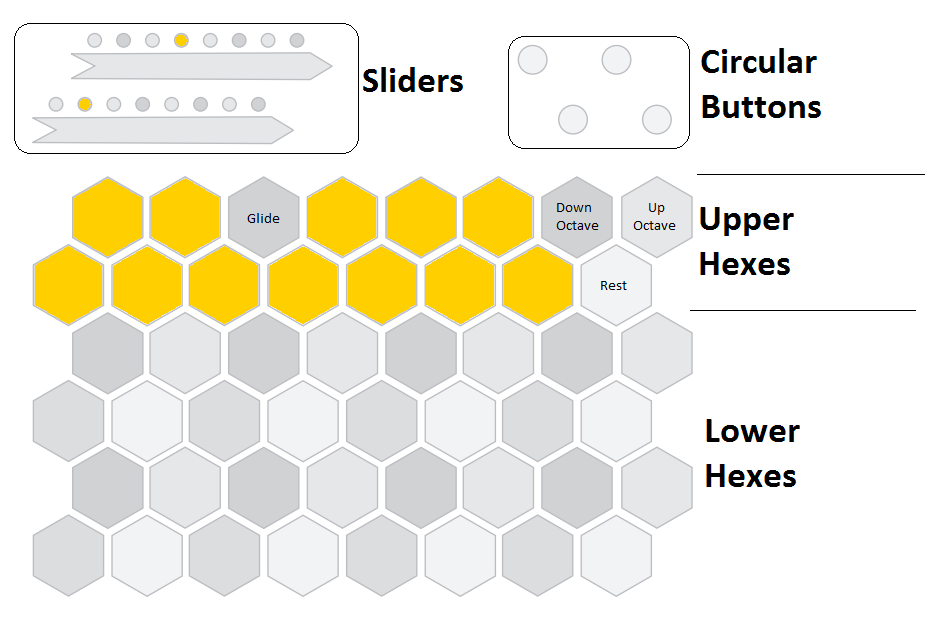
\includegraphics[width=\linewidth]{default.png}
  \end{figure}

  To further edit hexes that are already added, you can hit the top-right circular button
  and it will turn red to indicate you are in Edit Mode. You can now select hexes to edit
  their pitch and CV values, as well as the note length. If you would like to edit more
  than one hex value at once, you can multi-select in Edit Mode by holding a selected hex
  down and picking more hexes. Once you have selected a hex (or hexes, indicated by
  red LED), the list below covers all the values that can be changed for that
  hex (or hexes) and how to do so:
  \begin{itemize}
    \item 1V/O Pitch Class: Pick the note on the keybed presented
    on the upper hexes.
    \item 1V/O Octave: Press the top-right most hexes to transpose
    down or up and octave.

    \item CV1 Value: Press the top slider to change CV1 output value.
    \item CV2 Value: Press the bottom slider to change CV2 output value.
    \item CV3 Value: First, access the secondary CV values by pressing the top-left
    circular button until it is amber.
    Then, press the top slider to change CV3 output value.
    \item CV4 Value: First, access the secondary CV values by pressing the top-left
    circular button until it is amber.
    Then, press the bottom slider to change CV3 output value.

    \item Octave Value: First, access the access the misc. slider values by pressing
    the top-left circular button until it is red.
    Then, press the top slider to change to change the octave value.
    \item Note Length Value: First, access the access the misc. slider values by pressing
    the top-left circular button until it is red.
    Then, press the bottom slider to change to change the note length value.

    \item Pitch Glide Time: Press and hold the upper hex that lies between D\#
    and F\# to access the glide times. Press the upper slider to change the pitch
    glide time. Note this is the time to glide TO this note.
    \item CV Glide Time: Press and hold the upper hex that lies between D\#
    and F\# to access the glide times. Press the lower slider to change the CV
    glide time. Note this is the time to glide TO this hex CV value.
  \end{itemize}

  All the above values can be changed for each of the 32 hexes in the
  sequence. It should be noted that you actually have two sequencers running
  at once! Pressing the bottom-left circular button will turn it red and present
  you with the Menu Page. From here you can select Sequencer Mode and Order
  (covered below), but most importantly you can access the second sequencer by
  pressing the top-right most hex.

  The second sequencer (S2) acts similarly to the first (S1) but they run in parallel.

  Okay, so I've changed all these values, but now how do I get these values out of my
  \emph{MantaMate}?! First, we need to clock the \emph{MantaMate} from the ClkIn input
  (or use the internal clock, see: \ref{refInternalClock}).
  Then you can get the pitch/CV/gate from the respective outputs (where each cell
  represents a \emph{MantaMate} output):

  \begin{center}
  \begin{tabular}{ | m{1.5cm} | m{1.5cm}| m{1.5cm} | }
    \hline
    \texttt{S1: 1V/O} & \texttt{S1: Gate} & \texttt{S1: CV1} \\
    \hline
    \texttt{S1: CV2} & \texttt{S1: CV3} & \texttt{S1: CV4} \\
    \hline
    \texttt{S2: 1V/O} & \texttt{S2: Gate} & \texttt{S2: CV1} \\
    \hline
    \texttt{S2: CV2} & \texttt{S2: CV3} & \texttt{S2: CV4} \\
    \hline
  \end{tabular}
  \end{center}

  The gate out for each sequencer is the clock modified
  by the note length values of each hex, useful for triggering an ADSR or the like.


  \subsection{Left Option Menu}

  Fill in everything the left option menu does.

  Check out section 4 for possible copy-pasteable content from before the menu switch

  \subsection{Right Option Menu}

  Fill in everything the right option menu does

  \subsection{Sequencer Outputs}

  While using a \emph{Manta} host device, the \emph{MantaMate's} outputs are divided
  into to two separate sequencers. The first two rows of outputs are for the first
  sequencer, while the third and fourth rows are for sequencer two.

  The two sequencers can be changed to pitched, trigger, or even playable keyboard controller
  independently of each other.

  \subsubsection{Pitched Mode Outputs}

  Below outlines the \emph{MantaMate's} output of a sequencer when in pitched mode.
  Note, this output will correspond to row 1 and 2 if the first sequencer is in pitched
  mode, and 3 and 4 if the second sequencer is in pitched mode.


  \begin{center}
  \begin{tabular}{ | m{1.5cm} | m{1.5cm}| m{1.5cm} | }
    \hline
    \texttt{1V/O} & \texttt{Gate} & \texttt{CV1} \\
    \hline
    \texttt{CV2} & \texttt{CV3} & \texttt{CV4} \\
    \hline
  \end{tabular}
  \end{center}

  \subsubsection{Trigger Mode Outputs}
  Below outlines the \emph{MantaMate's} output of a sequencer when in trigger mode.
  Note, this output will correspond to row 1 and 2 if the first sequencer is in trigger
  mode, and 3 and 4 if the second sequencer is in trigger mode.

  \begin{center}
  \begin{tabular}{ | m{1.5cm} | m{1.5cm}| m{1.5cm} | }
    \hline
    \texttt{CV1} & \texttt{Trigger 1} & \texttt{Trigger 2} \\
    \hline
    \texttt{CV2} & \texttt{Trigger 3} & \texttt{Trigger 4} \\
    \hline
  \end{tabular}
  \end{center}


\subsection{Saving a Sequencer Pattern}

  Explain saving a sequencer pattern.

  WARNING: This only saves the sequence for your current session.
  If you would like to save a preset, see \ref{refSavingPreset}

\subsection{Saving a Preset} \label{refSavingPreset}

  Explain saving a preset.




\section{Preferences}

  In order to edit the preferences, hit the lower-right button labeled \texttt{P}.
  In order to access a subpreference, go to the corresponding preference menu
  and then hit the save button in the lower-right labeled \texttt{S}.

  While in any of the three preference menus, the lower-right LED will be lit.

  \subsection{Tuning and MIDI Learn}

  In order to enter this preference menu, hit the lower-right \texttt{P} once.

  \subsection{Glide}

  In order to enter this preference menu, hit the lower-right \texttt{P} twice.

  \subsection{Internal Clock}\label{refInternalClock}

  In order to enter this preference menu, hit the lower-right \texttt{P} three times.


\section{Monophonic Contoller Preset}

  Switching the \emph{MantaMate} to preset 01 sets it to the global
  Monophonic Controller Mode.

  The monophonic controller has an output for 1V/O, gate, as well
  as a CV that corresponds to the surface area coverage of the current
  hex.

  \begin{center}
  \begin{tabular}{ | m{1.5cm} | m{1.5cm}| m{1.5cm} | }
    \hline
    \texttt{V1: 1V/O} & \texttt{V1: Gate} & \texttt{V1: CV} \\
    \hline
    \texttt{Unused} & \texttt{Unused} & \texttt{Unused} \\
    \hline
    \texttt{Unused} & \texttt{Unused} & \texttt{Unused} \\
    \hline
    \texttt{Unused} & \texttt{Unused} & \texttt{Unused} \\
    \hline
  \end{tabular}
  \end{center}


\section{Duophonic Contoller Preset}

  Switching the \emph{MantaMate} to preset 02 sets it to the global
  Duophonic Controller Mode.

  The duophonic controller has two sets of outputs for 1V/O, gate, as well
  as a CV that corresponds to the surface area coverage of the current
  hex.

  \begin{center}
  \begin{tabular}{ | m{1.5cm} | m{1.5cm}| m{1.5cm} | }
    \hline
    \texttt{V1: 1V/O} & \texttt{V1: Gate} & \texttt{V1: CV} \\
    \hline
    \texttt{V2: 1V/O} & \texttt{V2: Gate} & \texttt{V2: CV} \\
    \hline
    \texttt{Unused} & \texttt{Unused} & \texttt{Unused} \\
    \hline
    \texttt{Unused} & \texttt{Unused} & \texttt{Unused} \\
    \hline
  \end{tabular}
  \end{center}


\section{Triophonic Contoller Preset}

  Switching the \emph{MantaMate} to preset 03 sets it to the global
  Triophonic Controller Mode.

  The triophonic controller has three sets of outputs for 1V/O, gate, as well
  as a CV that corresponds to the surface area coverage of the current
  hex.

  \begin{center}
  \begin{tabular}{ | m{1.5cm} | m{1.5cm}| m{1.5cm} | }
    \hline
    \texttt{V1: 1V/O} & \texttt{V1: Gate} & \texttt{V1: CV} \\
    \hline
    \texttt{V2: 1V/O} & \texttt{V2: Gate} & \texttt{V2: CV} \\
    \hline
    \texttt{V3: 1V/O} & \texttt{V3: Gate} & \texttt{V3: CV} \\
    \hline
    \texttt{Unused} & \texttt{Unused} & \texttt{Unused} \\
    \hline
  \end{tabular}
  \end{center}


\section{Tetraphonic Controller Preset}

  Switching the \emph{MantaMate} to preset 04 sets it to the global
  Tetraphonic Controller Mode.

  The tetraphonic controller has four sets of outputs for 1V/O, gate, as well
  as a CV that corresponds to the surface area coverage of the current
  hex.

  \begin{center}
  \begin{tabular}{ | m{1.5cm} | m{1.5cm}| m{1.5cm} | }
    \hline
    \texttt{V1: 1V/O} & \texttt{V1: Gate} & \texttt{V1: CV} \\
    \hline
    \texttt{V2: 1V/O} & \texttt{V2: Gate} & \texttt{V2: CV} \\
    \hline
    \texttt{V3: 1V/O} & \texttt{V3: Gate} & \texttt{V3: CV} \\
    \hline
    \texttt{V4: 1V/O} & \texttt{V4: Gate} & \texttt{V4: CV} \\
    \hline
  \end{tabular}
  \end{center}

\section{CV Contoller Preset}

  Switching the \emph{MantaMate} to preset 05 sets it to the global
  CV Controller Mode.

  The CV controller has twelve CV outputs corresponding to 12 hex surface
  area coverage.

  \begin{center}
  \begin{tabular}{ | m{1.5cm} | m{1.5cm}| m{1.5cm} | }
    \hline
    \texttt{CV} & \texttt{CV} & \texttt{CV} \\
    \hline
    \texttt{CV} & \texttt{CV} & \texttt{CV} \\
    \hline
    \texttt{CV} & \texttt{CV} & \texttt{CV} \\
    \hline
    \texttt{CV} & \texttt{CV} & \texttt{CV} \\
    \hline
  \end{tabular}
  \end{center}

\section{Gate Contoller Preset}

  Switching the \emph{MantaMate} to preset 06 sets it to the global
  Gate Controller Mode.

  The gate controller has twelve gate outputs corresponding to 12 hexes.

  \begin{center}
  \begin{tabular}{ | m{1.5cm} | m{1.5cm}| m{1.5cm} | }
    \hline
    \texttt{Gate} & \texttt{Gate} & \texttt{Gate} \\
    \hline
    \texttt{Gate} & \texttt{Gate} & \texttt{Gate} \\
    \hline
    \texttt{Gate} & \texttt{Gate} & \texttt{Gate} \\
    \hline
    \texttt{Gate} & \texttt{Gate} & \texttt{Gate} \\
    \hline
  \end{tabular}
  \end{center}

  \section{Trigger Contoller Preset}

    Switching the \emph{MantaMate} to preset 07 sets it to the global
    Trigger Controller Mode.

    The trigger controller has twelve trigger outputs corresponding to 12 hexes.

    \begin{center}
    \begin{tabular}{ | m{1.5cm} | m{1.5cm}| m{1.5cm} | }
      \hline
      \texttt{Trigger} & \texttt{Trigger} & \texttt{Trigger} \\
      \hline
      \texttt{Trigger} & \texttt{Trigger} & \texttt{Trigger} \\
      \hline
      \texttt{Trigger} & \texttt{Trigger} & \texttt{Trigger} \\
      \hline
      \texttt{Trigger} & \texttt{Trigger} & \texttt{Trigger} \\
      \hline
    \end{tabular}
    \end{center}

% Local Variables:
% TeX-master: "lshort2e"
% mode: latex
% mode: flyspell
% End:

%%%%%%%%%%%%%%%%%%%%%%%%%%%%%%%%%%%%%%%%%%%%%%%%%%%%%%%%%%%%%%%%%
% Contents: Other Input Devices
% $Id: typeset.tex 537 2015-07-18 09:43:10Z oetiker $
%%%%%%%%%%%%%%%%%%%%%%%%%%%%%%%%%%%%%%%%%%%%%%%%%%%%%%%%%%%%%%%%%
\renewcommand{\chaptername}{Section}
\chapter{Other Input Devices}

\begin{intro}
  This section covers using other HOST devices with the \emph{MantaMate}. We hope
  that  any input device you can think of works with the \emph{MantaMate}, but we
  cannot make any guarantees. Below outlines some of the devices we tested and ensured
  worked as one would expect!
\end{intro}

\section{Computer/DAW}
  This works right? I think Jeff mentioned it worked? It'd be killer if it did.

\section{USB-MIDI Keyboard Controller}
  This definitely works but I don't know to what extent (are we guessing knobs
  MIDI channels and then converting that to CV???? If we are, we are awesome)

\section{USB Game Controller}
  Gotta test this again too

\section{Guitar Hero Controller}
  This would be silly but fun

\section{DDR Dance Pad}
  Maybe only vaguely usable but who else can say they have DDR working on Eurorack!?


% Local Variables:
% TeX-master: "lshort2e"
% mode: latex
% mode: flyspell
% End:

%%%%%%%%%%%%%%%%%%%%%%%%%%%%%%%%%%%%%%%%%%%%%%%%%%%%%%%%%%%%%%%%%
% Contents: No Input Device
% $Id: typeset.tex 537 2015-07-18 09:43:10Z oetiker $
%%%%%%%%%%%%%%%%%%%%%%%%%%%%%%%%%%%%%%%%%%%%%%%%%%%%%%%%%%%%%%%%%
\renewcommand{\chaptername}{Section}
\chapter{No Input Device}

\begin{intro}
  This section outlines \emph{MantaMate} presets when using no HOST device.
\end{intro}

NO DEVICE ATTACHED
(all presets include a clock out trigger on output A1)

\section{Presets}

  Each of the \emph{MantaMate} presets has a clock output on the A1 output.
  The remainder of the outputs vary as follows:

  \textbf{0}
  11 Random voltages on each clock

  \textbf{1}
  11 Random Gates on each clock

  \textbf{2}
  11 Random Triggers on each clock

  \textbf{3}
  Consecutive integer dividers -- random voltages

  \textbf{4}
  Consecutive integer dividers -- gates

  \textbf{5}
  Consecutive integer dividers -- triggers

  \textbf{6}
  Consecutive integer dividers -- toggles

  \textbf{7}
  Power of 2 dividers -- random voltages

  \textbf{8}
  Power of 2 dividers -- gates

  \textbf{9}
  Power of 2 dividers -- triggers

  \textbf{10}
  Power of 2 dividers -- toggles

  \textbf{Presets 11-18 use randomly generated patterns that repeat}

  \textbf{11}
  All patterns same length -- random voltages

  \textbf{12}
  All patterns same length -- gates

  \textbf{13}
  All patterns same length -- triggers

  \textbf{14}
  All patterns same length -- toggles

  \textbf{15}
  Each pattern has its own random length -- random voltages

  \textbf{16}
  Each pattern has its own random length -- gates

  \textbf{17}
  Each pattern has its own random length -- triggers

  \textbf{18}
  Each pattern has its own random length -- toggles

  \textbf{19-99}
  User storable presets (save the randomly generated patterns)


  The No Device functionality is activated by pressing the up or down button
  while no device is plugged into the MantaMate.
  It will then continue until power is turned off or a device is plugged in.

  The repeating random patterns are generated on power-up.
  Each of the 11 available outputs has its own pattern that is 32 steps long.

  You can generate new ones by holding down the Preferences button and then
  pressing the up or down buttons.

  Pressing up results in a compeletely new random pattern.
  Pressing down subtly changes the current patterns.

  There is a Pattern Length parameter that is set by going into the first
  preference menu (tuning) and pressing S to get to the sub-menu.
  You can then alter the length parameter.
  In the case of the "all patterns same length" presets,
  this Pattern Length enforces the reset of all patterns,
  so that they all cycle at the same time.
  In the case of "each pattern has its own random length"
  presets, the Pattern Length is treated as a "maximum pattern length"
  and will reset any patterns that are not already repeating in a shorter
  time period. The value defaults to 16, and valid values are 1-32.


% Local Variables:
% TeX-master: "lshort2e"
% mode: latex
% mode: flyspell
% End:

%%%%%%%%%%%%%%%%%%%%%%%%%%%%%%%%%%%%%%%%%%%%%%%%%%%%%%%%%%%%%%%%%
% Contents: No Input Device
% $Id: typeset.tex 537 2015-07-18 09:43:10Z oetiker $
%%%%%%%%%%%%%%%%%%%%%%%%%%%%%%%%%%%%%%%%%%%%%%%%%%%%%%%%%%%%%%%%%
\renewcommand{\chaptername}{Section}
\chapter{REMOVE THIS LATER}

OLD STUFF FROM PREVIOUS ITERATIONS OF MM. DONT FORGET TO REMOVE

  In order to change the sequencer mode and order, first access the Menu Page
  by hitting the bottom-left circular button on the \emph{Manta}.

  \begin{figure}[h!]
    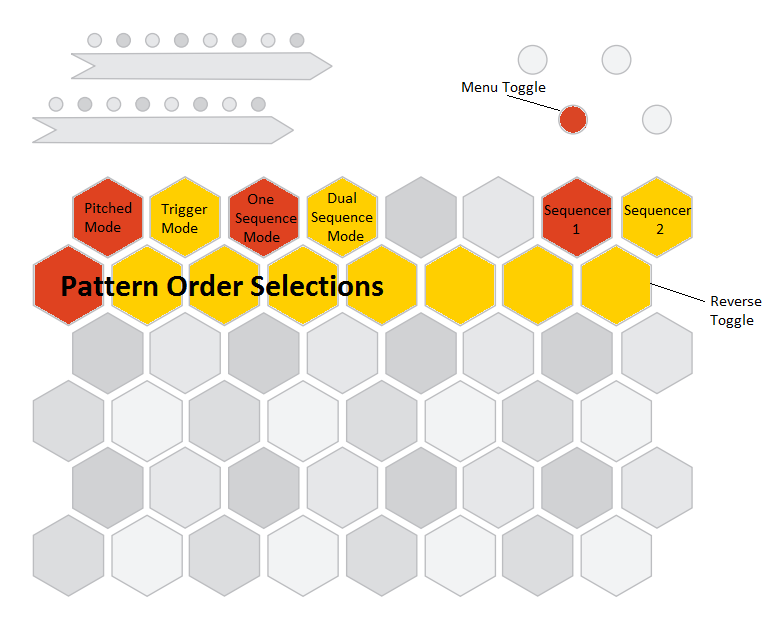
\includegraphics[width=\linewidth]{menu.png}
  \end{figure}

  There are four (TODO: Five?) sequencer modes the Manta can be in that are accessed by the
  the top-left four Hexes in the Menu Page:

  From left to right:
  \begin{itemize}
    \item Pitched (default)
    \item Dual-Sequence Pitched
    \item Trigger
    \item Dual-Sequence Trigger
    \item Mixed (TODO?)
  \end{itemize}

  Although the naming seems to imply otherwise, both Pitched Mode and
  Dual-Sequence Pitched Mode have two running sequences. The difference
  lies in that the Dual-Sequence Pitched Mode presents the user both
  sequences on the same page, while the two sequences in Pitched Mode must
  be flipped between using the two rightmost hexes in the Menu Page.

  The above is also true of Trigger Mode and Dual-Sequence Trigger Mode.

  The Menu Page also allows you to switch the sequence order mode,
  these can be changed by the second row of hexes:

  From left to right:
  \begin{itemize}
    \item Left to right, bottom to top
    \item Left to right, top to bottom
    \item Diagonally up
    \item Diagonally down
    \item Caterpillar
    \item Order in which hexes are added
    \item Random
    \item Reverse the currently selected order mode. Or turn random mode to
    a random walk pattern.
  \end{itemize}


% Local Variables:
% TeX-master: "lshort2e"
% mode: latex
% mode: flyspell
% End:

%%%%%%%%%%%%%%%%%%%%%%%%%%%%%%%%%%%%%%%%%%%%%%%%%%%%%%%%%%%%%%%%%
% Contents: Math typesetting with LaTeX
% $Id: math.tex 534 2015-04-09 13:03:16Z oetiker $
%
% Changes by Stefan M. Moser: 2008/10/22
%
% -Section 2: "Single Equations": added comment about preference of
%  equation* over \[
% -Replaced (almost) all examples with \[ by equation*
% -New section 4: "Single Equations that are Too Long: multline"
% -New section 5: "Multiple Equations"
% -Section 6: "Arrays and Matrices": made a full section and added
%  some material
% -Section 9: "Theorems, Lemmas, ...": added a subsection about proofs
%  with new material
%
% Other Changes:
% -in lshort.sty: 
%    *example environment adapted: changed in three places
%     \textwidth by \linewidth. This is necessary for
%     example-environment within a itemize-list.
%    *added \RequirePackage[retainorgcmds]{IEEEtrantools}
%
% THINGS TO DO:
% -adapt typesetting of new sections to rest of lshort, including all
%  the usual commands used so far. In particular, I guess we have to
%  get rid of the \verb-commands everywhere
% -include index-commands
%%%%%%%%%%%%%%%%%%%%%%%%%%%%%%%%%%%%%%%%%%%%%%%%%%%%%%%%%%%%%%%%%
 
\chapter{Typesetting Mathematical Formulae}

\begin{intro}
  Now you are ready! In this chapter, we will attack the main strength
  of \TeX{}: mathematical typesetting. But be warned, this chapter
  only scratches the surface. While the things explained here are
  sufficient for many people, don't despair if you can't find a
  solution to your mathematical typesetting needs here. It is highly likely
  that your problem is addressed in \AmS-\LaTeX{}.
\end{intro}
  


\section{The \texorpdfstring{\AmS}{AMS}-\LaTeX{} bundle}

If you want to typeset (advanced) \wi{mathematics}, you should
use \AmS-\LaTeX{}. The \AmS-\LaTeX{} bundle is a collection of packages and classes for
mathematical typesetting. We will mostly deal with the \pai{amsmath} package
which is a part of the bundle. \AmS-\LaTeX{} is produced by The \emph{\wi{American Mathematical Society}} 
and it is used extensively for mathematical typesetting. \LaTeX{} itself does provide
some basic features and environments for mathematics, but they are limited (or
maybe it's the other way around: \AmS-\LaTeX{} is \emph{unlimited}!) and
in some cases inconsistent. 

\AmS-\LaTeX{} is a part of the required distribution and is provided
with all recent \LaTeX{} distributions.\footnote{If yours is missing it, go to
  \CTAN|pkg/amslatex|.} In this chapter, we assume
  \pai{amsmath} is loaded in the preamble; \verb|\usepackage{amsmath}|.

\section{Single Equations}
  
A mathematical formula can be typeset in-line within a paragraph (\emph{\wi{text style}}), or the paragraph can be broken and the formula typeset separately
(\emph{\wi{display style}}). Mathematical \wi{equation}s 
\emph{within} a paragraph are entered \index{$@\texttt{\$}} %$
between \texttt{\$} and \texttt{\$}:
\begin{example}
Add $a$ squared and $b$ squared
to get $c$ squared. Or, using 
a more mathematical approach:
$a^2 + b^2 = c^2$
\end{example}
\begin{example}
\TeX{} is pronounced as 
$\tau\epsilon\chi$\\[5pt]
100~m$^{3}$ of water\\[5pt]
This comes from my $\heartsuit$
\end{example}

If you want your larger equations to be set apart
from the rest of the paragraph, it is preferable to \emph{display} them
rather than to break the paragraph apart.
To do this, you enclose them between \verb|\begin{|\ei{equation}\verb|}| and
\verb|\end{equation}|.\footnote{This is an \textsf{amsmath} command. If you don't
have access to the package for some obscure reason, you can use \LaTeX's own
\ei{displaymath} environment instead.} You can then \ci{label} an equation number and refer to
it somewhere else in the text by using the \ci{eqref} command. If you want to
name the equation something specific, you \ci{tag} it instead.
\begin{example}
Add $a$ squared and $b$ squared
to get $c$ squared. Or, using
a more mathematical approach
 \begin{equation}
   a^2 + b^2 = c^2
 \end{equation}
Einstein says
 \begin{equation}
   E = mc^2 \label{clever}
 \end{equation}
He didn't say
 \begin{equation}
  1 + 1 = 3 \tag{dumb}
 \end{equation}
This is a reference to 
\eqref{clever}. 
\end{example}

If you don't want \LaTeX{} to number the equations, use the starred
version of \texttt{equation} using an asterisk, \ei{equation*}, or even easier, enclose the
equation in \ci{[} and \ci{]}:\footnote{\index{equation!\textsf{amsmath}}
  \index{equation!\LaTeX{}}This is again from \textsf{amsmath}. Standard \LaTeX{}'s has only the \texttt{equation} environment without the star.}
\begin{example}
Add $a$ squared and $b$ squared
to get $c$ squared. Or, using
a more mathematical approach
 \begin{equation*}
   a^2 + b^2 = c^2
 \end{equation*}
or you can type less for the
same effect:
 \[ a^2 + b^2 = c^2 \]
\end{example}
While \ci{[} is short and sweet, it does not allow switching between numbered and not numbered style as easily as
\ei{equation} and \ei{equation*}.

Note the difference in typesetting style between \wi{text style} and \wi{display style}
equations: 
\begin{example}
This is text style: 
$\lim_{n \to \infty} 
 \sum_{k=1}^n \frac{1}{k^2} 
 = \frac{\pi^2}{6}$.
And this is display style:
 \begin{equation}
  \lim_{n \to \infty} 
  \sum_{k=1}^n \frac{1}{k^2} 
  = \frac{\pi^2}{6}
 \end{equation}
\end{example}

In text style, enclose tall or deep math expressions or sub
expressions in \ci{smash}. This makes \LaTeX{} ignore the height of
these expressions. This keeps the line spacing even.

\begin{example}
A $d_{e_{e_p}}$ mathematical
expression  followed by a
$h^{i^{g^h}}$ expression. As
opposed to a smashed 
\smash{$d_{e_{e_p}}$} expression 
followed by a
\smash{$h^{i^{g^h}}$} expression.
\end{example}

\subsection{Math Mode}

There are also differences between \emph{\wi{math mode}} and \emph{text mode}. For
example, in \emph{math mode}: 

\begin{enumerate}

\item \index{spacing!math mode} Most spaces and line breaks do not have any significance, as all spaces
are either derived logically from the mathematical expressions, or
have to be specified with special commands such as \ci{,}, \ci{quad} or
\ci{qquad} (we'll get back to that later, see section~\ref{sec:math-spacing}).
 
\item Empty lines are not allowed. Only one paragraph per formula.

\item Each letter is considered to be the name of a variable and will be
typeset as such. If you want to typeset normal text within a formula
(normal upright font and normal spacing) then you have to enter the
text using the \verb|\text{...}| command (see also section \ref{sec:fontsz} on
page \pageref{sec:fontsz}).

\end{enumerate}
\begin{example}
$\forall x \in \mathbf{R}:
 \qquad x^{2} \geq 0$
\end{example}
\begin{example}
$x^{2} \geq 0\qquad
 \text{for all }x\in\mathbf{R}$
\end{example}
 
Mathematicians can be very fussy about which symbols are used:
it would be conventional here to use the `\wi{blackboard bold}' font,
\index{bold symbols} which is obtained using \ci{mathbb} from the
package \pai{amssymb}.\footnote{\pai{amssymb} is not a part
  of the \AmS-\LaTeX{} bundle, but it is perhaps still a part of your \LaTeX{}
  distribution. Check your distribution
  or go to \texttt{CTAN:/fonts/amsfonts/latex/} to obtain it.}
\ifx\mathbb\undefined\else
The last example becomes
\begin{example}
$x^{2} \geq 0\qquad
 \text{for all } x 
 \in \mathbb{R}$
\end{example}
\fi
See Table~\ref{mathalpha} on page~\pageref{mathalpha} and
Table~\ref{mathfonts} on page~\pageref{mathfonts} for more math fonts.



\section{Building Blocks of a Mathematical Formula}

In this section, we describe the most important commands used in mathematical
typesetting. Most of the commands in this section will not require
\textsf{amsmath} (if they do, it will be stated clearly), but load it anyway.


\textbf{Lowercase \wi{Greek letters}} are entered as \verb|\alpha|,
 \verb|\beta|, \verb|\gamma|, \ldots, uppercase letters
are entered as \verb|\Gamma|, \verb|\Delta|, \ldots\footnote{There is no
  uppercase Alpha, Beta etc. defined in \LaTeXe{} because it looks the same as a
  normal roman A, B\ldots{}} 

Take a look at Table~\ref{greekletters} on page~\pageref{greekletters} for a
list of Greek letters.
\begin{example}
$\lambda,\xi,\pi,\theta,
 \mu,\Phi,\Omega,\Delta$
\end{example}


\textbf{Exponents, Superscripts and Subscripts} can be specified using\index{exponent}\index{subscript}\index{superscript}
the \verb|^|\index{^@\verb"|^"|} and the \verb|_|\index{_@\verb"|_"|} characters.
Most math mode commands act only on the next character, so if you
want a command to affect several characters, you have to group them
together using curly braces: \verb|{...}|.

Table~\ref{binaryrel} on page \pageref{binaryrel} lists a lot of binary
relations like $\subseteq$ and $\perp$.

\begin{example}
$p^3_{ij} \qquad 
 m_\text{Knuth}\qquad
\sum_{k=1}^3 k \\[5pt]
 a^x+y \neq a^{x+y}\qquad 
 e^{x^2} \neq {e^x}^2$
\end{example}


The \textbf{\wi{square root}} is entered as \ci{sqrt}; the
$n^\text{th}$ root is generated with \verb|\sqrt[|$n$\verb|]|. The size of
the root sign is determined automatically by \LaTeX. If just the sign
is needed, use \verb|\surd|.

See various kinds of arrows like $\hookrightarrow$ and $\rightleftharpoons$ on
Table~\ref{tab:arrows} on page \pageref{tab:arrows}. 
\begin{example}
$\sqrt{x} \Leftrightarrow x^{1/2}
 \quad \sqrt[3]{2}
 \quad \sqrt{x^{2} + \sqrt{y}}
 \quad \surd[x^2 + y^2]$
\end{example}


\index{dots!three}
\index{vertical!dots}
\index{horizontal!dots}
While the \textbf{\wi{dot}} sign to indicate
the multiplication operation is normally left out, it is sometimes written
to help the eye in grouping a formula.
Use \ci{cdot} to typeset a single centered dot. \ci{cdots} is
three centered \textbf{\wi{dots}} while \ci{ldots} sets the dots low (on the
baseline). Besides that, there are \ci{vdots} for 
vertical and \ci{ddots} for \wi{diagonal dots}. There are more examples in 
section~\ref{sec:arraymat}.
\begin{example}
$\Psi = v_1 \cdot v_2
 \cdot \ldots \qquad 
 n! = 1 \cdot 2 
 \cdots (n-1) \cdot n$
\end{example}

The commands \ci{overline} and \ci{underline} create
\textbf{horizontal lines} directly over or under an expression:
\index{horizontal!line} \index{line!horizontal}
\begin{example}
$0.\overline{3} = 
 \underline{\underline{1/3}}$
\end{example}

The commands \ci{overbrace} and \ci{underbrace} create
long \textbf{horizontal braces} over or under an expression:
\index{horizontal!brace} \index{brace!horizontal} 
\begin{example}
$\underbrace{\overbrace{a+b+c}^6 
 \cdot \overbrace{d+e+f}^7}
 _\text{meaning of life} = 42$
\end{example}

\index{mathematical!accents} To add mathematical accents such as \textbf{small
arrows} or \textbf{\wi{tilde}} signs to variables, the commands
given in Table~\ref{mathacc} on page~\pageref{mathacc} might be useful.  Wide hats and
tildes covering several characters are generated with \ci{widetilde}
and \ci{widehat}. Notice the difference between \ci{hat} and \ci{widehat} and the placement of
\ci{bar} for a variable with subscript. The \wi{apostrophe} mark
\verb|'|\index{'@\verb"|'"|} gives a \wi{prime}:
% a dash is --
\begin{example}
$f(x) = x^2 \qquad f'(x) 
 = 2x \qquad f''(x) = 2\\[5pt]
 \hat{XY} \quad \widehat{XY}
 \quad \bar{x_0} \quad \bar{x}_0$
\end{example}


\textbf{Vectors}\index{vectors} are often specified by adding small
\wi{arrow symbols} on the tops of variables. This is done with the
\ci{vec} command. The two commands \ci{overrightarrow} and
\ci{overleftarrow} are useful to denote the vector from $A$ to $B$:
\begin{example}
$\vec{a} \qquad
 \vec{AB} \qquad
 \overrightarrow{AB}$
\end{example}


Names of functions are often typeset in an upright
font, and not in italics as variables are, so \LaTeX{} supplies the
following commands to typeset the most common function names:
\index{mathematical!functions}

\begin{tabular}{llllll}
\ci{arccos} &  \ci{cos}  &  \ci{csc} &  \ci{exp} &  \ci{ker}    & \ci{limsup} \\
\ci{arcsin} &  \ci{cosh} &  \ci{deg} &  \ci{gcd} &  \ci{lg}     & \ci{ln}     \\
\ci{arctan} &  \ci{cot}  &  \ci{det} &  \ci{hom} &  \ci{lim}    & \ci{log}    \\
\ci{arg}    &  \ci{coth} &  \ci{dim} &  \ci{inf} &  \ci{liminf} & \ci{max}    \\
\ci{sinh}   & \ci{sup}   &  \ci{tan}  & \ci{tanh}&  \ci{min}    & \ci{Pr}     \\
\ci{sec}    & \ci{sin} \\
\end{tabular}

\begin{example}
\begin{equation*}
  \lim_{x \rightarrow 0}
  \frac{\sin x}{x}=1
\end{equation*}
\end{example}

For functions missing from the list, use the \ci{DeclareMathOperator}
command. There is even a starred version for functions with limits.
This command works only in the preamble so the commented lines in the
example below must be put into the preamble.

\begin{example}
%\DeclareMathOperator{\argh}{argh}
%\DeclareMathOperator*{\nut}{Nut}
\begin{equation*}
  3\argh = 2\nut_{x=1}    
\end{equation*}
\end{example}

For the \wi{modulo function}, there are two commands: \ci{bmod} for the
binary operator ``$a \bmod b$'' and \ci{pmod}
for expressions
such as ``$x\equiv a \pmod{b}$:''
\begin{example}
$a\bmod b \\
 x\equiv a \pmod{b}$
\end{example}

A built-up \textbf{\wi{fraction}} is typeset with the
\ci{frac}\verb|{...}{...}| command. In in-line equations, the fraction is shrunk to
fit the line. This style is obtainable in display style with \ci{tfrac}. The
reverse, i.e.\ display style fraction in text, is made with \ci{dfrac}.
Often the slashed form $1/2$ is preferable, because it looks better
for small amounts of `fraction material:'
\begin{example}
In display style:
\begin{equation*}
  3/8 \qquad \frac{3}{8} 
  \qquad \tfrac{3}{8}
\end{equation*}
\end{example}

\begin{example}
In text style:
$1\frac{1}{2}$~hours \qquad
$1\dfrac{1}{2}$~hours
\end{example}
 
Here the \ci{partial} command for \wi{partial derivative}s is used:
\begin{example}
\begin{equation*} 
  \sqrt{\frac{x^2}{k+1}}\qquad
  x^\frac{2}{k+1}\qquad
  \frac{\partial^2f}
  {\partial x^2} 
\end{equation*}
\end{example}

To typeset \wi{binomial coefficient}s or similar structures, use
the command \ci{binom} from \pai{amsmath}:
\begin{example}
Pascal's rule is
\begin{equation*}
 \binom{n}{k} =\binom{n-1}{k}
 + \binom{n-1}{k-1}
\end{equation*}
\end{example}

For \wi{binary relations} it may be useful to stack symbols over each other.
\ci{stackrel}\verb|{#1}{#2}| puts the symbol given
in \verb|#1| in superscript-like size over \verb|#2| which
is set in its usual position.
\begin{example}
\begin{equation*}
 f_n(x) \stackrel{*}{\approx} 1
\end{equation*}
\end{example}

The \textbf{\wi{integral operator}} is generated with \ci{int}, the
\textbf{\wi{sum operator}} with \ci{sum}, and the \textbf{\wi{product operator}}
with \ci{prod}. The upper and lower limits are specified with~\verb|^|
and~\verb|_| like subscripts and superscripts:
\begin{example}
\begin{equation*}
\sum_{i=1}^n \qquad
\int_0^{\frac{\pi}{2}} \qquad
\prod_\epsilon
\end{equation*}
\end{example}

To get more control over the placement of indices in complex
expressions, \pai{amsmath} provides the \ci{substack} command:
\begin{example}
\begin{equation*}
\sum^n_{\substack{0<i<n \\ 
        j\subseteq i}}
   P(i,j) = Q(i,j)
\end{equation*}
\end{example}



\LaTeX{} provides all sorts of symbols for \textbf{\wi{bracketing}} and other
\textbf{\wi{delimiters}} (e.g.~$[\;\langle\;\|\;\updownarrow$).
Round and square brackets can be entered with the corresponding keys and
curly braces with \verb|\{|, but all other delimiters are generated with
special commands (e.g.~\verb|\updownarrow|).
\begin{example}
\begin{equation*}
{a,b,c} \neq \{a,b,c\}
\end{equation*}
\end{example}

If you put \ci{left} in front of an opening delimiter and
\ci{right} in front of a closing delimiter, \LaTeX{} will automatically
determine the correct size of the delimiter. Note that you must close
every \ci{left} with a corresponding \ci{right}. If you
don't want anything on the right, use the invisible ``\ci{right.}'':
\begin{example}
\begin{equation*}
1 + \left(\frac{1}{1-x^{2}}
    \right)^3 \qquad 
\left. \ddagger \frac{~}{~}\right)
\end{equation*}
\end{example}

In some cases it is necessary to specify the correct size of a
mathematical delimiter\index{mathematical!delimiter} by hand,
which can be done using the commands \ci{big}, \ci{Big}, \ci{bigg} and
\ci{Bigg} as prefixes to most delimiter commands:
\begin{example}
$\Big((x+1)(x-1)\Big)^{2}$\\
$\big( \Big( \bigg( \Bigg( \quad
\big\} \Big\} \bigg\} \Bigg\} \quad
\big\| \Big\| \bigg\| \Bigg\| \quad
\big\Downarrow \Big\Downarrow 
\bigg\Downarrow \Bigg\Downarrow$
\end{example}
 For a list of all delimiters available, see Table~\ref{tab:delimiters} on page
\pageref{tab:delimiters}. 


\section{Single Equations that are Too Long: multline}
\index{long equations}
\label{sec:multline}

If an equation is too long, we have to wrap it somehow. Unfortunately,
wrapped equations are usually less easy to read than not wrapped
ones. To improve the readability, there are certain rules on how to do
the wrapping:
\begin{enumerate}
\item In general one should always wrap an equation \textbf{before} an
  equality sign or an operator.
\item A wrap before an equality sign is preferable to a wrap before
  any operator.
\item A wrap before a plus- or minus-operator is preferable to a wrap
  before a multiplication-operator.
\item Any other type of wrap should be avoided if at all possible.
\end{enumerate}
The easiest way to achieve such a wrapping is the use of the
\ei{multline} en\-vi\-ron\-ment:\footnote{The
  \texttt{multline}-environment is from \texttt{amsmath}.}
\begin{example}
\begin{multline}
  a + b + c + d + e + f 
  + g + h + i  
  \\
  = j + k + l + m + n 
\end{multline}
\end{example}
\noindent
The difference from the \ei{equation} environment is that an arbitrary
line-break (or also multiple line-breaks) can be introduced. This is
done by putting a \verb+\\+ on those places where the equation needs
to be wrapped. Similarly to \ei{equation*} there also exists a
\ei{multline*} version for preventing an equation number.

Often the
\ei{IEEEeqnarray} environment (see section~\ref{sec:IEEEeqnarray})
will yield better results.  Consider the following
situation:
\begin{example}
\begin{equation}
  a = b + c + d + e + f 
  + g + h + i + j 
  + k + l + m + n + o + p  
  \label{eq:equation_too_long}
\end{equation}
\end{example}
\noindent
Here it is actually the RHS that is too long to fit on one line. The
\ei{multline} environment creates the following output:
\begin{example}
\begin{multline}
  a = b + c + d + e + f 
  + g + h + i + j \\
  + k + l + m + n + o + p
\end{multline}
\end{example}

This is better than \eqref{eq:equation_too_long}, but
it has the disadvantage that the equality sign loses its natural
greater importance with respect to the plus operator in front of
$k$. The better solution is provided by the
\ei{IEEEeqnarray} environment that will be discussed in detail in
Section~\ref{sec:IEEEeqnarray}.

\section{Multiple Equations}
\index{equation!multiple}
\label{sec:IEEEeqnarray}

In the most general situation we have a sequence of several
equalities that do not fit onto one line. Here we need to work with
vertical alignment in order to keep the array of equations in a nice
and readable structure.

Before we offer our suggestions on how to do this, we start with a few
bad examples that show the biggest drawbacks of some common solutions.


\subsection{Problems with Traditional Commands}
\label{sec:problems_traditional}

To group multiple equations the
\ei{align} environment\footnote{The \texttt{align}-environment can
  also be used to group several blocks of equations beside each other.
  Another excellent use case for the
  \ei{IEEEeqnarray} environment. Try an argument like
  \texttt{\{rCl+rCl\}}.} could be used:
\begin{example}
\begin{align}
  a & = b + c \\
  & = d + e
\end{align}
\end{example}

this approach fails once a single line is too long:
\begin{example}
\begin{align}
  a & = b + c \\
  & = d + e + f + g + h + i 
  + j + k + l \nonumber \\
  & + m + n + o \\
  & = p + q + r + s
\end{align}
\end{example}
\noindent
Here $+\:m$ should be below $d$ and not below the equality sign. Of
course, one could add some space (\verb+\hspace{...}+),
but this will never yield a precise arrangement (and is bad
style\ldots).

A better solution is offered by the \ei{eqnarray} environment:
\begin{example}
\begin{eqnarray}
  a & = & b + c \\
  & = & d + e + f + g + h + i 
  + j + k + l \nonumber \\
  && +\: m + n + o \\
  & = & p + q + r + s
\end{eqnarray}
\end{example}

This is still not optimal. The spaces around the equality signs are too big.
Particularly, they are \textbf{not} the same as in the
\ei{multline} and \ei{equation} environments:
\begin{example}
\begin{eqnarray}
  a & = & a = a
\end{eqnarray}
\end{example}

\noindent \ldots and the expression sometimes overlaps with the equation number even
  though there would be enough room on the left:
\begin{example}
\begin{eqnarray}
  a & = & b + c 
  \\
  & = & d + e + f + g + h^2 
  + i^2 + j 
  \label{eq:faultyeqnarray}
\end{eqnarray}
\end{example}

\noindent While the environment offers a command \ci{lefteqn} that can
  be used when the LHS is too long:
\begin{example}
\begin{eqnarray}
  \lefteqn{a + b + c + d 
    + e + f + g + h}\nonumber\\
  & = & i + j + k + l + m 
  \\
  & = & n + o + p + q + r + s
\end{eqnarray}
\end{example}
\noindent This is not optimal either as the RHS is too short and the array is
not properly centered:
\begin{example}
\begin{eqnarray}
  \lefteqn{a + b + c + d 
    + e + f + g + h} 
  \nonumber \\
  & = & i + j 
\end{eqnarray}
\end{example}

\noindent Having badmouthed the competition sufficiently, I can now steer you gently towards the glorious \ldots

\subsection{IEEEeqnarray Environment}
\label{sec:IEEEeqnarray_intro}

The \ei{IEEEeqnarray} environment is a very powerful command with
many options. Here, we will only introduce its basic
functionalities. For more information please refer to the
manual.\footnote{The official manual is called
  \CTAN|macros/latex/contrib/IEEEtran/IEEEtran_HOWTO.pdf|. The part about \texttt{IEEEeqnarray}
  can be found in Appendix~F.}

First of all, in order to be able to use the
\ei{IEEEeqnarray} environment one needs to load the
package\footnote{The \pai{IEEEtrantools} package may not be included in your setup, it can be found on CTAN.}
\pai{IEEEtrantools}. Include the following line in the header of
your document: \small
\begin{verbatim}
\usepackage[retainorgcmds]{IEEEtrantools}
\end{verbatim}
\normalsize

The strength of \ei{IEEEeqnarray} is the ability to specify
the number of \emph{columns} in the equation array. Usually, this
specification will be \verb+{rCl}+, \emph{i.e.}, three columns, the
first column right-justified, the middle one centered with a little
more space around it (therefore we specify capital \texttt{C} instead of
lower-case \texttt{c}) and the third column left-justified:
\begin{example}
\begin{IEEEeqnarray}{rCl}
  a & = & b + c 
  \\
  & = & d + e + f + g + h 
  + i + j + k \nonumber\\
  && \negmedspace {} + l + m + n + o 
  \\
  & = & p + q + r + s
\end{IEEEeqnarray}
\end{example}
Any number of columns can be specified:
\verb+{c}+ will give only one column with all entries centered, or
\verb+{rCll}+ would add a fourth, left-justified column to use
for comments. Moreover, beside \texttt{l}, \texttt{c}, \texttt{r}, \texttt{L},
\texttt{C}, \texttt{R} for math mode entries there are also \texttt{s},
\texttt{t}, \texttt{u} for left, centered, and right text mode entries.
Additional space can be added with \texttt{.} and
\texttt{/} and \texttt{?} in increasing order.\footnote{For more spacing
  types refer to Section~\ref{sec:putting-qed-right}.}
Note the spaces around the equality signs in contrast to the space produced
by the \texttt{eqnarray} environment.

\subsection{Common Usage}
\label{sec:common-usage}

In the following we will describe how we use \texttt{IEEEeqnarray} to
solve the most common problems.

If a line overlaps with the equation number as in
  \eqref{eq:faultyeqnarray}, the command 
\small
\begin{verbatim}
\IEEEeqnarraynumspace
\end{verbatim} 
\normalsize
  can be used: it has to be added in the corresponding line and makes
  sure that the whole equation array is shifted by the size of the
  equation numbers (the shift depends on the size of the number!):
  instead of
\begin{example}
\begin{IEEEeqnarray}{rCl}
  a & = & b + c 
  \\
  & = & d + e + f + g + h 
  + i + j + k 
  \\
  & = & l + m + n
\end{IEEEeqnarray}
\end{example}
  we get
\begin{example}
\begin{IEEEeqnarray}{rCl}
  a & = & b + c 
  \\
  & = & d + e + f + g + h 
  + i + j + k 
  \IEEEeqnarraynumspace\\
  & = & l + m + n.
\end{IEEEeqnarray}
\end{example}

If the LHS is too long, as a replacement for the faulty
  \ci{lefteqn} command, \texttt{IEEEeqnarray} offers the
  \ci{IEEEeqnarraymulticol} command which works in all situations:
\begin{example}
\begin{IEEEeqnarray}{rCl}
  \IEEEeqnarraymulticol{3}{l}{
    a + b + c + d + e + f 
    + g + h
  }\nonumber\\ \quad
  & = & i + j 
  \\
  & = & k + l + m
\end{IEEEeqnarray}
\end{example}
The usage is identical to the \ci{multicolumns} command in the
\texttt{tabular}-en\-vi\-ron\-ment. The first argument \verb+{3}+
specifies that three columns shall be combined into one which will be
left-justified \verb+{l}+.

Note that by inserting \ci{quad} commands one can easily adapt
the depth of the equation signs,\footnote{I think that one quad is the
  distance that looks good for most cases.} \emph{e.g.},
\begin{example}
\begin{IEEEeqnarray}{rCl}
  \IEEEeqnarraymulticol{3}{l}{
    a + b + c + d + e + f 
    + g + h
  }\nonumber\\ \qquad\qquad
  & = & i + j
  \\
  & = & k + l + m
\end{IEEEeqnarray}
\end{example}

If an equation is split into two or more lines, \LaTeX\
  interprets the first $+$ or $-$ as a sign instead of operator.
  Therefore, it is necessary to add an additional space \ci{:}
  between the operator and the term: instead of
\begin{example}
\begin{IEEEeqnarray}{rCl}
  a & = & b + c 
  \\
  & = & d + e + f + g + h 
  + i + j + k \nonumber\\
  && + l + m + n + o 
  \\
  & = & p + q + r + s
\end{IEEEeqnarray}
\end{example}
  we should write
\begin{example}
\begin{IEEEeqnarray}{rCl}
  a & = & b + c 
  \\
  & = & d + e + f + g + h 
  + i + j + k \nonumber\\
  && \negmedspace {} + l + m + n + o 
  \\
  & = & p + q + r + s
\end{IEEEeqnarray}
\end{example}
\noindent Note the space difference between $+$ and $l$!
The construction \verb|{} + l| forces the \verb|+|-sign to be a binary operator rather
than just a sign, and the unwanted ensuing space between
\verb|{}| and \verb|+| is compensated by a negative medium space
\ci{negmedspace}.

If a particular line should not have an equation number, the
  number can be suppressed using \ci{nonumber} (or
  \ci{IEEEnonumber}). If on such a line a label
  \verb+\label{eq:...}+ is defined, then this label is passed on
  to the next equation number that is not suppressed. Place the labels right before the line-break
  \verb+\\+ or the next to the equation it belongs to. Apart from
  improving the readability of the source code this prevents a
  compilation error when a \ci{IEEEmulticol} command
  follows the label-definition.
  
There also exists a *-version where all equation numbers are
  suppressed. In this case an equation number can be made to appear
  using the command \ci{IEEEyesnumber}:
\begin{example}
\begin{IEEEeqnarray*}{rCl}
  a & = & b + c \\
  & = & d + e \IEEEyesnumber\\
  & = & f + g
\end{IEEEeqnarray*}
\end{example}

Sub-numbers are also easily possible using 
  \ci{IEEEyessubnumber}:
\begin{example}
\begin{IEEEeqnarray}{rCl}
  a & = & b + c 
  \IEEEyessubnumber\\
  & = & d + e 
  \nonumber\\
  & = & f + g 
  \IEEEyessubnumber  
\end{IEEEeqnarray}
\end{example}
  
\section{Arrays and Matrices} \label{sec:arraymat}

To typeset \textbf{arrays}, use the \ei{array} environment. It works
in a similar way to the \texttt{tabular} environment. The \verb|\\| command is
used to break the lines:
\begin{example}
  \begin{equation*}
    \mathbf{X} = \left( 
      \begin{array}{ccc}
        x_1 & x_2 & \ldots \\
        x_3 & x_4 & \ldots \\
        \vdots & \vdots & \ddots
      \end{array} \right)
  \end{equation*}
\end{example}

The \ei{array} environment can also be used to typeset \wi{piecewise function}s by
using a ``\verb|.|'' as an invisible \ci{right} delimiter:
\begin{example}
\begin{equation*}
  |x| = \left\{
    \begin{array}{rl}
      -x & \text{if } x < 0,\\
      0 & \text{if } x = 0,\\
      x & \text{if } x > 0.
    \end{array} \right.
\end{equation*}
\end{example}
The \ei{cases} environment from \textsf{amsmath} simplifies
the syntax, so it is worth a look:
\begin{example}
  \begin{equation*}
    |x| = 
    \begin{cases}
      -x & \text{if } x < 0,\\
      0 & \text{if } x = 0,\\
      x & \text{if } x > 0.
    \end{cases} 
\end{equation*}
\end{example}


Matrices\index{matrix} can be typeset by \ei{array}, but
\pai{amsmath} provides a better solution using the different \ei{matrix}
environments. There are six versions with different delimiters: \ei{matrix}
(none), \ei{pmatrix} $($, \ei{bmatrix} $[$, \ei{Bmatrix} $\{$, \ei{vmatrix} $\vert$ and
\ei{Vmatrix} $\Vert$. You don't have to specify the number of columns as with
\ei{array}. The maximum number is 10, but it is customisable (though it is not
very often you need 10 columns!):
\begin{example}
\begin{equation*}
  \begin{matrix} 
    1 & 2 \\
    3 & 4 
  \end{matrix} \qquad
  \begin{bmatrix} 
    p_{11} & p_{12} & \ldots 
    & p_{1n} \\
    p_{21} & p_{22} & \ldots 
    & p_{2n} \\
    \vdots & \vdots & \ddots 
    & \vdots \\
    p_{m1} & p_{m2} & \ldots 
    & p_{mn} 
  \end{bmatrix}
\end{equation*}
\end{example}



\section{Spacing in Math Mode} \label{sec:math-spacing}

\index{math spacing} If the spacing within formulae chosen by \LaTeX{}
is not satisfactory, it can be adjusted by inserting special spacing
commands: \ci{,} for $\frac{3}{18}\:\textrm{quad}$
(\demowidth{0.166em}), \ci{:} for $\frac{4}{18}\: \textrm{quad}$
(\demowidth{0.222em}) and \ci{;} for $\frac{5}{18}\: \textrm{quad}$
(\demowidth{0.277em}).  The escaped space character \verb*|\ |
generates a medium sized space comparable to the interword spacing and
\ci{quad} (\demowidth{1em}) and \ci{qquad} (\demowidth{2em}) produce
large spaces. The size of a \ci{quad} corresponds to the width of the
character `M' of the current font. \verb|\!|\cih{"!} produces a
negative space of $-\frac{3}{18}\:\textrm{quad}$
($-$\demowidth{0.166em}).

\begin{example}
\begin{equation*}
  \int_1^2 \ln x \mathrm{d}x 
  \qquad
  \int_1^2 \ln x \,\mathrm{d}x
\end{equation*}
\end{example}

Note that `d' in the differential is conventionally set in roman.
In the next example, we define a new command \ci{ud} (upright d) which produces
``$\,\mathrm{d}$'' (notice the spacing \demowidth{0.166em} before the
$\text{d}$), so we don't have to write it every time. The \ci{newcommand} is
placed in the preamble. %  More on
% \ci{newcommand} in section~\ref{} on page \pageref{}. To Do: Add label and
% reference to "Customising LaTeX" -> "New Commands, Environments and Packages"
% -> "New Commands".
\begin{example}
\newcommand{\ud}{\,\mathrm{d}}

\begin{equation*}
 \int_a^b f(x)\ud x 
\end{equation*}
\end{example}

If you want to typeset multiple integrals, you'll discover that the spacing
between the integrals is too wide. You can correct it using \ci{!}, but
\pai{amsmath} provides an easier way for fine-tuning
the spacing, namely the \ci{iint}, \ci{iiint}, \ci{iiiint}, and \ci{idotsint}
commands.

\begin{example}
\newcommand{\ud}{\,\mathrm{d}}

\begin{IEEEeqnarray*}{c}
  \int\int f(x)g(y) 
                  \ud x \ud y \\
  \int\!\!\!\int 
         f(x)g(y) \ud x \ud y \\
  \iint f(x)g(y)  \ud x \ud y 
\end{IEEEeqnarray*}
\end{example}

See the electronic document \texttt{testmath.tex} (distributed with
\AmS-\LaTeX) or Chapter 8 of \companion{} for further details.

\subsection{Phantoms}

When vertically aligning text using \verb|^| and \verb|_| \LaTeX{} is sometimes
just a little too helpful. Using the \ci{phantom} command you can
reserve space for characters that do not show up in the final output.
The easiest way to understand this is to look at an example:
\begin{example}
\begin{equation*}
{}^{14}_{6}\text{C}
\qquad \text{versus} \qquad
{}^{14}_{\phantom{1}6}\text{C}
\end{equation*}
\end{example}
If you want to typeset a lot of isotopes as in the example, the \pai{mhchem}
package is very useful for typesetting isotopes and chemical formulae too.


\section{Fiddling with the Math Fonts}\label{sec:fontsz}
Different math fonts are listed on Table~\ref{mathalpha} on page
\pageref{mathalpha}.
\begin{example}
 $\Re \qquad
  \mathcal{R} \qquad
  \mathfrak{R} \qquad
  \mathbb{R} \qquad $  
\end{example}
The last two require \pai{amssymb} or \pai{amsfonts}.

Sometimes you need to tell \LaTeX{} the correct font
size. In math mode, this is set with the following four commands:
\begin{flushleft}
\ci{displaystyle}~($\displaystyle 123$),
 \ci{textstyle}~($\textstyle 123$), 
\ci{scriptstyle}~($\scriptstyle 123$) and
\ci{scriptscriptstyle}~($\scriptscriptstyle 123$).
\end{flushleft}

If $\sum$ is placed in a fraction, it'll be typeset in text style unless you tell
\LaTeX{} otherwise:
\begin{example}
\begin{equation*}
 P = \frac{\displaystyle{ 
   \sum_{i=1}^n (x_i- x)
   (y_i- y)}} 
   {\displaystyle{\left[
   \sum_{i=1}^n(x_i-x)^2
   \sum_{i=1}^n(y_i- y)^2
   \right]^{1/2}}}
\end{equation*}    
\end{example}
Changing styles generally affects the way big operators and limits are displayed.

% This is not a math accent, and no maths book would be set this way.
% mathop gets the spacing right.


\subsection{Bold Symbols}
\index{bold symbols}

It is quite difficult to get bold symbols in \LaTeX{}; this is
probably intentional as amateur typesetters tend to overuse them.  The
font change command \verb|\mathbf| gives bold letters, but these are
roman (upright) whereas mathematical symbols are normally italic, and
furthermore it doesn't work on lower case Greek letters.
There is a \ci{boldmath} command, but \emph{this can only be used
outside math mode}. It works for symbols too, though:
\begin{example}
$\mu, M \qquad 
\mathbf{\mu}, \mathbf{M}$
\qquad \boldmath{$\mu, M$}
\end{example}

The package \pai{amsbsy} (included by \pai{amsmath}) as well as the
package \pai{bm} from the \texttt{tools} bundle make this much easier as they include
a \ci{boldsymbol} command:

\begin{example}
$\mu, M \qquad
\boldsymbol{\mu}, \boldsymbol{M}$
\end{example}


\section{Theorems, Lemmas, \ldots}

When writing mathematical documents, you probably need a way to
typeset ``Lemmas'', ``Definitions'', ``Axioms'' and similar
structures.
\begin{lscommand}
\ci{newtheorem}\verb|{|\emph{name}\verb|}[|\emph{counter}\verb|]{|%
         \emph{text}\verb|}[|\emph{section}\verb|]|
\end{lscommand}
The \emph{name} argument is a short keyword used to identify the
``theorem''. With the \emph{text} argument you define the actual name
of the ``theorem'', which will be printed in the final document.

The arguments in square brackets are optional. They are both used to
specify the numbering used on the ``theorem''. Use  the \emph{counter}
argument to specify the \emph{name} of a previously declared
``theorem''. The new ``theorem'' will then be numbered in the same
sequence.  The \emph{section} argument allows you to specify the
sectional unit within which the ``theorem'' should get its numbers.

After executing the \ci{newtheorem} command in the preamble of your
document, you can use the following command within the document.
\begin{code}
\verb|\begin{|\emph{name}\verb|}[|\emph{text}\verb|]|\\
This is my interesting theorem\\
\verb|\end{|\emph{name}\verb|}|     
\end{code}

The \pai{amsthm} package (part of \AmS-\LaTeX) provides the 
\ci{theoremstyle}\verb|{|\emph{style}\verb|}|
command which lets you define what the theorem is all about by picking
from three predefined styles: \texttt{definition} (fat title, roman body),
\texttt{plain} (fat title, italic body) or \texttt{remark} (italic
title, roman body).

This should be enough theory. The following examples should
remove any remaining doubt, and make it clear that the
\verb|\newtheorem| environment is way too complex to understand.

% actually define things
\theoremstyle{definition} \newtheorem{law}{Law}
\theoremstyle{plain}      \newtheorem{jury}[law]{Jury}
\theoremstyle{remark}     \newtheorem*{marg}{Margaret}

First define the theorems:

\begin{verbatim}
\theoremstyle{definition} \newtheorem{law}{Law}
\theoremstyle{plain}      \newtheorem{jury}[law]{Jury}
\theoremstyle{remark}     \newtheorem*{marg}{Margaret}
\end{verbatim}

\begin{example}
\begin{law} \label{law:box}
Don't hide in the witness box
\end{law}
\begin{jury}[The Twelve]
It could be you! So beware and
see law~\ref{law:box}.\end{jury}
\begin{jury}
You will disregard the last
statement.\end{jury}
\begin{marg}No, No, No\end{marg}
\begin{marg}Denis!\end{marg}
\end{example}

The ``Jury'' theorem uses the same counter as the ``Law''
theorem, so it gets a number that is in sequence with
the other ``Laws''. The argument in square brackets is used to specify 
a title or something similar for the theorem.
\begin{example}
\newtheorem{mur}{Murphy}[section]

\begin{mur} If there are two or 
more ways to do something, and 
one of those ways can result in
a catastrophe, then someone 
will do it.\end{mur}
\end{example}

The ``Murphy'' theorem gets a number that is linked to the number of
the current section. You could also use another unit, for example chapter or
subsection.

If you want to customize your theorems down to the last dot, the
\pai{ntheorem} package offers a plethora of options.


\subsection{Proofs and End-of-Proof Symbol}
\label{sec:putting-qed-right}

The \pai{amsthm} package also provides the \ei{proof} environment.

\begin{example}
\begin{proof}
 Trivial, use
 \begin{equation*}
   E=mc^2.
 \end{equation*}
\end{proof}
\end{example}

With the command \ci{qedhere} you can move the `end of proof' symbol
around for situations where it would end up alone on a line.

\begin{example}
\begin{proof}
 Trivial, use
 \begin{equation*}
   E=mc^2. \qedhere
 \end{equation*}
\end{proof}
\end{example}

Unfortunately, this correction does not work for \texttt{IEEEeqnarray}:
\begin{example}
\begin{proof}
  This is a proof that ends
  with an equation array:
  \begin{IEEEeqnarray*}{rCl}
    a & = & b + c \\
    & = & d + e. \qedhere
  \end{IEEEeqnarray*}  
\end{proof}
\end{example}
\noindent
The reason for this is the internal structure of \texttt{IEEEeqnarray}:
it always puts two invisible columns at both sides of the array that
only contain a stretchable space. By this \texttt{IEEEeqnarray} ensures
that the equation array is horizontally centered. The
\ci{qedhere} command should actually be put \emph{outside} this
stretchable space, but this does not happen as these columns are
invisible to the user.

There is a very simple remedy. Define the stretching
explicitly!
\begin{example}
\begin{proof}
  This is a proof that ends
  with an equation array:
  \begin{IEEEeqnarray*}{+rCl+x*}
    a & = & b + c \\
    & = & d + e. & \qedhere
  \end{IEEEeqnarray*}  
\end{proof}
\end{example}
\noindent
Note that the \verb=+= in \verb={+rCl+x*}= denotes stretchable spaces, one
on the left of the equations (which, if not specified, will be done
automatically by \texttt{IEEEeqnarray}!) and one on the right of the
equations. But now on the right, \emph{after} the stretching column,
we add an empty column \verb=x=. This column will only be needed on
the last line if the \ci{qedhere} command is put
there. Finally, we specify a \verb=*=. This is a null-space that
prevents \texttt{IEEEeqnarray} from adding another unwanted \verb=+=-space!

In the case of equation numbering, there is a similar problem. Comparing
\begin{example}
\begin{proof}
  This is a proof that ends
  with a numbered equation:
  \begin{equation}
    a = b + c.
  \end{equation}
\end{proof}
\end{example}
\noindent
with
\begin{example}
\begin{proof}
  This is a proof that ends
  with a numbered equation:
  \begin{equation}
    a = b + c. \qedhere
  \end{equation}
\end{proof}
\end{example}
\noindent
you notice that in the (correct) second version the $\Box$ is much
closer to the equation than in the first version.

Similarly, the correct way of putting the QED-symbol at the end of an
equation array is as follows:
\begin{example}
\begin{proof}
  This is a proof that ends
  with an equation array:
  \begin{IEEEeqnarray}{+rCl+x*}
    a & = & b + c \\
    & = & d + e. \\
    &&& \qedhere\nonumber
  \end{IEEEeqnarray}  
\end{proof}
\end{example}
\noindent
which contrasts with
\begin{example}
\begin{proof}
  This is a proof that ends
  with an equation array:
  \begin{IEEEeqnarray}{rCl}
    a & = & b + c \\
    & = & d + e.
  \end{IEEEeqnarray}  
\end{proof}
\end{example}


%

% Local Variables:
% TeX-master: "lshort"
% mode: latex
% mode: flyspell
% End:

%%%%%%%%%%%%%%%%%%%%%%%%%%%%%%%%%%%%%%%%%%%%%%%%%%%%%%%%%%%%%%%%%%
% Contents: TeX and LaTeX and AMS symbols for Maths
% $Id: lssym.tex 477 2011-06-18 13:47:14Z oetiker $
%%%%%%%%%%%%%%%%%%%%%%%%%%%%%%%%%%%%%%%%%%%%%%%%%%%%%%%%%%%%%%%%%


\section{List of Mathematical Symbols}  \label{symbols}
 
The following tables demonstrate all the symbols normally accessible
from \emph{math mode}.  

%
% Conditional Text in case the AMS Fonts are installed
%
Note that some tables show symbols only accessible after loading the \pai{amssymb}
package in the preamble of your document\footnote{The tables were derived
  from \texttt{symbols.tex} by David~Carlisle and subsequently changed
extensively as suggested by Josef~Tkadlec.}. If the \AmS{} package and
fonts are not installed on your system, have a look at
\CTANref|CTAN:pkg/amslatex|. An even more comprehensive list of
symbols can be found at \CTANref|CTAN:info/symbols/comprehensive|.
 
\begin{table}[!h]
\caption{Math Mode Accents.}  \label{mathacc}
\begin{symbols}{*3{cl}}
\W{\hat}{a}   & \W{\check}{a} & \W{\tilde}{a}       \\
\W{\grave}{a} & \W{\dot}{a}   & \W{\ddot}{a}        \\
\W{\bar}{a}   & \W{\vec}{a}   & \W{\widehat}{AAA}   \\  
\W{\acute}{a} & \W{\breve}{a} & \W{\widetilde}{AAA} \\
\W{\mathring}{a}
\end{symbols}
\end{table}
 

\begin{table}[!h]
\caption{Greek Letters.} \label{greekletters}
\bigskip
There is no uppercase of some of the letters like \ci{Alpha}, \ci{Beta} and so
on, because they look the same as normal roman letters: A, B\ldots
\begin{symbols}{*4{cl}}
 \X{\alpha}     & \X{\theta}     & \X{o}          & \X{\upsilon}  \\
 \X{\beta}      & \X{\vartheta}  & \X{\pi}        & \X{\phi}      \\
 \X{\gamma}     & \X{\iota}      & \X{\varpi}     & \X{\varphi}   \\
 \X{\delta}     & \X{\kappa}     & \X{\rho}       & \X{\chi}      \\
 \X{\epsilon}   & \X{\lambda}    & \X{\varrho}    & \X{\psi}      \\
 \X{\varepsilon}& \X{\mu}        & \X{\sigma}     & \X{\omega}    \\
 \X{\zeta}      & \X{\nu}        & \X{\varsigma}  &               \\
 \X{\eta}       & \X{\xi}        & \X{\tau} & \\
 \X{\Gamma}     & \X{\Lambda}    & \X{\Sigma}     & \X{\Psi}      \\
 \X{\Delta}     & \X{\Xi}        & \X{\Upsilon}   & \X{\Omega}    \\
 \X{\Theta}     & \X{\Pi}        & \X{\Phi} 
\end{symbols}
\end{table}



\begin{table}[!tbp]
\caption{Binary Relations.} \label{binaryrel}
\bigskip
You can negate the following symbols by prefixing them with a \ci{not} command.
\begin{symbols}{*3{cl}}
 \X{<}           & \X{>}           & \X{=}          \\
 \X{\leq}or \verb|\le|   & \X{\geq}or \verb|\ge|   & \X{\equiv}     \\
 \X{\ll}         & \X{\gg}         & \X{\doteq}     \\
 \X{\prec}       & \X{\succ}       & \X{\sim}       \\
 \X{\preceq}     & \X{\succeq}     & \X{\simeq}     \\
 \X{\subset}     & \X{\supset}     & \X{\approx}    \\
 \X{\subseteq}   & \X{\supseteq}   & \X{\cong}      \\
 \X{\sqsubset}$^a$ & \X{\sqsupset}$^a$ & \X{\Join}$^a$    \\
 \X{\sqsubseteq} & \X{\sqsupseteq} & \X{\bowtie}    \\
 \X{\in}         & \X{\ni}, \verb|\owns|  & \X{\propto}    \\
 \X{\vdash}      & \X{\dashv}      & \X{\models}    \\
 \X{\mid}        & \X{\parallel}   & \X{\perp}      \\
 \X{\smile}      & \X{\frown}      & \X{\asymp}     \\
 \X{:}           & \X{\notin}      & \X{\neq}or \verb|\ne|
\end{symbols}
\centerline{\footnotesize $^a$Use the \textsf{latexsym} package to access this symbol}
\end{table}

\begin{table}[!tbp]
\caption{Binary Operators.}
\begin{symbols}{*3{cl}}
 \X{+}              & \X{-}              & &                 \\
 \X{\pm}            & \X{\mp}            & \X{\triangleleft} \\
 \X{\cdot}          & \X{\div}           & \X{\triangleright}\\
 \X{\times}         & \X{\setminus}      & \X{\star}         \\
 \X{\cup}           & \X{\cap}           & \X{\ast}          \\
 \X{\sqcup}         & \X{\sqcap}         & \X{\circ}         \\
 \X{\vee}, \verb|\lor|     & \X{\wedge}, \verb|\land|  & \X{\bullet}       \\
 \X{\oplus}         & \X{\ominus}        & \X{\diamond}      \\
 \X{\odot}          & \X{\oslash}        & \X{\uplus}        \\
 \X{\otimes}        & \X{\bigcirc}       & \X{\amalg}        \\
 \X{\bigtriangleup} &\X{\bigtriangledown}& \X{\dagger}       \\
 \X{\lhd}$^a$         & \X{\rhd}$^a$         & \X{\ddagger}      \\
 \X{\unlhd}$^a$       & \X{\unrhd}$^a$       & \X{\wr}
\end{symbols}
 
\end{table}

\begin{table}[!tbp]
\caption{BIG Operators.}
\begin{symbols}{*4{cl}}
 \X{\sum}      & \X{\bigcup}   & \X{\bigvee}  \\
 \X{\prod}     & \X{\bigcap}   & \X{\bigwedge} \\
 \X{\coprod}   & \X{\bigsqcup} & \X{\biguplus} \\
 \X{\int}      & \X{\oint}     & \X{\bigodot} \\
 \X{\bigoplus} & \X{\bigotimes} & \\
\end{symbols}
 
\end{table}


\begin{table}[!tbp]
\caption{Arrows.} \label{tab:arrows}
\begin{symbols}{*2{cl}}
 \X{\leftarrow}or \verb|\gets|& \X{\longleftarrow} \\
 \X{\rightarrow}or \verb|\to|& \X{\longrightarrow} \\
 \X{\leftrightarrow}    & \X{\longleftrightarrow} \\
 \X{\Leftarrow}         & \X{\Longleftarrow}     \\
 \X{\Rightarrow}        & \X{\Longrightarrow}    \\
 \X{\Leftrightarrow}    & \X{\Longleftrightarrow}\\
 \X{\mapsto}            & \X{\longmapsto}        \\
 \X{\hookleftarrow}     & \X{\hookrightarrow}    \\
 \X{\leftharpoonup}     & \X{\rightharpoonup}    \\
 \X{\leftharpoondown}   & \X{\rightharpoondown}  \\
 \X{\rightleftharpoons} & \X{\iff}(bigger spaces) \\
 \X{\uparrow}   & \X{\downarrow} \\
 \X{\updownarrow} & \X{\Uparrow} \\
 \X{\Downarrow} &  \X{\Updownarrow} \\
 \X{\nearrow} &  \X{\searrow} \\
  \X{\swarrow} & \X{\nwarrow} \\
 \X{\leadsto}$^a$
\end{symbols}
\centerline{\footnotesize $^a$Use the \textsf{latexsym} package to access this symbol}
\end{table}

\begin{table}[!tbp]
\caption{Arrows as Accents.}  \label{arrowacc}
\begin{symbols}{*2{cl}}
\W{\overrightarrow}{AB}     & \W{\underrightarrow}{AB}     \\
\W{\overleftarrow}{AB}      & \W{\underleftarrow}{AB}      \\
\W{\overleftrightarrow}{AB} & \W{\underleftrightarrow}{AB} \\
\end{symbols}
\end{table}

\begin{table}[!tbp]
\caption{Delimiters.}\label{tab:delimiters}
\begin{symbols}{*3{cl}}
 \X{(}            & \X{)}            & \X{\uparrow} \\
 \X{[}or \verb|\lbrack|   & \X{]}or \verb|\rbrack|  & \X{\downarrow}   \\
 \X{\{}or \verb|\lbrace|  & \X{\}}or \verb|\rbrace|  & \X{\updownarrow} \\
 \X{\langle}      & \X{\rangle}      &  \X{\Uparrow} \\
 \X{|}or \verb|\vert| & \X{\|}or \verb|\Vert| & \X{\Downarrow} \\
  \X{/}            & \X{\backslash}   &   \X{\Updownarrow}  \\ 
 \X{\lfloor}      & \X{\rfloor}      &  \\
 \X{\rceil}       &  \X{\lceil}  &&\\
\end{symbols}
\end{table}

\begin{table}[!tbp]
\caption{Large Delimiters.}
\begin{symbols}{*3{cl}}
 \Y{\lgroup}      & \Y{\rgroup}      & \Y{\lmoustache}  \\
 \Y{\arrowvert}   & \Y{\Arrowvert}   & \Y{\bracevert} \\
 \Y{\rmoustache} \\
\end{symbols}
\end{table}


\begin{table}[!tbp]
\caption{Miscellaneous Symbols.}
\begin{symbols}{*4{cl}}
 \X{\dots}       & \X{\cdots}      & \X{\vdots}      & \X{\ddots}     \\
 \X{\hbar}       & \X{\imath}      & \X{\jmath}      & \X{\ell}       \\
 \X{\Re}         & \X{\Im}         & \X{\aleph}      & \X{\wp}        \\
 \X{\forall}     & \X{\exists}     & \X{\mho}$^a$      & \X{\partial}   \\
 \X{'}           & \X{\prime}      & \X{\emptyset}   & \X{\infty}     \\
 \X{\nabla}      & \X{\triangle}   & \X{\Box}$^a$     & \X{\Diamond}$^a$ \\
 \X{\bot}        & \X{\top}        & \X{\angle}      & \X{\surd}      \\
\X{\diamondsuit} & \X{\heartsuit}  & \X{\clubsuit}   & \X{\spadesuit} \\
 \X{\neg}or \verb|\lnot| & \X{\flat}       & \X{\natural}    & \X{\sharp}
\end{symbols}
\centerline{\footnotesize $^a$Use the \textsf{latexsym} package to access this symbol}
\end{table}


\begin{table}[!tbp]
\caption{Non-Mathematical Symbols.}
\bigskip
These symbols can also be used in text mode.
\begin{symbols}{*4{cl}}
 \SC{\dag}  &  \SC{\S}  &  \SC{\copyright} &  \SC{\textregistered}  \\
 \SC{\ddag} &  \SC{\P}  &  \SC{\pounds}    &  \SC{\%}               \\
\end{symbols}
\end{table}

\clearpage

%
%
% If the AMS Stuff is not available, we drop out right here :-)
%

\begin{table}[!tbp]
\caption{\AmS{} Delimiters.}\label{AMSD}
\bigskip
\begin{symbols}{*4{cl}}
\X{\ulcorner}&\X{\urcorner}&\X{\llcorner}&\X{\lrcorner}\\
\X{\lvert}&\X{\rvert}&\X{\lVert}&\X{\rVert}
\end{symbols}
\end{table}

\begin{table}[!tbp]
\caption{\AmS{} Greek and Hebrew.}
\begin{symbols}{*5{cl}}
\X{\digamma}     &\X{\varkappa} & \X{\beth} &\X{\gimel} & \X{\daleth}    
\end{symbols}
\end{table}

\begin{table}[tbp]
  \caption{Math Alphabets.} \label{mathalpha}
\bigskip See Table~\ref{mathfonts} on \pageref{mathfonts} for other math fonts.
\begin{symbols}{@{}*3l@{}}
Example& Command &Required package\\
\hline
\rule{0pt}{1.05em}$\mathrm{ABCDE abcde 1234}$
        & \verb|\mathrm{ABCDE abcde 1234}|
        &       \\
$\mathit{ABCDE abcde 1234}$
        & \verb|\mathit{ABCDE abcde 1234}|
        &       \\
$\mathnormal{ABCDE abcde 1234}$
        & \verb|\mathnormal{ABCDE abcde 1234}|
        &  \\
$\mathcal{ABCDE abcde 1234}$
        & \verb|\mathcal{ABCDE abcde 1234}|
        &  \\
$\mathscr{ABCDE abcde 1234}$
        &\verb|\mathscr{ABCDE abcde 1234}|
        &\pai{mathrsfs}\\
$\mathfrak{ABCDE abcde 1234}$
        & \verb|\mathfrak{ABCDE abcde 1234}|
        &\pai{amsfonts}  or \textsf{amssymb}  \\
$\mathbb{ABCDE abcde 1234}$
        & \verb|\mathbb{ABCDE abcde 1234}|
        &\pai{amsfonts}  or \textsf{amssymb} \\
\end{symbols}
\end{table}

\begin{table}[!tbp]
\caption{\AmS{} Binary Operators.}
\begin{symbols}{*3{cl}}
 \X{\dotplus}        & \X{\centerdot}      &       \\
 \X{\ltimes}         & \X{\rtimes}         & \X{\divideontimes} \\
 \X{\doublecup}      & \X{\doublecap}	   & \X{\smallsetminus} \\
 \X{\veebar}         & \X{\barwedge}       & \X{\doublebarwedge}\\
 \X{\boxplus}        & \X{\boxminus}       & \X{\circleddash}   \\
 \X{\boxtimes}       & \X{\boxdot}         & \X{\circledcirc}   \\
 \X{\intercal}       & \X{\circledast}     & \X{\rightthreetimes} \\
 \X{\curlyvee}       & \X{\curlywedge}     & \X{\leftthreetimes}
\end{symbols}
\end{table}

\begin{table}[!tbp]
\caption{\AmS{} Binary Relations.}
\begin{symbols}{*3{cl}}
 \X{\lessdot}           & \X{\gtrdot}            & \X{\doteqdot} \\
 \X{\leqslant}          & \X{\geqslant}          & \X{\risingdotseq}     \\
 \X{\eqslantless}       & \X{\eqslantgtr}        & \X{\fallingdotseq}    \\
 \X{\leqq}              & \X{\geqq}              & \X{\eqcirc}           \\
 \X{\lll}or \verb|\llless| & \X{\ggg}            & \X{\circeq}  \\
 \X{\lesssim}           & \X{\gtrsim}            & \X{\triangleq}        \\
 \X{\lessapprox}        & \X{\gtrapprox}         & \X{\bumpeq}           \\
 \X{\lessgtr}           & \X{\gtrless}           & \X{\Bumpeq}           \\
 \X{\lesseqgtr}         & \X{\gtreqless}         & \X{\thicksim}         \\
 \X{\lesseqqgtr}        & \X{\gtreqqless}        & \X{\thickapprox}      \\
 \X{\preccurlyeq}       & \X{\succcurlyeq}       & \X{\approxeq}         \\
 \X{\curlyeqprec}       & \X{\curlyeqsucc}       & \X{\backsim}          \\
 \X{\precsim}           & \X{\succsim}           & \X{\backsimeq}        \\
 \X{\precapprox}        & \X{\succapprox}        & \X{\vDash}            \\
 \X{\subseteqq}         & \X{\supseteqq}         & \X{\Vdash}            \\
 \X{\shortparallel}     & \X{\Supset}            & \X{\Vvdash}           \\
 \X{\blacktriangleleft} & \X{\sqsupset}          & \X{\backepsilon}      \\
 \X{\vartriangleright}  & \X{\because}           & \X{\varpropto}        \\
 \X{\blacktriangleright}& \X{\Subset}            & \X{\between}          \\
 \X{\trianglerighteq}   & \X{\smallfrown}        & \X{\pitchfork}        \\
 \X{\vartriangleleft}   & \X{\shortmid} 	 & \X{\smallsmile} 	\\
 \X{\trianglelefteq}    & \X{\therefore} 	 & \X{\sqsubset}  
\end{symbols}
\end{table}

\begin{table}[!tbp]
\caption{\AmS{} Arrows.}
\begin{symbols}{*2{cl}}
 \X{\dashleftarrow}      & \X{\dashrightarrow}     \\
 \X{\leftleftarrows}     & \X{\rightrightarrows}   \\
 \X{\leftrightarrows}    & \X{\rightleftarrows}    \\
 \X{\Lleftarrow}         & \X{\Rrightarrow}        \\
 \X{\twoheadleftarrow}   & \X{\twoheadrightarrow}  \\
 \X{\leftarrowtail}      & \X{\rightarrowtail}     \\
 \X{\leftrightharpoons}  & \X{\rightleftharpoons}  \\
 \X{\Lsh}                & \X{\Rsh}                \\
 \X{\looparrowleft}      & \X{\looparrowright}     \\
 \X{\curvearrowleft}     & \X{\curvearrowright}    \\
 \X{\circlearrowleft}    & \X{\circlearrowright}   \\
 \X{\multimap}  &  \X{\upuparrows}  \\
 \X{\downdownarrows} & \X{\upharpoonleft} \\
 \X{\upharpoonright} & \X{\downharpoonright} \\
 \X{\rightsquigarrow} & \X{\leftrightsquigarrow} \\
\end{symbols}
\end{table}

\begin{table}[!tbp]
\caption{\AmS{} Negated Binary Relations and Arrows.}\label{AMSNBR}
\begin{symbols}{*3{cl}}
 \X{\nless}           & \X{\ngtr}            & \X{\varsubsetneqq}  \\
 \X{\lneq}            & \X{\gneq}            & \X{\varsupsetneqq}  \\
 \X{\nleq}            & \X{\ngeq}            & \X{\nsubseteqq}     \\
 \X{\nleqslant}       & \X{\ngeqslant}       & \X{\nsupseteqq}     \\
 \X{\lneqq}           & \X{\gneqq}           & \X{\nmid}           \\
 \X{\lvertneqq}       & \X{\gvertneqq}       & \X{\nparallel}      \\
 \X{\nleqq}           & \X{\ngeqq}           & \X{\nshortmid}      \\
 \X{\lnsim}           & \X{\gnsim}           & \X{\nshortparallel} \\
 \X{\lnapprox}        & \X{\gnapprox}        & \X{\nsim}           \\
 \X{\nprec}           & \X{\nsucc}           & \X{\ncong}          \\
 \X{\npreceq}         & \X{\nsucceq}         & \X{\nvdash}         \\
 \X{\precneqq}        & \X{\succneqq}        & \X{\nvDash}         \\
 \X{\precnsim}        & \X{\succnsim}        & \X{\nVdash}         \\
 \X{\precnapprox}     & \X{\succnapprox}     & \X{\nVDash}         \\
 \X{\subsetneq}       & \X{\supsetneq}       & \X{\ntriangleleft}  \\
 \X{\varsubsetneq}    & \X{\varsupsetneq}    & \X{\ntriangleright} \\
 \X{\nsubseteq}       & \X{\nsupseteq}       & \X{\ntrianglelefteq}\\
 \X{\subsetneqq}      & \X{\supsetneqq}      &\X{\ntrianglerighteq}\\[0.5ex]
 \X{\nleftarrow}      & \X{\nrightarrow}     & \X{\nleftrightarrow}\\
 \X{\nLeftarrow}      & \X{\nRightarrow}     & \X{\nLeftrightarrow}

\end{symbols}
\end{table}

\begin{table}[!tbp] \label{AMSmisc}
\caption{\AmS{} Miscellaneous.}
\begin{symbols}{*3{cl}}
 \X{\hbar}             & \X{\hslash}           & \X{\Bbbk}            \\
 \X{\square}           & \X{\blacksquare}      & \X{\circledS}        \\
 \X{\vartriangle}      & \X{\blacktriangle}    & \X{\complement}      \\
 \X{\triangledown}     &\X{\blacktriangledown} & \X{\Game}            \\
 \X{\lozenge}          & \X{\blacklozenge}     & \X{\bigstar}         \\
 \X{\angle}            & \X{\measuredangle}    & \\
 \X{\diagup}           & \X{\diagdown}         & \X{\backprime}       \\
 \X{\nexists}          & \X{\Finv}             & \X{\varnothing}      \\
 \X{\eth}              & \X{\sphericalangle}   & \X{\mho}              
\end{symbols}
\end{table}





\endinput

%

% Local Variables:
% TeX-master: "lshort2e"
% mode: latex
% mode: flyspell
% End:

%%%%%%%%%%%%%%%%%%%%%%%%%%%%%%%%%%%%%%%%%%%%%%%%%%%%%%%%%%%%%%%%%%
% Contents: Specialities of the LaTeX system
% $Id: spec.tex 536 2015-06-26 06:41:33Z oetiker $
%%%%%%%%%%%%%%%%%%%%%%%%%%%%%%%%%%%%%%%%%%%%%%%%%%%%%%%%%%%%%%%%%
 
\chapter{Specialities}
\begin{intro}
  When putting together a large document, \LaTeX{} will help
  with some special features like index generation,
  bibliography management, and other things.
  A much more complete description of specialities and
  enhancements possible with \LaTeX{} can be found in the
  {\normalfont\manual{}} and {\normalfont \companion}.
\end{intro}

\section{Including \EPSi{}}\label{eps}
\LaTeX{} provides the basic facilities to work with floating bodies,
such as images or graphics, with the \texttt{figure} and
\texttt{table} environments.

There are several ways to generate the actual
\wi{graphics} with basic \LaTeX{} or a \LaTeX{} extension package,
a few of them are described in chapter \ref{chap:graphics}.
Please refer to \companion{} and the \manual{} for more information on
that subject.

A much easier way to get graphics into a document is to generate them with a
specialised software package\footnote{Such as XFig, Gnuplot, Gimp, Xara X
\ldots} and then include the finished graphics in the document. Here
again, \LaTeX{} packages offer many ways to do this, but this introduction
will only discuss the use of \EPSi{} (EPS) graphics, because it is quite
easy to do and widely used.  In order to use pictures in the EPS format, you
must have a \PSi{} printer\footnote{Another
  possibility to output \PSi{} is the \textsc{\wi{GhostScript}}
  program available from
  \CTAN|support/ghostscript|. Windows and OS/2 users might
  want to look for \textsc{GSview}.} available for output.

A good set of commands for inclusion of graphics is provided in the
\pai{graphicx} package by D.~P.~Carlisle. It is part of a whole family
of packages called the ``graphics''
bundle.\footnote{\CTAN|pkg/graphics|}

When working on a system with a
\PSi{} printer available for output and with the \textsf{graphicx}
package installed, use the following step by step guide to
include a picture into your document:

\begin{enumerate}
\item Export the picture from your graphics program in EPS
  format.\footnote{If your software cannot export into EPS format, you
    can try to install a \PSi{} printer driver (such as an Apple
    LaserWriter, for example) and then print to a file with this
    driver. With some luck this file will be in EPS format. Note that
    an EPS must not contain more than one page. Some printer drivers
    can be explicitly configured to produce EPS format.}
\item Load the \textsf{graphicx} package in the preamble of the input
  file with
\begin{lscommand}
\verb|\usepackage[|\emph{driver}\verb|]{graphicx}|
\end{lscommand}
\noindent where \emph{driver} is the name of your ``dvi to \PSi{}''
converter program. The most
widely used program is called \texttt{dvips}. The name of the driver is
required, because there is no standard on how graphics are included in
\TeX{}. Knowing the name of the \emph{driver}, the
\textsf{graphicx} package can choose the correct method to insert
information about the graphics into the \eei{.dvi}~file, so that the
printer understands it and can correctly include the \eei{.eps} file.
\item Use the command 
\begin{lscommand}
\ci{includegraphics}\verb|[|\emph{key}=\emph{value}, \ldots\verb|]{|\emph{file}\verb|}|
\end{lscommand}
\noindent to include \emph{file} into your document. The optional parameter
accepts a comma separated list of \emph{keys} and associated
\emph{values}. The \emph{keys} can be used to alter the width, height
and rotation of the included graphic. Table~\ref{keyvals} lists the
most important keys.
\end{enumerate}

\begin{table}[htb]
\caption{Key Names for \textsf{graphicx} Package.}
\label{keyvals}
\begin{lined}{9cm}
\begin{tabular}{@{}ll}
\texttt{width}& scale graphic to the specified width\\
\texttt{height}& scale graphic to the specified height\\
\texttt{angle}& rotate graphic counterclockwise\\
\texttt{scale}& scale graphic \\
\end{tabular}

\bigskip
\end{lined}
\end{table}

\pagebreak
The following example code may help to clarify things:
\begin{code}
\begin{verbatim}
\begin{figure}
\centering
\includegraphics[angle=90,
                 width=0.5\textwidth]{test}
\caption{This is a test.}
\end{figure}
\end{verbatim}
\end{code}
It includes the graphic stored in the file \texttt{test.eps}. The
graphic is \emph{first} rotated by an angle of 90 degrees and
\emph{then} scaled to the final width of 0.5 times the width of a
standard paragraph.  The aspect ratio is $1.0$, because no special
height is specified.  The width and height parameters can also be
specified in absolute dimensions. Refer to Table~\ref{units} on
page~\pageref{units} for more information. If you want to know more
about this topic, make sure to read \cite{graphics} and \cite{eps}.

\section{Bibliography}
 
Produce a \wi{bibliography} with the \ei{thebibliography}
environment.  Each entry starts with
\begin{lscommand}
\ci{bibitem}\verb|[|\emph{label}\verb|]{|\emph{marker}\verb|}|
\end{lscommand}
The \emph{marker} is then used to cite the book, article or paper
within the document.
\begin{lscommand}
\ci{cite}\verb|{|\emph{marker}\verb|}|
\end{lscommand}
If you do not use the \emph{label} option, the entries will get enumerated
automatically.  The parameter after the \verb|\begin{thebibliography}|
command defines how much space to reserve for the number of labels. In the example below,
\verb|{99}| tells \LaTeX{} to expect that none of the bibliography item numbers will be wider
than the number 99.
\enlargethispage{2cm}
\begin{example}
Partl~\cite{pa} has 
proposed that \ldots 
\begin{thebibliography}{99}
\bibitem{pa} H.~Partl: 
\emph{German \TeX},
TUGboat Volume~9, Issue~1 (1988)
\end{thebibliography}
\end{example}

\chaptermark{Specialities} % w need to fix the damage done by the
                           %bibliography example.
\thispagestyle{fancyplain}


For larger projects, you might want to check out the Bib\TeX{}
program. Bib\TeX{} is included with most \TeX{} distributions. It
allows you to maintain a bibliographic database and then extract the
references relevant to things you cited in your paper. The visual
presentation of Bib\TeX{}-generated bibliographies is based on a style-sheets concept that allows you to create bibliographies following
a wide range of established designs.

\section{Indexing} \label{sec:indexing}
A very useful feature of many books is their \wi{index}. With \LaTeX{}
and the support program \texttt{makeindex},\footnote{On systems not
  necessarily supporting
  filenames longer than 8~characters, the program may be called
  \texttt{makeidx}.} an index can be generated quite easily.  This
introduction will only explain the basic index generation commands.
For a more in-depth view, please refer to \companion.  \index{makeindex
  program} \index{makeidx package}

To enable their indexing feature of \LaTeX{}, the \pai{makeidx} package
must be loaded in the preamble with
\begin{lscommand}
\verb|\usepackage{makeidx}|
\end{lscommand}
\noindent and the special indexing commands must be enabled by putting 
the
\begin{lscommand}
  \ci{makeindex}
\end{lscommand}
\noindent command in the preamble.

The content of the index is specified with
\begin{lscommand}
  \ci{index}\verb|{|\emph{key}@\emph{formatted\_entry}\verb|}|
\end{lscommand}
\noindent commands, where \emph{formatted\_entry} will appear in the index
and \emph{key} will be used for sorting.  The \emph{formatted\_entry} is
optional. If it is missing the \emph{key} will be used. You enter the index
commands at the points in the text that you want the final index entries to
point to.  Table~\ref{index} explains the syntax with several examples.

\begin{table}[!tp]
\caption{Index Key Syntax Examples.}
\label{index}
\begin{center}
\begin{tabular}{@{}lll@{}}
  \textbf{Example} &\textbf{Index Entry} &\textbf{Comment}\\\hline
  \rule{0pt}{1.05em}\verb|\index{hello}| &hello, 1 &Plain entry\\ 
\verb|\index{hello!Peter}|   &\hspace*{2ex}Peter, 3 &Subentry under `hello'\\ 
\verb|\index{Sam@\textsl{Sam}}|     &\textsl{Sam}, 2& Formatted entry\\ 
\verb|\index{Lin@\textbf{Lin}}|     &\textbf{Lin}, 7& Formatted entry\\ 
\verb|\index{Kaese@K\"ase}|     &\textbf{K\"ase}, 33& Formatted entry\\ 
\verb.\index{ecole@\'ecole}.     &\'ecole, 4& Formatted entry\\
\verb.\index{Jenny|textbf}.     &Jenny, \textbf{3}& Formatted page number\\
\verb.\index{Joe|textit}.     &Joe, \textit{5}& Formatted page number
\end{tabular}
\end{center}
\end{table}

When the input file is processed with \LaTeX{}, each \verb|\index|
command writes an appropriate index entry, together with the current
page number, to a special file. The file has the same name as the
\LaTeX{} input file, but a different extension (\verb|.idx|). This
\eei{.idx} file can then be processed with the \texttt{makeindex}
program:

\begin{lscommand}
  \texttt{makeindex} \emph{filename}
\end{lscommand}
The \texttt{makeindex} program generates a sorted index with the same base
file name, but this time with the extension \eei{.ind}. If now the
\LaTeX{} input file is processed again, this sorted index gets
included into the document at the point where \LaTeX{} finds
\begin{lscommand}
  \ci{printindex}
\end{lscommand}

The \pai{showidx} package that comes with \LaTeXe{} prints out all
index entries in the left margin of the text. This is quite useful for
proofreading a document and verifying the index.

Note that the \ci{index} command can affect your layout if not used carefully.

\begin{example}
My Word \index{Word}. As opposed
to Word\index{Word}. Note the
position of the full stop.
\end{example}

\texttt{makeindex} has no clue about characters outside the ASCII range. To
get the sorting correct, use the \verb|@| character as shown in the K\"ase
and \'ecole examples above.

\section{Fancy Headers}
\label{sec:fancy}

The \pai{fancyhdr} package,\footnote{Available from
  \CTAN|macros/latex/contrib/supported/fancyhdr|.} written by
Piet van Oostrum, provides a few simple commands that allow you to
customize the header and footer lines of your document.  Look
at the top of this page, for an application of this
package.

\begin{figure}[!htbp]
\begin{lined}{\textwidth}
\begin{verbatim}
\documentclass{book}
\usepackage{fancyhdr}
\pagestyle{fancy}
% with this we ensure that the chapter and section
% headings are in lowercase.
\renewcommand{\chaptermark}[1]{%
        \markboth{#1}{}}
\renewcommand{\sectionmark}[1]{%
        \markright{\thesection\ #1}}
\fancyhf{}  % delete current header and footer
\fancyhead[LE,RO]{\bfseries\thepage}
\fancyhead[LO]{\bfseries\rightmark}
\fancyhead[RE]{\bfseries\leftmark}
\renewcommand{\headrulewidth}{0.5pt}
\renewcommand{\footrulewidth}{0pt}
\addtolength{\headheight}{0.5pt} % space for the rule
\fancypagestyle{plain}{%
   \fancyhead{} % get rid of headers on plain pages
   \renewcommand{\headrulewidth}{0pt} % and the line
}
\end{verbatim}
\end{lined}
\caption{Example \pai{fancyhdr} Setup.} \label{fancyhdr}
\end{figure}

The tricky problem when customising headers and footers is to get
things like running section and chapter names in there. \LaTeX{}
accomplishes this with a two-stage approach. In the header and footer
definition, you use the commands \ci{rightmark} and \ci{leftmark} to
represent the current section and chapter heading, respectively.
The values of these two commands are overwritten whenever a chapter or
section command is processed. 

For ultimate flexibility, the \verb|\chapter| command and its friends
do not redefine \ci{rightmark} and \ci{leftmark} themselves. They call
yet another command (\ci{chaptermark}, \ci{sectionmark}, or
\ci{subsectionmark}) that is responsible for redefining \ci{rightmark}
and \ci{leftmark}.

If you want to change the look of the chapter
name in the header line, you need only ``renew'' the \ci{chaptermark}
command. \cih{sectionmark}\cih{subsectionmark}

 
Figure~\ref{fancyhdr} shows a possible setup for the \pai{fancyhdr}
package that makes the headers look about the same as they look in
this booklet. In any case, I suggest you fetch the documentation for
the package at the address mentioned in the footnote. 

\section{The Verbatim Package}

Earlier in this book, you got to know the \ei{verbatim}
\emph{environment}.  In this section, you are going to learn about the
\pai{verbatim} \emph{package}. The \pai{verbatim} package is basically
a re-implementation of the \ei{verbatim} environment that works around
some of the limitations of the original \ei{verbatim} environment.
This by itself is not spectacular, but the implementation of the
\pai{verbatim} package added new functionality, which is
why I am mentioning the package here. The \pai{verbatim}
package provides the

\begin{lscommand}
\ci{verbatiminput}\verb|{|\emph{filename}\verb|}|
\end{lscommand}

\noindent command, which allows you to include raw ASCII text into your
document as if it were inside a \ei{verbatim} environment.

As the \pai{verbatim} package is part of the `tools' bundle, you
should find it pre-installed on most systems. If you want to know more
about this package, make sure to read \cite{verbatim}.


\section{Installing Extra Packages}\label{sec:Packages}

Most \LaTeX{} installations come with a large set of pre-installed
style packages, but many more are available on the net. The main
place to look for style packages on the Internet is CTAN (\url{http://www.ctan.org/}).

Packages such as \pai{geometry}, \pai{hyphenat}, and many
others are typically made up of two files: a file with the extension
\texttt{.ins} and another with the extension \texttt{.dtx}. There
will often be a \texttt{readme.txt} with a brief description of the
package. You should of course read this file first.

In any event, once you have copied the package files onto your
machine, you still have to process them in a way that (a) tells your
\TeX\ distribution about the new style package and (b) gives you
the documentation.  Here's how you do the first part:

\begin{enumerate}
\item Run \LaTeX{} on the \texttt{.ins} file. This will
  extract a \eei{.sty} file.
\item Move the \eei{.sty} file to a place where your distribution
  can find it. Usually this is in your \texttt{\ldots/\emph{localtexmf}/tex/latex}
  subdirectory (Windows or OS/2 users should feel free to change the
  direction of the slashes).
\item Refresh your distribution's file-name database. The command
  depends on the \LaTeX distribution you use:
  \TeX{}live -- \texttt{texhash}; web2c -- \texttt{maktexlsr};
  MiK\TeX{} -- \texttt{initexmf -{}-update-fndb} or use the GUI.
\end{enumerate}

\noindent Now extract the documentation from the
\texttt{.dtx} file:

\begin{enumerate}
\item Run \LaTeX\ on the \texttt{.dtx} file.  This will generate a
  \texttt{.dvi} file. Note that you may have to run \LaTeX\
  several times before it gets the cross-references right.
\item Check to see if \LaTeX\ has produced a \texttt{.idx} file
  among the various files you now have.
  If you do not see this file, then the documentation has no index. Continue
  with step~\ref{step:final}.
\item In order to generate the index, type the following:\\
        \fbox{\texttt{makeindex -s gind.ist \textit{name}}}\\
        (where \textit{name} stands for the main-file name without any
    extension).
 \item Run \LaTeX\ on the \texttt{.dtx} file once again. \label{step:next}
    
\item Last but not least, make a \texttt{.ps} or \texttt{.pdf}
  file to increase your reading pleasure.\label{step:final}
  
\end{enumerate}

Sometimes you will see that a \texttt{.glo}
(glossary) file has been produced. Run the following
command between
step~\ref{step:next} and~\ref{step:final}:

\noindent\texttt{makeindex -s gglo.ist -o \textit{name}.gls \textit{name}.glo}

\noindent Be sure to run \LaTeX\ on the \texttt{.dtx} one last
time before moving on to step~\ref{step:final}.


%%%%%%%%%%%%%%%%%%%%%%%%%%%%%%%%%%%%%%%%%%%%%%%%%%%%%%%%%%%%%%%%%
% Contents: Chapter on pdfLaTeX
% French original by Daniel Flipo 14/07/2004
%%%%%%%%%%%%%%%%%%%%%%%%%%%%%%%%%%%%%%%%%%%%%%%%%%%%%%%%%%%%%%%%%

\section{Working with pdf\LaTeX} \label{sec:pdftex}\index{PDF}
\secby{Daniel Flipo}{Daniel.Flipo@univ-lille1.fr}%
PDF is a portable \wi{hypertext} document format. Much as in a web page,
some words in the document are marked as hyperlinks. They link to other
places in the document or even to other documents. If you click
on such a hyperlink you get transported to the destination of the
link. In the context of \LaTeX{}, this means that all occurrences of
\ci{ref} and \ci{pageref} become hyperlinks. Additionally, the table
of contents, the index and all the other similar structures become
collections of hyperlinks.

Most web pages you find today are written in HTML \emph{(HyperText
  Markup Language)}. This format has two significant disadvantages
when writing scientific documents:
\begin{enumerate}
\item Including mathematical formulae into HTML documents is not
  generally supported. While there is a standard for it, most browsers
  used today do not support it, or lack the required fonts.
\item Printing HTML documents is possible, but the results vary widely
  between platforms and browsers. The results are miles removed from
  the quality we have come to expect in the \LaTeX{} world.
\end{enumerate}

There have been many attempts to create translators from \LaTeX{} to
HTML. Some were even quite successful in the sense that they are able
to produce legible web pages from a standard \LaTeX{} input file. But
all of them cut corners left and right to get the job done. As soon as
you start using more complex \LaTeX{} features and external packages
things tend to fall apart. Authors wishing to preserve the unique
typographic quality of their documents even when publishing on the web
turn to PDF \emph{(Portable Document Format)}, which preserves the 
layout of the document and permits hypertext
navigation. Most modern browsers come with plugins that allow the
direct display of PDF documents.

Even though there are DVI and PS viewers for almost every platform, you will find that
\wi{Acrobat Reader} and \wi{Xpdf} for viewing PDF documents 
are more widely deployed\footnote{\url{http://pdfreaders.org}}. So providing PDF versions of your documents will
make them much more accessible to your potential readers.

\subsection{PDF Documents for the Web}

The creation of a PDF file from \LaTeX{} source is very simple,
thanks to the pdf\TeX{} program developed by
H\`an~Th\'{\^e}~Th\`anh. pdf\TeX{} produces PDF output where normal
\TeX{} produces DVI. There is also a pdf\LaTeX{}, which produces
  PDF output from \LaTeX{} sources. \index{pdftex@pdf\TeX}\index{pdftex@pdf\LaTeX}

Both pdf\TeX{} and pdf\LaTeX{} are installed automatically by most
modern \TeX{} distributions, such as te\TeX{}, fp\TeX{},
Mik\TeX, \TeX{}Live and CMac\TeX{}.

To produce a PDF instead of DVI, it is sufficient to replace the
command \texttt{latex file.tex} by
\texttt{pdflatex file.tex}. On systems where \LaTeX{} is not called from the
command line, you may find a special button in the \TeX{} GUI.

Set the paper size with an 
optional documentclass argument such as \texttt{a4paper} or
\texttt{letterpaper}. This works in pdf\LaTeX{} too, but on top of this
pdf\TeX{} also needs to know the physical size of the paper to determine the physical
size of the pages in the pdf file.
\index{paper size}
If you use the
\pai{hyperref} package (see page \pageref{ssec:pdfhyperref}), the
papersize will be adjusted automatically. Otherwise you have to do this
manually by putting the following lines into the preamble of the document:
\begin{code}
\begin{verbatim}
\pdfpagewidth=\paperwidth
\pdfpageheight=\paperheight
\end{verbatim}
\end{code}

The following section will go into more detail regarding the differences
between normal \LaTeX{} and pdf\LaTeX{}. The main differences concern
three areas: the fonts to use, the format of images to include, and the
manual configuration of hyperlinks.

\subsection{The Fonts}

\wi{pdf\LaTeX} can deal with all sorts of fonts (PK bitmaps, TrueType,
\PSi{} type~1\dots) but the normal \LaTeX{} font format, the bitmap PK
fonts produce very ugly results when the document is displayed with Acrobat
Reader. It is best to use \PSi{} Type 1 fonts exclusively to produce
documents that display well. \emph{Modern TeX installations will be set up so that
this happens automatically. Best is to try. If it works for you,
just skip this whole section.}

The Type 1 font set most widely used today is called Latin Modern (LM). 
If you have a recent \TeX{} installation, chances are that you
already have a copy of them installed; all you need to do is to add
\begin{code}
\begin{verbatim}  
\usepackage{lmodern}
\usepackage[T1]{fontenc} 
\usepackage{textcomp}
\end{verbatim}
\end{code}
to the preamble of your document and you are all set for creating excellent
PDF output with full support for the full Latin character set. If you are working with a stripped down
setup, you may have to add the lm fonts explicitly.

For the Russian language you may want to use C1 virtual fonts,
available at \texttt{ftp://ftp.vsu.ru/pub/tex/font-packs/c1fonts}. 
These fonts combine the standard CM type~1                                 
fonts from Bluesky collection and CMCYR type~1 fonts from the Paradissa and
BaKoMa collection, all available on CTAN. Because Paradissa fonts
contain only Russian letters, C1 fonts are                                  
missing other Cyrillic glyphs. 

Another solution is to switch to other \PSi{} type~1 fonts.
Actually, some of them are even included with every copy of Acrobat
Reader. Because these fonts have different character sizes, the text
layout on your pages will change. Generally these other fonts will use more space than
the CM fonts, which are very space-efficient.  Also, the overall visual
coherence of your document will suffer because Times, Helvetica and
Courier (the primary candidates for such a replacement job) have not
been designed to work in harmony in a single document.
 
Two ready-made font sets are available for this purpose:
\pai{pxfonts}, which is based on \emph{Palatino} as its main text body font,
and the \pai{txfonts} package, which is based on \emph{Times}. To use them it is
sufficient to put the following lines into the preamble of your
document:
\begin{code}
\begin{verbatim}
\usepackage[T1]{fontenc}
\usepackage{pxfonts}
\end{verbatim}
\end{code}

You may find lines like
\begin{verbatim}
Warning: pdftex (file eurmo10): Font eur... not found
\end{verbatim}
in the  \texttt{.log} file after compiling your input file. They mean
that some font used in the document has not been found. Make sure you identify and
fix the offending parts of your document, as the resulting PDF document may 
\emph{not display the pages with the missing characters at all}.



\subsection{Using Graphics}
\label{ssec:pdfgraph}

Including graphics into a document works best with the 
\pai{graphicx} package (see page~\pageref{eps}):
\begin{code}
\begin{verbatim}
\usepackage{xcolor,graphicx}
\end{verbatim}
\end{code}
In the sample above I have included the color package, as using color in
documents displayed on the web comes quite naturally.

So much for the good news. The bad news is that graphics in \EPSi{}
format do not work with pdf\LaTeX{}. If you don't define a file extension
in the \ci{includegraphics} command, \pai{graphicx} will go
looking for a suitable file on its own, depending on the setting of
the \emph{driver} option. For \texttt{pdftex} this is
formats \texttt{.png}, \texttt{.pdf}, \texttt{.jpg} and \texttt{.mps} (\MP\index{metapost@\MP})---but \emph{not} \texttt{.eps}.

The simple way out of this problem is to just convert your EPS files
into PDF format using the \texttt{epstopdf} utility found on many
systems. For vector graphics (drawings) this is a great solution. For
bitmaps (photos, scans) this is not ideal, because the PDF format
natively supports the inclusion of PNG and JPEG images. PNG is
good for screenshots and other images with few colours. JPEG is great
for photos, as it is very space-efficient.

It may even be desirable not to draw certain geometric figures, 
but rather describe the figure with a specialized command language, such as
 \MP\index{metapost@\MP}, which can be found in most \TeX{} distributions, and
comes with its own extensive manual.

\subsection{Hypertext Links}
\label{ssec:pdfhyperref}

The \pai{hyperref} package will take care of turning all internal
references of your document into hyperlinks. For this to work
properly some magic is necessary, so you have to put
\verb+\usepackage[pdftex]{hyperref}+ as the \emph{last} command into
the preamble of your document.

Many options are available to customize the behaviour of the
\pai{hyperref} package:
\begin{itemize}
\item either as a comma separated list after the pdftex option\\
  \verb+\usepackage[pdftex]{hyperref}+
\item or on individual lines with the command
  \verb+\hypersetup{+\emph{options}\verb+}+.
\end{itemize}

The only required option is \texttt{pdftex}; the others are
optional and allow you to change the default behaviour of hyperref.\footnote{It
is worth noting that the \pai{hyperref} package is not limited to
work with pdf\TeX{}. It can also be configured to embed PDF-specific
information into the DVI output of normal \LaTeX{}, which then gets put
into the PS file by \texttt{dvips} and is finally picked up by the pdf convertor when turning the PS file into PDF.} In the following
list the default values are written in an upright font.

\begin{flushleft}
\begin{description}
  \item [\texttt{bookmarks (=true,\textit{false})}] show or hide the
    bookmarks bar when displaying the document
  \item [\texttt{unicode (=false,\textit{true})}] allows the use of
    characters of non-latin based languages in Acrobat's bookmarks
  \item [\texttt{pdftoolbar (=true,\textit{false})}] show or hide
    Acrobat's toolbar
  \item [\texttt{pdfmenubar (=true,\textit{false})}] show or hide
    Acrobat's menu
  \item [\texttt{pdffitwindow (=false,\textit{true})}] adjust the
    initial magnification of the PDF when displayed
  \item [\texttt{pdftitle (=\{text\})}] define the title that gets
    displayed in the \texttt{Document Info} window of Acrobat
  \item [\texttt{pdfauthor (=\{text\})}] the name of the PDF's author
  \item [\texttt{pdfnewwindow (=false,\textit{true})}] define whether a new
    window should be opened when a link leads out of the current
    document
  \item [\texttt{colorlinks (=false,\textit{true})}] surround the  
    links by colour frames (\texttt{false}) or colour the text of the links 
    (\texttt{true}). The colour of these links can be configured
    using the following options (default colours are shown):
    \begin{description}
    \item [\texttt{linkcolor (=red)}] colour of internal
      links (sections, pages, etc.)
    \item [\texttt{citecolor (=green)}] colour of
      citation links (bibliography)
    \item [\texttt{filecolor (=magenta)}] colour of file
      links
    \item [\texttt{urlcolor (=cyan)}] colour of URL
      links (mail, web)
    \end{description}
\end{description}
\end{flushleft}

If you are happy with the defaults, use
\begin{code}
\begin{verbatim}
\usepackage[pdftex]{hyperref}
\end{verbatim}
\end{code}

To have the bookmark list open and links in colour
(the \texttt{=true} values are optional):
\begin{code}
\begin{verbatim}
\usepackage[pdftex,bookmarks,colorlinks]{hyperref}
\end{verbatim}
\end{code}

When creating PDFs destined for printing, coloured links are not a
  good thing as they end up in gray in the final output, making it
  difficult to read. Use colour frames, which are not printed:
\begin{code}
\begin{verbatim}
\usepackage{hyperref}
\hypersetup{colorlinks=false}
\end{verbatim}
\end{code}
\noindent or make links black:
\begin{code}
\begin{verbatim}
\usepackage{hyperref}
\hypersetup{colorlinks,%
            citecolor=black,%
            filecolor=black,%
            linkcolor=black,%
            urlcolor=black,%
            pdftex}
\end{verbatim}
\end{code}

When you just want to provide information for the
  \texttt{Document Info} section of the PDF file:
\begin{code}
\begin{verbatim}
\usepackage[pdfauthor={Pierre Desproges},%
            pdftitle={Des femmes qui tombent},%
            pdftex]{hyperref}
\end{verbatim}
\end{code}

\vspace{\baselineskip}

In addition to the automatic hyperlinks for cross references, it is
possible to embed explicit links using
\begin{lscommand}
\ci{href}\verb|{|\emph{url}\verb|}{|\emph{text}\verb|}|
\end{lscommand}

The code
\begin{code}
\begin{verbatim}
The \href{http://www.ctan.org}{CTAN} website.
\end{verbatim}
\end{code}
produces the output ``\href{http://www.ctan.org}{CTAN}'';
a click on the word ``\textcolor{magenta}{CTAN}''
will take you to the CTAN website.

If the destination of the link is not a URL but a local file,
  use the \ci{href} command without the 'http://' bit: 
\begin{verbatim}
  The complete document is \href{manual.pdf}{here}
\end{verbatim}
which produces the text ``The complete document is \textcolor{cyan}{here}''.
A click on the word
``\textcolor{cyan}{here}''
will open the file \texttt{manual.pdf}. (The filename is relative to
the location of the current document).

The author of an article might want her readers to easily send
  email messages by using the \ci{href} command inside the \ci{author}
  command on the title page of the document:
\begin{code}
\begin{verbatim}
\author{Mary Oetiker $<$\href{mailto:mary@oetiker.ch}%
       {mary@oetiker.ch}$>$
\end{verbatim}
\end{code}
Note that I have put the link so that my email address appears not only
in the link but also on the page itself. I did this because the
link\\
\verb+\href{mailto:mary@oetiker.ch}{Mary Oetiker}+\\
would
work well within Acrobat, but once the page is printed the email address
would not be visible anymore.


\subsection{Problems with Links}

Messages like the following:
\begin{verbatim}
! pdfTeX warning (ext4): destination with the same
  identifier (name{page.1}) has been already used,
  duplicate ignored
\end{verbatim}
appear when a counter gets reinitialized, for example by using
the command \ci{mainmatter} provided by the \texttt{book} document class. It
resets the page number counter to~1 prior to the first chapter of the
book. But as the preface of the book also has a page number~1 all
links to ``page 1'' would not be unique anymore, hence the notice
that ``\verb+duplicate+ has been \verb+ignored+.''

The counter measure consists of putting \texttt{plainpages=false} into
the hyperref options. This unfortunately only helps with the page
counter.
An even more radical solution is to use the option\\
\texttt{hypertexnames=false}, but this will cause the page links in
the index to stop working.

\subsection{Problems with Bookmarks}

The text displayed by bookmarks does not always look like you expect
it to look. Because bookmarks are ``just text,'' fewer
characters are available for bookmarks than for normal \LaTeX{} text.
Hyperref will normally notice such problems and put up a warning:
\begin{code}
\begin{verbatim}
Package hyperref Warning: 
Token not allowed in a PDFDocEncoded string:
\end{verbatim}
\end{code}
Work around this problem by providing a text string for
the bookmarks, which replaces the offending text:
\begin{lscommand}
\ci{texorpdfstring}\verb|{|\emph{\TeX{} text}\verb|}{|\emph{Bookmark Text}\verb|}|
\end{lscommand}


Math expressions are a prime candidate for this kind of problem:
\begin{code}
\begin{verbatim}
\section{\texorpdfstring{$E=mc^2$}%
        {E = mc ** 2}}
\end{verbatim}
\end{code}
which turns \verb+\section{$E=mc^2$}+ to ``E = mc ** 2'' in the bookmark area.

If you write your document in Unicode and use the \verb+unicode+ option for
the \pai{hyperref} package to use Unicode characters in bookmarks, this
will give you a much larger selection of characters to pick from when
when using \ci{texorpdfstring}.

\subsection{Source Compatibility Between \LaTeX{} and pdf\LaTeX{}}
\label{sec:pdfcompat}

Ideally your document would compile equally well with \LaTeX{} and
pdf\LaTeX{}. The main problem in this respect is the inclusion of
graphics. The simple solution is to \emph{systematically drop} the
file extension from \ci{includegraphics} commands. They will then
automatically look for a file of a suitable format in the current
directory. All you have to do is create appropriate versions of the
graphics files. \LaTeX{} will look for \texttt{.eps}, and pdf\LaTeX{}
will try to include a file with the extension
\texttt{.png}, \texttt{.pdf}, \texttt{.jpg} or \texttt{.mps}
(in that order).

For the cases where you want to use different code for the
PDF version of your document, simply add the package \pai{ifpdf}%
\footnote{If you want the whole story on why to use this package then
   go to the \TeX{} FAQ under the item
   \url{http://www.tex.ac.uk/cgi-bin/texfaq2html?label=ifpdf}.}  to
your preamble. Chances are that you already have it installed; if not
then you're probably using MiK\TeX{} which will install it for you
automatically the first time you try to use it. This package defines
the special command \ci{ifpdf} that will allow you to write
conditional code easily. In this example, we want the \PSi{}
version to be black and white due to the printing costs but we want
the PDF version for online viewing to be colourful.
\begin{code}
\begin{verbatim}
\RequirePackage{ifpdf} % are we producing PDF ?
\documentclass[a4paper,12pt]{book}
\usepackage[latin1]{inputenc}
\usepackage[T1]{fontenc}
\usepackage{lmodern}
\usepackage[bookmarks, % tune hyperref
            colorlinks,
            plainpages=false]{hyperref}
\usepackage{graphicx}
\ifpdf
  \hypersetup{linkscolor=blue}
\else
  \hypersetup{linkscolors=black}
\fi
\usepackage[english]{babel}
...
\end{verbatim}
\end{code}
In the example above I have included the \pai{hyperref} package even in the
non-PDF version. The effect of this is to make the \ci{href} command
work in all cases, which saves me from wrapping every occurrence into a
conditional statement.

Note that in recent \TeX{} distributions (like \TeX{}Live, Mac\TeX{} and MiK\TeX{}), the
normal \TeX{} program is actually pdf\TeX{} and it will automatically switch
between producing pdf and dvi according to the name it is called with: use the \verb|pdflatex|
command to get pdf output and \verb|latex| for normal dvi output.

\section{Working with \hologo{XeLaTeX}}
\label{sec:xetex}\index{PDF}\index{XeTeX@\hologo{XeTeX}}\index{XeLaTeX@\hologo{XeLaTeX}}

\secby{Axel Kielhorn}{A.Kielhorn@web.de}%
Most of the things said about pdf\LaTeX\ are valid for \hologo{XeLaTeX} as well.

There is a Wiki at \url{http://wiki.xelatex.org/doku.php} that collects
information relevant to \hologo{XeTeX} and \hologo{XeLaTeX}. 

\subsection{The Fonts}

In addition to the normal \texttt{tfm} based fonts, \hologo{XeLaTeX} is able
to use any font known to the operating system. If you have the \texttt{Linux
Libertine} fonts installed, you can simply say

\begin{code}
\begin{verbatim}
\usepackage{fontspec}
\setmainfont[Ligatures=TeX]{Linux Libertine}
\end{verbatim}
\end{code}
%
in the preamble. This will normally detect the italic and bold versions as
well, so \verb|\textit| and \verb|\textbf| will work as usual. When the
font is using OpenType technology you have access to many features which
required switching to a separate font or using virtual fonts in the past.
The main feature is the extended character set; a font may contain Latin,
Greek and Cyrillic characters and the corresponding ligatures.

Many fonts contain at least two kinds of numerals, the normal lining
numerals and so called old style (or lower case) numerals, which partly
extend below the baseline. They may contain proportional numerals (the ``1''
takes less space than the ``0'') or monospaced numerals which are suitable
for tables.

\begin{code}
\begin{verbatim}
\newfontfamily\LLln[Numbers=Lining]{(font)}
\newfontfamily\LLos[Numbers=OldStyle]{(font)}
\newfontfamily\LLlnm[Numbers=Lining,Numbers=Monospaced]{(font)}
\newfontfamily\LLosm[Numbers=OldStyle,Numbers=Monospaced]{(font)}
\end{verbatim}
\end{code}

Almost all OpenType fonts contain the standard ligatures (fl fi ffi) but
there are also some rare or historical ligatures like st, ct and tz. You may
not want to use them in a technical report but they are fine for a novel. To
enable these ligatures use either of the following lines:

\begin{code}
\begin{verbatim}
\setmainfont[Ligatures=Rare]{(font)}
\setmainfont[Ligatures=Historic]{(font)}
\setmainfont[Ligatures=Historic,Ligatures=Rare]{(font)}
\end{verbatim}
\end{code}

Not every font contains both sets of ligature, consult the font
documentation or just try it out. Sometimes these ligatures are language
dependent; for example a ligature used in Polish (fk) is not used in English. You have
to add
\begin{code}
\begin{verbatim}
\setmainfont[Language=Polish]{(font)}
\end{verbatim}
\end{code}
to enable the Polish ligatures.

Some fonts (like the commercial Adobe Garamond Premier Pro) contain
alternative glyphs that are activated by default in \hologo{XeLaTeX}
distributed with \TeX Live~2010\footnote{The behavior has changed with this
version, it was off by default in earlier releases.}. The result is a stylish
``Q'' with a descender reaching below the following ``u''. To disable this
feature you have to define the font with disabled contextuals:

\begin{code}
\begin{verbatim}
\setmainfont[Contextuals=NoAlternate]{(font)}
\end{verbatim}
\end{code}

To learn about fonts in \hologo{XeLaTeX} read the \pai{fontspec} manual.

\subsubsection{Where do I get OpenType fonts?}

If you have \texttt{TeXLive} installed, you already have some at
\url{.../texmf-dist/fonts/opentype}, just install them in your operating
system. This collection does not include \texttt{DejaVu}, which is available
at \url{http://dejavu-fonts.org/}.

Make sure that each font is only installed \emph{once}, otherwise
interesting results may happen.

You can use every font installed on your computer, but remember that other
users may not have these fonts. The Zapfino font used in the \pai{fontspec}
manual is included in Mac OSX, but is not available on Windows
computers.\footnote{A commercial version of the font called Zapfino Extra is
available.} 

\subsubsection{Entering Unicode Characters}

The number of characters in a font has grown but the number of keys on a
regular keyboard has not. So, how do I enter non-ASCII characters?

If you write a large amount of text in a foreign language, you can install a
keyboard for that language and print out the character positions. (Most
operatings system have some sort of virtual keyboard, just make a
screenshot.) 

If you rarely need an exotic character, you can simply pick it in the
character palette.

Some environments (e.\,g. the X Window System) offer many methods to enter
non-ASCII characters. Some editors (e.\,g. Vim and Emacs) offer ways to
enter these characters. Read the manual for the tools you are using.

\subsection{Compatibility Between \hologo{XeLaTeX} and \hologo{pdfLaTeX}}

There are a few things that are different between \hologo{XeLaTeX} and \hologo{pdfLaTeX}.

\begin{itemize}
	\item A \hologo{XeLaTeX} document has to be written in
	Unicode (UTF-8) while \hologo{pdfLaTeX} may use different input encodings.
\item The \pai{microtype} packages does not work with \hologo{XeLaTeX} yet,
	support for character protrusion is already under development.
\item Everything font related has to be reviewed. (Unless you want to stick
	to Latin Modern.) 
\end{itemize}

\section{Creating Presentations}
\label{sec:beamer}
\secby{Daniel Flipo}{Daniel.Flipo@univ-lille1.fr}
You can present the results of your scientific work on a blackboard,
with transparencies, or directly from your laptop using some
presentation software. 

\wi{pdf\LaTeX} combined with the \pai{beamer} class allows you to
create presentations in PDF, looking much like something you might be
able to generate with LibreOffice or PowerPoint if you had a very good day, but much
more portable because PDF readers are available on many more
systems.

The \pai{beamer} class uses \pai{graphicx}, \pai{color} and
\pai{hyperref} with options adapted to screen presentations.
%La figure~\ref{fig:pdfscr} contient un exemple de fichier minimal �
%compiler avec \wi{pdf\LaTeX} et le 
%r�sultat produit.

% �cran captur� par ImageMagick (man ImageMagick) fonction � import �
% et convertie en jpg toujours par ImageMagick.

\begin{figure}[htbp]
\begin{verbatim}
\documentclass[10pt]{beamer}
\mode<beamer>{%
  \usetheme[hideothersubsections,
            right,width=22mm]{Goettingen}
}

\title{Simple Presentation}
\author[D. Flipo]{Daniel Flipo}
\institute{U.S.T.L. \& GUTenberg}
\titlegraphic{\includegraphics[width=20mm]{USTL}}
\date{2005}

\begin{document}

\begin{frame}<handout:0>
  \titlepage
\end{frame}

\section{An Example}

\begin{frame}
  \frametitle{Things to do on a Sunday Afternoon}
  \begin{block}{One could \ldots}
    \begin{itemize}
      \item walk the dog\dots \pause
      \item read a book\pause
      \item confuse a cat\pause
    \end{itemize}
  \end{block}
  and many other things 
\end{frame}
\end{document}
\end{verbatim}
  \caption{Sample code for the \pai{beamer} class}
  \label{fig:code-beamer}
\end{figure}

When you compile the code presented in figure~\ref{fig:code-beamer}
with \wi{pdf\LaTeX} you get a PDF file with a title page and a second page
showing several items that will be revealed one at a time as you step
though your presentation.

One of the advantages of the beamer class is that it produces a PDF
file that is directly usable without first going through a \PSi{}
stage like \pai{prosper} or requiring additional post processing like
presentations created with the \pai{ppower4} package.

With the \pai{beamer} class you can produce several versions (modes) of your
document from the same input file. The input file may contain special
instructions for the different modes in angular brackets. The
following modes are available:
\begin{description}
\item[beamer] for the presentation PDF
  discussed above.
\item[trans] for transparencies.
\item[handout] for the printed version.
\end{description}
The default mode is \texttt{beamer}, change it by setting a
different mode as a global option, like
\verb|\documentclass[10pt,handout]{beamer}| to print the handouts for
example.

The look of the screen presentation depends on the theme you choose. Pick one of the themes shipped with the beamer class or
create your own. See the beamer class documentation in
\texttt{beameruserguide.pdf} for more information on this.

Let's have a closer look at the code in figure~\ref{fig:code-beamer}.

For the screen version of the presentation \verb|\mode<beamer>| we
have chosen the \emph{Goettingen} theme to show a navigation panel
integrated into the table of contents. The options allow us to choose the
size of the panel (22~mm in this case) and its position (on the right
side of the body text). The option \emph{hideothersubsections}, shows
the chapter titles, but only the subsections of the present
chapter. There are no special settings for \verb|\mode<trans>| and
\verb|\mode<handout>|. They appear in their standard layout.

The commands \verb|\title{}|, \verb|\author{}|, \verb|\institute{}|,
and\\ \verb|\titlegraphic{}| set the content of the title page. The
optional arguments of \verb|\title[]{}| and \verb|\author[]{}|
let you specify a special version of the title and the author
name to be displayed on the panel of the \emph{Goettingen} theme.

The titles and subtitles in the panel are created with normal
\verb|\section{}| and \verb|\subsection{}| commands that you place
\emph{outside} the \ei{frame} environment.

The tiny navigation icons at the bottom of the screen also allow to
navigate the document. Their presence is not dependent on the theme
you choose.

The contents of each slide or screen has to be placed inside a
\ei{frame} environment. There is an optional argument in angular
brackets (\verb|<| and \verb|>|), it allows us to suppress a particular
frame in one of the versions of the presentation. In the example the
first page would not be shown in the handout version due to the
\verb|<handout:0>| argument.

It is highly recommended to set a title for each slide apart from the
title slide. This is done with the command \verb|\frametitle{}|. If a
subtitle is necessary use the \ei{block} environment as shown
in the example. Note that the sectioning commands \verb|\section{}|
and \verb|\subsection{}| do not produce output on the slide proper.

The command \verb|\pause| in the itemize environment lets you reveal
the items one by one. For other presentation effects check out the
commands \verb|\only|, \verb|\uncover|, \verb|\alt| and
\verb|\temporal|. In many place it is possible to use angular brackets to
further customize the presentation.

In any case make sure to read through the beamer class documentation
\texttt{beameruserguide.pdf} to get a complete picture of what is in
store for you. This package is being actively developed, check out their website
to get the latest information. (\href{http://latex-beamer.sourceforge.net/}{http://latex-beamer.sourceforge.net/})



% Local Variables:
% TeX-master: "lshort2e"
% mode: latex
% mode: flyspell
% End:

%%%%%%%%%%%%%%%%%%%%%%%%%%%%%%%%%%%%%%%%%%%%%%%%%%%%%%%%%%%%%%%%%%
%%%%%%%%%%%%%%%%%%%%%%%%%%%%%%%%%%%%%%%%%%%%%%%%%%%%%%%%%%%%%%%%%
\setcounter{chapter}{4}
\newcommand{\graphicscompanion}{\emph{The \LaTeX{} Graphics Companion}~\cite{graphicscompanion}} 
\newcommand{\hobby}{\emph{A User's Manual for \MP{}}~\cite{metapost}}
\newcommand{\hoenig}{\emph{\TeX{} Unbound}~\cite{unbound}}
\newcommand{\graphicsinlatex}{\emph{Graphics in \LaTeXe{}}~\cite{ursoswald}}

\chapter{Producing Mathematical Graphics}
\label{chap:graphics}

\begin{intro}
Most people use \LaTeX\ for typesetting their text. And since the structure oriented approach to authoring is so convenient, \LaTeX\ also offers a,
if somewhat restricted, means for producing graphical output from textual 
descriptions. Furthermore, quite a number of \LaTeX\ extensions have been created 
in order to overcome these restrictions. In this section, you will learn about a 
few of them.
\end{intro}

\section{Overview}

Creating graphical output with \LaTeX{} has a long tradition. It started out
with the \ei{picture} environment which allows you to create graphics by
cleverly placing predefined elements onto the canvas. A complete
description can be found in the \manual. The \ei{picture} environment of
\LaTeXe\ brings with it the \ci{qbezier} command, ``\texttt{q}'' meaning
``quadratic''.  Many frequently used curves such as circles, ellipses, or
catenaries can be satisfactorily approximated by quadratic B\'ezier curves,
although this may require some mathematical toil. If, in addition, a
programming language is used to generate \ci{qbezier} blocks of \LaTeX\
input files, the \ei{picture} environment becomes quite powerful.

Although programming pictures directly in \LaTeX\ is severely restricted,
and often rather tiresome, there are still reasons for doing so. The documents
thus produced are ``small'' with respect to bytes, and there are no additional
graphics files to be dragged along.

This has been the state of things until a few years ago when Till Tantau of
\pai{beamer} fame came up with the Portable Graphics Format \pai{pgf} and its
companion package TikZ (\pai{tikz}). This system lets you create high
quality vector graphics with all current \TeX{} systems including full
support for pdf.

Building on these basics, numerous packages have been written for specific
purposes. A wide variety of these packages is described in detail in
\graphicscompanion{}.

Perhaps the most advanced graphical tool related with \LaTeX\ is \MP. It is a stand-alone application
based on Donald E. Knuth's \MF. \MP{} has the very powerful and 
mathematically sophisticated programming language of \MF{} but contrary to \MF,
it generates encapsulated \PSi{} files, 
which can be imported in \LaTeX{} and even pdf\LaTeX{}. For an introduction, see \hobby, or the tutorial on \cite{ursoswald}.

A very thorough discussion of \LaTeX{} and \TeX{} strategies for graphics (and fonts) can 
be found in \hoenig.

\section{The \texttt{picture} Environment}
\secby{Urs Oswald}{osurs@bluewin.ch}

As mentioned above the picture environment is part of standard \LaTeX{} and it is great for simple tasks and also if you want
to control the exact positoning of individual elements on a page. But if you are about to do any serious graphics work, you should
look at TikZ as presented in section \ref{sec:tikz} on page \pageref{sec:tikz}.

\subsection{Basic Commands}

A \ei{picture} environment\footnote{Believe it or not, the picture environment works out of the
box, with standard \LaTeXe{} no package loading necessary.} is created with one of the two commands
\begin{lscommand}
\ci{begin}\verb|{picture}(|$x,y$\verb|)|\ldots\ci{end}\verb|{picture}|
\end{lscommand}
\noindent or
\begin{lscommand}
\ci{begin}\verb|{picture}(|$x,y$\verb|)(|$x_0,y_0$\verb|)|\ldots\ci{end}\verb|{picture}|
\end{lscommand}
The numbers $x,\,y,\,x_0,\,y_0$ refer to \ci{unitlength}, which can be reset any time
(but not within a \ei{picture} environment) with a command such as
\begin{lscommand}
\ci{setlength}\verb|{|\ci{unitlength}\verb|}{1.2cm}|
\end{lscommand}
The default value of \ci{unitlength} is \texttt{1pt}. The first pair, $(x,y)$, effects
the reservation, within the document, of rectangular space for the picture. The optional
second pair, $(x_0,y_0)$, assigns arbitrary coordinates to the bottom left corner of the
reserved rectangle. 

Most drawing commands have one of the two forms
\begin{lscommand}
\ci{put}\verb|(|$x,y$\verb|){|\emph{object}\verb|}|
\end{lscommand}
\noindent or
\begin{lscommand}
\ci{multiput}\verb|(|$x,y$\verb|)(|$\Delta x,\Delta y$\verb|){|$n$\verb|}{|\emph{object}\verb|}|\end{lscommand}
B\'ezier curves are an exception. They are drawn with the command
\begin{lscommand}
\ci{qbezier}\verb|(|$x_1,y_1$\verb|)(|$x_2,y_2$\verb|)(|$x_3,y_3$\verb|)|
\end{lscommand}

\subsection{Line Segments}
\begin{example}
\setlength{\unitlength}{5cm}
\begin{picture}(1,1)
  \put(0,0){\line(0,1){1}}
  \put(0,0){\line(1,0){1}}  
  \put(0,0){\line(1,1){1}}  
  \put(0,0){\line(1,2){.5}}
  \put(0,0){\line(1,3){.3333}}
  \put(0,0){\line(1,4){.25}}  
  \put(0,0){\line(1,5){.2}}
  \put(0,0){\line(1,6){.1667}}
  \put(0,0){\line(2,1){1}}
  \put(0,0){\line(2,3){.6667}}
  \put(0,0){\line(2,5){.4}}
  \put(0,0){\line(3,1){1}}  
  \put(0,0){\line(3,2){1}}
  \put(0,0){\line(3,4){.75}}
  \put(0,0){\line(3,5){.6}}
  \put(0,0){\line(4,1){1}}
  \put(0,0){\line(4,3){1}}  
  \put(0,0){\line(4,5){.8}}
  \put(0,0){\line(5,1){1}}
  \put(0,0){\line(5,2){1}}
  \put(0,0){\line(5,3){1}}
  \put(0,0){\line(5,4){1}}
  \put(0,0){\line(5,6){.8333}}
  \put(0,0){\line(6,1){1}}
  \put(0,0){\line(6,5){1}}
\end{picture}
\end{example}
Line segments are drawn with the command
\begin{lscommand}
\ci{put}\verb|(|$x,y$\verb|){|\ci{line}\verb|(|$x_1,y_1$\verb|){|$length$\verb|}}|
\end{lscommand}
The \ci{line} command has two arguments:
\begin{enumerate}
  \item a direction vector,
  \item a length.
\end{enumerate}
The components of the direction vector are restricted to the integers
\[
  -6,\,-5,\,\ldots,\,5,\,6,
\]
and they have to be coprime (no common divisor except 1). The figure illustrates all
25 possible slope values in the first quadrant. The length is relative to \ci{unitlength}.
The length argument is the vertical coordinate in the case of a vertical line segment, the
horizontal coordinate in all other cases.

\subsection{Arrows}

\begin{example}
\setlength{\unitlength}{0.75mm}
\begin{picture}(60,40)
  \put(30,20){\vector(1,0){30}}
  \put(30,20){\vector(4,1){20}}
  \put(30,20){\vector(3,1){25}}
  \put(30,20){\vector(2,1){30}}
  \put(30,20){\vector(1,2){10}}
  \thicklines
  \put(30,20){\vector(-4,1){30}}
  \put(30,20){\vector(-1,4){5}}
  \thinlines
  \put(30,20){\vector(-1,-1){5}}
  \put(30,20){\vector(-1,-4){5}}
\end{picture}
\end{example}
Arrows are drawn with the command
\begin{lscommand}
\ci{put}\verb|(|$x,y$\verb|){|\ci{vector}\verb|(|$x_1,y_1$\verb|){|$length$\verb|}}|
\end{lscommand}
For arrows, the components of the direction vector are even more narrowly restricted than
for line segments, namely to the integers
\[
  -4,\,-3,\,\ldots,\,3,\,4.
\]
Components also have to be coprime (no common divisor except 1). Notice the effect  of the
\ci{thicklines} command on the two arrows pointing to the upper left.

\subsection{Circles}

\begin{example}
\setlength{\unitlength}{1mm}
\begin{picture}(60, 40)
  \put(20,30){\circle{1}}
  \put(20,30){\circle{2}}
  \put(20,30){\circle{4}}
  \put(20,30){\circle{8}}
  \put(20,30){\circle{16}}
  \put(20,30){\circle{32}}
  
  \put(40,30){\circle{1}}
  \put(40,30){\circle{2}}
  \put(40,30){\circle{3}}
  \put(40,30){\circle{4}}
  \put(40,30){\circle{5}}
  \put(40,30){\circle{6}}
  \put(40,30){\circle{7}}
  \put(40,30){\circle{8}}
  \put(40,30){\circle{9}}
  \put(40,30){\circle{10}}
  \put(40,30){\circle{11}}
  \put(40,30){\circle{12}}
  \put(40,30){\circle{13}}
  \put(40,30){\circle{14}}
  
  \put(15,10){\circle*{1}}
  \put(20,10){\circle*{2}}
  \put(25,10){\circle*{3}}
  \put(30,10){\circle*{4}}
  \put(35,10){\circle*{5}}
\end{picture}
\end{example}
The command
\begin{lscommand}
  \ci{put}\verb|(|$x,y$\verb|){|\ci{circle}\verb|{|\emph{diameter}\verb|}}|
\end{lscommand}
\noindent draws a circle with center $(x,y)$ and diameter (not radius) \emph{diameter}.
The \ei{picture} environment only admits diameters up to approximately 14\,mm,
and even below this limit, not all diameters are possible. The \ci{circle*}
command produces disks (filled circles).

As in the case of line segments, one may have to resort to additional packages, 
such as \pai{eepic} or \pai{pstricks}. 
For a thorough description of these packages, see \graphicscompanion.

There is also a possibility within the
\ei{picture} environment. If one is not afraid of doing the necessary calculations
(or leaving them to a program), arbitrary circles and ellipses can be patched
together from quadratic B\'ezier curves. 
See \graphicsinlatex\ for examples and Java source files.

\subsection{Text and Formulas}

\begin{example}
\setlength{\unitlength}{0.8cm}
\begin{picture}(6,5)
  \thicklines
  \put(1,0.5){\line(2,1){3}}
  \put(4,2){\line(-2,1){2}}
  \put(2,3){\line(-2,-5){1}}
  \put(0.7,0.3){$A$}
  \put(4.05,1.9){$B$}
  \put(1.7,2.95){$C$}
  \put(3.1,2.5){$a$}
  \put(1.3,1.7){$b$}
  \put(2.5,1.05){$c$}
  \put(0.3,4){$F=
    \sqrt{s(s-a)(s-b)(s-c)}$}  
  \put(3.5,0.4){$\displaystyle
    s:=\frac{a+b+c}{2}$}
\end{picture}
\end{example}
As this example shows, text and formulas can be written into a \ei{picture} environment with
the \ci{put} command in the usual way.

\subsection{\ci{multiput} and \ci{linethickness}}

\begin{example}
\setlength{\unitlength}{2mm}
\begin{picture}(30,20)
  \linethickness{0.075mm}
  \multiput(0,0)(1,0){26}%
    {\line(0,1){20}}
  \multiput(0,0)(0,1){21}%
    {\line(1,0){25}}
  \linethickness{0.15mm}    
  \multiput(0,0)(5,0){6}%
    {\line(0,1){20}}
  \multiput(0,0)(0,5){5}%
    {\line(1,0){25}}
  \linethickness{0.3mm}    
  \multiput(5,0)(10,0){2}%
    {\line(0,1){20}}
  \multiput(0,5)(0,10){2}%
    {\line(1,0){25}}
\end{picture}
\end{example}
The command
\begin{lscommand}
  \ci{multiput}\verb|(|$x,y$\verb|)(|$\Delta x,\Delta y$\verb|){|$n$\verb|}{|\emph{object}\verb|}|
\end{lscommand}
\noindent has 4 arguments: the starting point, the translation vector from one object to the next, 
the number of objects, and the object to be drawn. The \ci{linethickness} command applies to 
horizontal and vertical line segments, but neither to oblique line segments, nor to circles. 
It does, however, apply to quadratic B\'ezier curves!

\subsection{Ovals}

\begin{example}
\setlength{\unitlength}{0.75cm}
\begin{picture}(6,4)
  \linethickness{0.075mm}
  \multiput(0,0)(1,0){7}%
    {\line(0,1){4}}
  \multiput(0,0)(0,1){5}%
    {\line(1,0){6}}
  \thicklines
  \put(2,3){\oval(3,1.8)} 
  \thinlines
  \put(3,2){\oval(3,1.8)} 
  \thicklines
  \put(2,1){\oval(3,1.8)[tl]} 
  \put(4,1){\oval(3,1.8)[b]} 
  \put(4,3){\oval(3,1.8)[r]} 
  \put(3,1.5){\oval(1.8,0.4)}     
\end{picture}
\end{example}
The command
\begin{lscommand}
  \ci{put}\verb|(|$x,y$\verb|){|\ci{oval}\verb|(|$w,h$\verb|)}|
\end{lscommand}
\noindent or
\begin{lscommand}
  \ci{put}\verb|(|$x,y$\verb|){|\ci{oval}\verb|(|$w,h$\verb|)[|\emph{position}\verb|]}|
\end{lscommand}
\noindent produces an oval centered at $(x,y)$ and having width $w$ and height $h$. The optional 
\emph{position} arguments \texttt{b}, \texttt{t}, \texttt{l}, \texttt{r} refer to 
``top'', ``bottom'', ``left'', ``right'', and can be combined, as the example illustrates. 

Line thickness can be controlled by two kinds of commands: \\ 
\ci{linethickness}\verb|{|\emph{length}\verb|}|
on the one hand, \ci{thinlines} and \ci{thicklines} on the other. While \ci{linethickness}\verb|{|\emph{length}\verb|}|
applies only to horizontal and vertical lines (and quadratic B\'ezier curves), \ci{thinlines} and \ci{thicklines}
apply to oblique line segments as well as to circles and ovals. 


\subsection{Multiple Use of Predefined Picture Boxes}

\begin{example}
\setlength{\unitlength}{0.5mm}
\begin{picture}(120,168)
\newsavebox{\foldera}
\savebox{\foldera}
  (40,32)[bl]{% definition 
  \multiput(0,0)(0,28){2}
    {\line(1,0){40}}
  \multiput(0,0)(40,0){2}
    {\line(0,1){28}}
  \put(1,28){\oval(2,2)[tl]}
  \put(1,29){\line(1,0){5}}
  \put(9,29){\oval(6,6)[tl]}
  \put(9,32){\line(1,0){8}}
  \put(17,29){\oval(6,6)[tr]}
  \put(20,29){\line(1,0){19}}
  \put(39,28){\oval(2,2)[tr]}  
}
\newsavebox{\folderb}
\savebox{\folderb}
  (40,32)[l]{%         definition 
  \put(0,14){\line(1,0){8}}
  \put(8,0){\usebox{\foldera}}
}
\put(34,26){\line(0,1){102}} 
\put(14,128){\usebox{\foldera}}
\multiput(34,86)(0,-37){3}
  {\usebox{\folderb}} 
\end{picture}
\end{example}
A picture box can be \emph{declared} by the command
\begin{lscommand}
  \ci{newsavebox}\verb|{|\emph{name}\verb|}|
\end{lscommand}
\noindent then \emph{defined} by  
\begin{lscommand}
  \ci{savebox}\verb|{|\emph{name}\verb|}(|\emph{width,height}\verb|)[|\emph{position}\verb|]{|\emph{content}\verb|}|
\end{lscommand}
\noindent and finally arbitrarily often be \emph{drawn} by
\begin{lscommand}
  \ci{put}\verb|(|$x,y$\verb|){|\ci{usebox}\verb|{|\emph{name}\verb|}}|
\end{lscommand}

The optional \emph{position} parameter has the effect of defining the
`anchor point' of the savebox. In the example it is set to \texttt{bl} which
puts the anchor point into the bottom left corner of the savebox. The other
position specifiers are \texttt{t}op and \texttt{r}ight.

The \emph{name} argument refers to a \LaTeX{} storage bin and therefore is
of a command nature (which accounts for the backslashes in the current
example). Boxed pictures can be nested: In this example, \ci{foldera} is
used within the definition of \ci{folderb}.

The \ci{oval} command had to be used as the \ci{line} command does not work if the segment length is less than 
about 3\,mm.

\subsection{Quadratic B\'ezier Curves}

\begin{example}
\setlength{\unitlength}{0.8cm}
\begin{picture}(6,4)
  \linethickness{0.075mm}
  \multiput(0,0)(1,0){7}
    {\line(0,1){4}}
  \multiput(0,0)(0,1){5}
    {\line(1,0){6}}
  \thicklines
  \put(0.5,0.5){\line(1,5){0.5}}    
  \put(1,3){\line(4,1){2}} 
  \qbezier(0.5,0.5)(1,3)(3,3.5)
  \thinlines   
  \put(2.5,2){\line(2,-1){3}}
  \put(5.5,0.5){\line(-1,5){0.5}}
  \linethickness{1mm}
  \qbezier(2.5,2)(5.5,0.5)(5,3)
  \thinlines
  \qbezier(4,2)(4,3)(3,3)
  \qbezier(3,3)(2,3)(2,2)
  \qbezier(2,2)(2,1)(3,1)
  \qbezier(3,1)(4,1)(4,2)
\end{picture}
\end{example}
As this example illustrates, splitting up a circle into 4 quadratic B\'ezier curves
is not satisfactory. At least 8 are needed. The figure again shows the effect of
the \ci{linethickness} command on horizontal or vertical lines, and of the 
\ci{thinlines} and the \ci{thicklines} commands on oblique line segments. It also 
shows that both kinds of commands affect quadratic B\'ezier curves, each command
overriding all previous ones.

Let $P_1=(x_1,\,y_1),\,P_2=(x_2,\,y_2)$ denote the end points, and $m_1,\,m_2$ the
respective slopes, of a quadratic B\'ezier curve. The intermediate control point 
$S=(x,\,y)$ is then given by the equations
\begin{equation} \label{zwischenpunkt}
  \left\{
    \begin{aligned}{rcl}
      x & = & \displaystyle \frac{m_2 x_2-m_1x_1-(y_2-y_1)}{m_2-m_1}, \\
      y & = & y_i+m_i(x-x_i)\qquad (i=1,\,2).
    \end{aligned}
  \right.
\end{equation}
\noindent See \graphicsinlatex\ for a Java program which generates
the necessary \ci{qbezier} command line.

\subsection{Catenary}

\begin{example}
\setlength{\unitlength}{1cm}
\begin{picture}(4.3,3.6)(-2.5,-0.25)
\put(-2,0){\vector(1,0){4.4}}
\put(2.45,-.05){$x$}
\put(0,0){\vector(0,1){3.2}}
\put(0,3.35){\makebox(0,0){$y$}}
\qbezier(0.0,0.0)(1.2384,0.0)
  (2.0,2.7622) 
\qbezier(0.0,0.0)(-1.2384,0.0)
  (-2.0,2.7622)
\linethickness{.075mm}
\multiput(-2,0)(1,0){5}
  {\line(0,1){3}}
\multiput(-2,0)(0,1){4}
  {\line(1,0){4}}
\linethickness{.2mm}
\put( .3,.12763){\line(1,0){.4}}
\put(.5,-.07237){\line(0,1){.4}}
\put(-.7,.12763){\line(1,0){.4}}
\put(-.5,-.07237){\line(0,1){.4}}
\put(.8,.54308){\line(1,0){.4}}
\put(1,.34308){\line(0,1){.4}}
\put(-1.2,.54308){\line(1,0){.4}}
\put(-1,.34308){\line(0,1){.4}}
\put(1.3,1.35241){\line(1,0){.4}}
\put(1.5,1.15241){\line(0,1){.4}}
\put(-1.7,1.35241){\line(1,0){.4}}
\put(-1.5,1.15241){\line(0,1){.4}}
\put(-2.5,-0.25){\circle*{0.2}}
\end{picture}
\end{example}

In this figure, each symmetric half of the catenary $y=\cosh x -1$ is approximated by a quadratic
B\'ezier curve. The right half of the curve ends in the point \((2,\,2.7622)\), the slope there having the value 
\(m=3.6269\). Using again equation (\ref{zwischenpunkt}), we can 
calculate the intermediate control points. They turn out to be $(1.2384,\,0)$ and $(-1.2384,\,0)$. 
The crosses indicate points of the \emph{real} catenary. The error is barely noticeable, being less 
than one percent.

This example points out the use of the optional argument of the \\
\verb|\begin{picture}| command.
The picture is defined in convenient ``mathematical'' coordinates, whereas by the command
\begin{lscommand} 
  \ci{begin}\verb|{picture}(4.3,3.6)(-2.5,-0.25)|
\end{lscommand}
\noindent its lower left corner (marked by the black disk) is assigned the coordinates $(-2.5,-0.25)$. 

\subsection{Rapidity in the Special Theory of Relativity}

\begin{example}
\setlength{\unitlength}{0.8cm}
\begin{picture}(6,4)(-3,-2)
  \put(-2.5,0){\vector(1,0){5}}
  \put(2.7,-0.1){$\chi$}
  \put(0,-1.5){\vector(0,1){3}}
  \multiput(-2.5,1)(0.4,0){13}
    {\line(1,0){0.2}}
  \multiput(-2.5,-1)(0.4,0){13}
    {\line(1,0){0.2}}
  \put(0.2,1.4)
    {$\beta=v/c=\tanh\chi$}
  \qbezier(0,0)(0.8853,0.8853)
    (2,0.9640)
  \qbezier(0,0)(-0.8853,-0.8853)
    (-2,-0.9640)
  \put(-3,-2){\circle*{0.2}}
\end{picture}
\end{example}
The control points of the two B\'ezier curves were calculated with formulas (\ref{zwischenpunkt}).
The positive branch is determined by $P_1=(0,\,0),\,m_1=1$ and $P_2=(2,\,\tanh 2),\,m_2=1/\cosh^2 2$.
Again, the picture is defined in mathematically convenient coordinates, and the lower left corner
is assigned the mathematical coordinates $(-3,-2)$ (black disk).

\section{The PGF and TikZ Graphics Packages}
\label{sec:tikz}

Today every \LaTeX{} output generation system can create nice vector graphics,
it's just the interfaces that are rather diverse. The \pai{pgf} package provides an
abstraction layer over these interface. The
\pai{pgf} package comes with a large manual/tutorial of its own
\cite{pgfplot}. So we are only going to scratch the surface of the package with this little
section.

The \pai{pgf} package comes with a high level access language provided by the  \pai{tikz} package.
TikZ provides highly efficient commands to
draw graphics right from inside your document. Use the \ei{tikzpicture}
environment to wrap your TikZ commands.

As mentioned above, there is an excellent manual for \pai{pgf} and friends. So
instead of actually explaining how it works, I will just show you a few examples
so that you can get a first impression of how this tool works.

First a simple nonsense diagram.
\begin{example}
\begin{tikzpicture}[scale=3]
  \clip (-0.1,-0.2)
     rectangle (1.8,1.2);
  \draw[step=.25cm,gray,very thin]
       (-1.4,-1.4) grid (3.4,3.4);
  \draw (-1.5,0) -- (2.5,0);
  \draw (0,-1.5) -- (0,1.5);
  \draw (0,0) circle (1cm);
  \filldraw[fill=green!20!white,
            draw=green!50!black]
    (0,0) -- (3mm,0mm) 
         arc (0:30:3mm) -- cycle;
\end{tikzpicture}
\end{example}
Note the semicolon (\texttt{;}) character. It separates the individual commands.

A simple Venn diagram.
\begin{example}
\shorthandoff{:}
\begin{tikzpicture}
  \node[circle,draw,
        minimum size=3cm,
        label=120:{economics}]
         at (0,0) {};
  \node[circle,draw,
        minimum size=3cm,
        label=60:{psychology}]
         at (1,0) {};
  \node (i) at (0.5,-1) {};
  \node at (0.6,-2.5) 
    {behavioral economics}
    edge[->,thick,
         out=60,in=-60] (i);
\end{tikzpicture}
\end{example}
If you are using \pai{tikz} in connection with \pai{babel} some of the characters used in the
TikZ language may get modified by \pai{babel}, leading to odd errors. To counteract this, add 
the \ci{shorthandoff} command to your code.

Note the foreach loops in the next example.
\begin{example}
\begin{tikzpicture}[scale=0.8]
  \tikzstyle{v}=[circle, minimum size=2mm,inner sep=0pt,draw]
  \foreach \i in {1,...,8}
    \foreach \j in {1,...,3}
      \node[v] 
        (G-\i-\j) at (\i,\j) {};
  \foreach \i in {1,...,8}
    \foreach \j/\o in {1/2,2/3}
      \draw[->] 
        (G-\i-\j) -- (G-\i-\o);
  \foreach \i/\n in 
    {1/2,2/3,3/4,4/5,5/6,6/7,7/8}
    \foreach \j/\o in {1/2,2/3} {
       \draw[->] (G-\i-\j) -- (G-\n-\o);
       \draw[->] (G-\n-\j) -- (G-\i-\o);
    }
\end{tikzpicture}
\end{example}

With the \ci{usetikzlibrary}
command in the preamble you can enable a wide variety of additional
features for drawing special shapes, like this box which is slightly bent.
\begin{example}
\usetikzlibrary{%
  decorations.pathmorphing}
\begin{tikzpicture}[
     decoration={bent,aspect=.3}]
 \draw [decorate,fill=lightgray]
        (0,0) rectangle (5.5,4);
 \node[circle,draw] 
        (A) at (.5,.5) {A};
 \node[circle,draw] 
        (B) at (5,3.5) {B};
 \draw[->,decorate] (A) -- (B);
 \draw[->,decorate] (B) -- (A);
\end{tikzpicture}
\end{example}

\begin{example}
\usetikzlibrary{positioning}
\begin{tikzpicture}[xscale=6,
     yscale=8,>=stealth]
  \tikzstyle{v}=[circle,
     minimum size=1mm,draw,thick]
  \node[v] (a) {$1$};
  \node[v] (b) [right=of a] {$2$};
  \node[v] (c) [below=of a] {$2$};
  \node[v] (d) [below=of b] {$1$};
  \draw[thick,->] 
        (a) to node {} (c);
  \draw[thick,->] 
        (a) to node {} (d);
  \draw[thick,->] 
        (b) to node {} (d);
\end{tikzpicture}
\end{example}

You can even draw syntax diagrams that look as if they came straight from a book on
Pascal programming. The code is a bit more daunting than the example above,
so I will just show you the result. If you have a look at the \pai{pgf} documentation
you will find a detailed tutorial on drawing this exact diagram.

\begin{center}
\begin{tikzpicture}[point/.style={coordinate},thick,draw=black!50,>=stealth',
                    tip/.style={->,shorten >=1pt},every join/.style={rounded corners},
                    skip loop/.style={to path={-- ++(0,#1) -| (\tikztotarget)}},
                    hv path/.style={to path={-| (\tikztotarget)}},
                    vh path/.style={to path={|- (\tikztotarget)}},
                 terminal/.style={
            rounded rectangle,
            minimum size=6mm,
            thick,draw=black!50,
            top color=white,bottom color=black!20,
            font=\ttfamily\tiny},
                nonterminal/.style={
                       rectangle,
                       minimum size=6mm,
                       thick,
                       draw=red!50!black!50,         % 50% red and 50% black,
                       top color=white,              % a shading that is white at the top...
                       bottom color=red!50!black!20, % and something else at the bottom
                       font=\itshape\tiny}]
\matrix[column sep=4mm] {
  % First row:
  & & & & & & & & & & & \node (plus) [terminal] {+};\\
  % Second row:
  \node (p1) [point] {}; &     \node (ui1)    [nonterminal] {unsigned integer}; &
  \node (p2) [point] {}; &     \node (dot)    [terminal]    {.};                &
  \node (p3) [point] {}; &     \node (digit) [terminal]     {digit};            &
  \node (p4) [point] {}; &     \node (p5)     [point] {};                       &
  \node (p6) [point] {}; &     \node (e)      [terminal]    {E};                &
  \node (p7) [point] {}; &                                                      &
  \node (p8) [point] {}; &     \node (ui2)    [nonterminal] {unsigned integer}; &
  \node (p9) [point] {}; &     \node (p10)    [point]       {};\\
  % Third row:
  & & & & & & & & & & & \node (minus)[terminal] {-};\\
};
{ [start chain]
  \chainin (p1);
  \chainin (ui1)   [join=by tip];
  \chainin (p2)    [join];
  \chainin (dot)   [join=by tip];
  \chainin (p3)    [join];
  \chainin (digit) [join=by tip];
  \chainin (p4)    [join];
  { [start branch=digit loop]
    \chainin (p3) [join=by {skip loop=-6mm,tip}];
  }
  \chainin (p5)    [join,join=with p2 by {skip loop=6mm,tip}];
  \chainin (p6)    [join];
  \chainin (e)     [join=by tip];
  \chainin (p7)    [join];
  { [start branch=plus]
    \chainin (plus) [join=by {vh path,tip}];
    \chainin (p8)    [join=by {hv path,tip}];
  }
  { [start branch=minus]
    \chainin (minus) [join=by {vh path,tip}];
    \chainin (p8)    [join=by {hv path,tip}];
  }
  \chainin (p8)    [join];
  \chainin (ui2)   [join=by tip];
  \chainin (p9)    [join,join=with p6 by {skip loop=-11mm,tip}];
  \chainin (p10)   [join=by tip];
}
\end{tikzpicture}
\end{center}

And there is more, if you have to draw plots of numerical data or
functions, you should have a closer look at the  \pai{pgfplot}
package. It provides everything you need to draw plots. It can even
call the external \texttt{gnuplot} command to evaluate actual
functions you wrote into the graph.

For more inspiration make sure to visit Kjell Magne Fauske's excellent
\url{http://www.texample.net/tikz/}. it contains an ever expanding store of
beautiful graphs and other \LaTeX{} code. On \TeX{}ample.net you will also
find a
 \href{http://www.texample.net/tikz/resources/#tools-that-generate-pgftikz-code}{list
 of tools to work with PGF/TikZ} so that you do not have to write all that
 code by hand.

%%% Local Variables:
%%% TeX-master: "lshort.tex"
%%% mode: flyspell
%%% TeX-PDF-mode: t
%%% End:

%%%%%%%%%%%%%%%%%%%%%%%%%%%%%%%%%%%%%%%%%%%%%%%%%%%%%%%%%%%%%%%%%%
% Contents: Customising LaTeX output
% $Id: custom.tex 533 2015-04-09 13:00:40Z oetiker $
%%%%%%%%%%%%%%%%%%%%%%%%%%%%%%%%%%%%%%%%%%%%%%%%%%%%%%%%%%%%%%%%%
\chapter{Customising \LaTeX}

\begin{intro}
Documents produced with the commands you have learned up to this
point will look acceptable to a large audience. While they are not
fancy-looking, they obey all the established rules of good
typesetting, which will make them easy to read and pleasant to look at.

However, there are situations where \LaTeX{} does not provide a
command or environment that matches your needs, or the output
produced by some existing command may not meet your requirements.

In this chapter, I will try to give some hints on
how to teach \LaTeX{} new tricks and how to make it produce output
that looks different from what is provided by default.
\end{intro}


\section{New Commands, Environments and Packages}

You may have noticed that all the commands I introduce in this
book are typeset in a box, and that they show up in the index at the end
of the book. Instead of directly using the necessary \LaTeX{} commands
to achieve this, I have created a \wi{package} in which I defined new
commands and environments for this purpose. Now I can simply write:

\begin{example}
\begin{lscommand}
\ci{dum}
\end{lscommand}
\end{example}

In this example, I am using both a new environment called\\
\ei{lscommand}, which is responsible for drawing the box around the
command, and a new command named \ci{ci}, which typesets the command
name and makes a corresponding entry in the index. Check
this out by looking up the \ci{dum} command in the index at the back
of this book, where you'll find an entry for \ci{dum}, pointing to
every page where I mentioned the \ci{dum} command.

If I ever decide that I do not like having the commands typeset in
a box any more, I can simply change the definition of the
\texttt{lscommand} environment to create a new look. This is much
easier than going through the whole document to hunt down all the
places where I have used some generic \LaTeX{} commands to draw a
box around some word. 


\subsection{New Commands}

To add your own commands, use the
\begin{lscommand}
\ci{newcommand}\verb|{|%
       \emph{name}\verb|}[|\emph{num}\verb|]{|\emph{definition}\verb|}|
\end{lscommand}
\noindent command. 
Basically, the command requires two arguments: the \emph{name} of the
command you want to create, and the \emph{definition} of the command.
The \emph{num} argument in square brackets is optional and specifies the number
of arguments the new command takes (up to 9 are possible).
If missing it defaults to 0, i.e. no argument allowed.

The following two examples should help you to get the idea.
The first example defines a new command called \ci{tnss}. This is
short for ``The Not So Short Introduction to \LaTeXe.'' Such a command
could come in handy if you had to write the title of this book over 
and over again. 

\begin{example}
\newcommand{\tnss}{The not
    so Short Introduction to
    \LaTeXe}
This is ``\tnss'' \ldots{} 
``\tnss''
\end{example}

The next example illustrates how to define a new
command that takes one argument.
The \verb|#1| tag gets replaced by the argument you specify.
If you wanted to use more than one argument, use \verb|#2| and
so on.

\begin{example}
\newcommand{\txsit}[2]
 {This is the \emph{#1} 
  #2 Introduction to \LaTeXe}
% in the document body: 
\begin{itemize}
\item \txsit{not so}{short}
\item \txsit{very}{long}
\end{itemize}
\end{example}

\LaTeX{} will not allow you to create a new command that would
overwrite an existing one. But there is a special command in case you
explicitly want this: \ci{renewcommand}.
It uses the same syntax as the \verb|\newcommand|
command.

In certain cases you might also want to use the \ci{providecommand}
command. It works like \ci{newcommand}, but if the command is
already defined, \LaTeXe{} will silently ignore it.

There are some points to note about whitespace following \LaTeX{} commands. See
page \pageref{whitespace} for more information.

\subsection{New Environments}
Just as with the \verb|\newcommand| command, there is a command
to create your own environments. The \ci{newenvironment} command uses the
following syntax:

\begin{lscommand}
\ci{newenvironment}\verb|{|%
       \emph{name}\verb|}[|\emph{num}\verb|]{|%
       \emph{before}\verb|}{|\emph{after}\verb|}|
\end{lscommand}

Again \ci{newenvironment} can have
an optional argument. The material specified
in the \emph{before} argument is processed before the text in the 
environment gets processed. The material in the \emph{after} argument gets
processed when the \verb|\end{|\emph{name}\verb|}| command is encountered.

The example below illustrates the usage of the \ci{newenvironment}
command. 
\begin{example}
\newenvironment{king}
 {\rule{1ex}{1ex}%
      \hspace{\stretch{1}}}
 {\hspace{\stretch{1}}%
      \rule{1ex}{1ex}}

\begin{king} 
My humble subjects \ldots
\end{king}
\end{example}

The \emph{num} argument is used the same way as in the
\verb|\newcommand| command. \LaTeX{} makes sure that you do not define
an environment that already exists. If you ever want to change an
existing command, use the \ci{renewenvironment} command. It
uses the same syntax as the \ci{newenvironment} command.

The commands used in this example will be explained later. For the
\ci{rule} command see page \pageref{sec:rule}, for \ci{stretch} go to
page \pageref{cmd:stretch}, and more information on \ci{hspace} can be
found on page \pageref{sec:hspace}.

\subsection{Extra Space}

When creating a new environment you may easily get bitten by extra spaces
creeping in, which can potentially have fatal effects, for example when you
want to create a title environment which supresses its own indentation as
well as the one on the following paragraph. The \ci{ignorespaces} command in
the begin block of the environment will make it ignore any space after
executing the begin block. The end block is a bit more tricky as special
processing occurs at the end of an environment. With the
\ci{ignorespacesafterend} \LaTeX{} will issue an \ci{ignorespaces} after the
special `end' processing has occured.

\begin{example}
\newenvironment{simple}%
 {\noindent}%
 {\par\noindent}

\begin{simple}
See the space\\to the left.
\end{simple}
Same\\here.
\end{example}

\begin{example}
\newenvironment{correct}%
 {\noindent\ignorespaces}%
 {\par\noindent%
   \ignorespacesafterend}

\begin{correct}
No space\\to the left.
\end{correct}
Same\\here.
\end{example}

\subsection{Commandline \LaTeX}

If you work on a Unix-like OS, you might be using Makefiles to build your
\LaTeX{} projects. In that connection it might be interesting to produce
different versions of the same document by calling \LaTeX{} with commandline
parameters. If you add the following structure to your document:

\begin{verbatim}
\usepackage{ifthen}
\ifthenelse{\equal{\blackandwhite}{true}}{
  % "black and white" mode; do something..
}{
  % "color" mode; do something different..
}
\end{verbatim}

Now call \LaTeX{} like this:
\begin{verbatim}
latex '\newcommand{\blackandwhite}{true}\input{test.tex}'
\end{verbatim}

First the command \verb|\blackandwhite| gets defined and then the actual file is read with input.
By setting \verb|\blackandwhite| to false the color version of the document would be produced.

\subsection{Your Own Package}

If you define a lot of new environments and commands, the preamble of
your document will get quite long. In this situation, it is a good
idea to create a \LaTeX{} package containing all your command and
environment definitions. Use the \ci{usepackage}
command to make the package available in your document.

\begin{figure}[!htbp]
\begin{lined}{\textwidth}
\begin{verbatim}
% Demo Package by Tobias Oetiker
\ProvidesPackage{demopack}
\newcommand{\tnss}{The not so Short Introduction 
                   to \LaTeXe}
\newcommand{\txsit}[1]{The \emph{#1} Short 
                       Introduction to \LaTeXe}
\newenvironment{king}{\begin{quote}}{\end{quote}}
\end{verbatim}
\end{lined}
\caption{Example Package.} \label{package}
\end{figure}

Writing a package basically consists of copying the contents of
your document preamble into a separate file with a name ending in
\texttt{.sty}. There is one special command,
\begin{lscommand}
\ci{ProvidesPackage}\verb|{|\emph{package name}\verb|}|
\end{lscommand}
\noindent for use at the very beginning of your package
file. \verb|\ProvidesPackage| tells \LaTeX{} the name of the package
and will allow it to issue a sensible error message when you try to
include a package twice. Figure~\ref{package} shows a small example
package that contains the commands defined in the examples above.

\section{Fonts and Sizes}
\label{sec:fontsize}

\subsection{Font Changing Commands}
\index{font}\index{font size} \LaTeX{} chooses the appropriate font
and font size based on the logical structure of the document
(sections, footnotes, \ldots).  In some cases, one might like to change
fonts and sizes by hand. To do this, use the commands listed in
Tables~\ref{fonts} and~\ref{sizes}. The actual size of each font
is a design issue and depends on the document class and its options. 
Table~\ref{tab:pointsizes} shows the absolute point size for these
commands as implemented in the standard document classes.

\begin{example}
{\small The small and 
\textbf{bold} Romans ruled}
{\Large all of great big 
\textit{Italy}.}
\end{example}

One important feature of \LaTeXe{} is that the font attributes are
independent. This means that issuing size or even font
changing commands, and still keep bold or slant attributes set
earlier.

In \emph{math mode} use the font changing \emph{commands} to
temporarily exit \emph{math mode} and enter some normal text. If you want to
switch to another font for math typesetting you need another
special set of commands; refer to Table~\ref{mathfonts}.

\begin{table}[!bp]
\caption{Fonts.} \label{fonts}
\begin{lined}{12cm}
%
% Alan suggested not to tell about the other form of the command
% eg \verb|\sffamily| or \verb|\bfseries|. This seems a good thing to me.
%
\begin{tabular}{@{}rl@{\qquad}rl@{}}
\fni{textrm}\verb|{...}|        &      \textrm{\wi{roman}}&
\fni{textsf}\verb|{...}|        &      \textsf{\wi{sans serif}}\\
\fni{texttt}\verb|{...}|        &      \texttt{typewriter}\\[6pt]
\fni{textmd}\verb|{...}|        &      \textmd{medium}&
\fni{textbf}\verb|{...}|        &      \textbf{\wi{bold face}}\\[6pt]
\fni{textup}\verb|{...}|        &       \textup{\wi{upright}}&
\fni{textit}\verb|{...}|        &       \textit{\wi{italic}}\\
\fni{textsl}\verb|{...}|        &       \textsl{\wi{slanted}}&
\fni{textsc}\verb|{...}|        &       \textsc{\wi{Small Caps}}\\[6pt]
\ci{emph}\verb|{...}|          &            \emph{emphasized} &
\fni{textnormal}\verb|{...}|    &    \textnormal{document} font
\end{tabular}

\bigskip
\end{lined}
\end{table}


\begin{table}[!bp]
\index{font size}
\caption{Font Sizes.} \label{sizes}
\begin{lined}{12cm}
\begin{tabular}{@{}ll}
\fni{tiny}      & \tiny        tiny font \\
\fni{scriptsize}   & \scriptsize  very small font\\
\fni{footnotesize} & \footnotesize  quite small font \\
\fni{small}        &  \small            small font \\
\fni{normalsize}   &  \normalsize  normal font \\
\fni{large}        &  \large       large font
\end{tabular}%
\qquad\begin{tabular}{ll@{}}
\fni{Large}        &  \Large       larger font \\[5pt]
\fni{LARGE}        &  \LARGE       very large font \\[5pt]
\fni{huge}         &  \huge        huge \\[5pt]
\fni{Huge}         &  \Huge        largest
\end{tabular}

\bigskip
\end{lined}
\end{table}

\begin{table}[!tbp]
\caption{Absolute Point Sizes in Standard Classes.}\label{tab:pointsizes}
\label{tab:sizes}
\begin{lined}{12cm}
\begin{tabular}{lrrr}
\multicolumn{1}{c}{size} &
\multicolumn{1}{c}{10pt (default) } &
           \multicolumn{1}{c}{11pt option}  &
           \multicolumn{1}{c}{12pt option}\\
\verb|\tiny|       & 5pt  & 6pt & 6pt\\
\verb|\scriptsize| & 7pt  & 8pt & 8pt\\
\verb|\footnotesize| & 8pt & 9pt & 10pt \\
\verb|\small|        & 9pt & 10pt & 11pt \\
\verb|\normalsize| & 10pt & 11pt & 12pt \\
\verb|\large|      & 12pt & 12pt & 14pt \\
\verb|\Large|      & 14pt & 14pt & 17pt \\
\verb|\LARGE|      & 17pt & 17pt & 20pt\\
\verb|\huge|       & 20pt & 20pt & 25pt\\
\verb|\Huge|       & 25pt & 25pt & 25pt\\
\end{tabular}

\bigskip
\end{lined}
\end{table}


\begin{table}[!bp]
\caption{Math Fonts.} \label{mathfonts}
\begin{lined}{0.7\textwidth}
\begin{tabular}{@{}ll@{}}
\fni{mathrm}\verb|{...}|&     $\mathrm{Roman\ Font}$\\
\fni{mathbf}\verb|{...}|&     $\mathbf{Boldface\ Font}$\\
\fni{mathsf}\verb|{...}|&     $\mathsf{Sans\ Serif\ Font}$\\
\fni{mathtt}\verb|{...}|&     $\mathtt{Typewriter\ Font}$\\
\fni{mathit}\verb|{...}|&     $\mathit{Italic\ Font}$\\
\fni{mathcal}\verb|{...}|&    $\mathcal{CALLIGRAPHIC\ FONT}$\\
\fni{mathnormal}\verb|{...}|& $\mathnormal{Normal\ Font}$\\
\end{tabular}

%\begin{tabular}{@{}lll@{}}
%\textit{Command}&\textit{Example}&    \textit{Output}\\[6pt]
%\fni{mathcal}\verb|{...}|&    \verb|$\mathcal{B}=c$|&     $\mathcal{B}=c$\\
%\fni{mathscr}\verb|{...}|&    \verb|$\mathscr{B}=c$|&     $\mathscr{B}=c$\\
%\fni{mathrm}\verb|{...}|&     \verb|$\mathrm{K}_2$|&      $\mathrm{K}_2$\\
%\fni{mathbf}\verb|{...}|&     \verb|$\sum x=\mathbf{v}$|& $\sum x=\mathbf{v}$\\
%\fni{mathsf}\verb|{...}|&     \verb|$\mathsf{G\times R}$|&        $\mathsf{G\times R}$\\
%\fni{mathtt}\verb|{...}|&     \verb|$\mathtt{L}(b,c)$|&   $\mathtt{L}(b,c)$\\
%\fni{mathnormal}\verb|{...}|& \verb|$\mathnormal{R_{19}}\neq R_{19}$|&
%$\mathnormal{R_{19}}\neq R_{19}$\\
%\fni{mathit}\verb|{...}|&     \verb|$\mathit{ffi}\neq ffi$|& $\mathit{ffi}\neq ffi$
%\end{tabular}

\bigskip
\end{lined}
\end{table}

In connection with the font size commands, \wi{curly braces} play a
significant role. They are used to build \emph{groups}.  Groups
limit the scope of most \LaTeX{} commands.\index{grouping}

\begin{example}
He likes {\LARGE large and 
{\small small} letters}. 
\end{example}
 
The font size commands also change the line spacing, but only if the
paragraph ends within the scope of the font size command. The closing curly
brace \verb|}| should therefore not come too early.  Note the position of
the \ci{par} command in the next two examples. \footnote{\texttt{\bs{}par}
is equivalent to a blank line}


\begin{example}
{\Large Don't read this! 
 It is not true.
 You can believe me!\par}
\end{example}

\begin{example}
{\Large This is not true either.
But remember I am a liar.}\par
\end{example}

If you want to activate a size changing command for a whole paragraph
of text or even more, you might want to use the environment syntax for
font changing commands.

\begin{example}
\begin{Large} 
This is not true.
But then again, what is these
days \ldots
\end{Large}
\end{example}

\noindent This will save you from counting lots of curly braces.

\subsection{Danger, Will Robinson, Danger}

As noted at the beginning of this chapter, it is dangerous to clutter
your document with explicit commands like this, because they work in
opposition to the basic idea of \LaTeX{}, which is to separate the
logical and visual markup of your document.  This means that if you
use the same font changing command in several places in order to
typeset a special kind of information, you should use
\verb|\newcommand| to define a ``logical wrapper command'' for the font
changing command.

\begin{example}
\newcommand{\oops}[1]{%
 \textbf{#1}}
Do not \oops{enter} this room,
it's occupied by \oops{machines}
of unknown origin and purpose.
\end{example}

This approach has the advantage that you can decide at some later
stage that you want to use a visual representation of danger other
than \verb|\textbf|, without having to wade through your document,
identifying all the occurrences of \verb|\textbf| and then figuring out
for each one whether it was used for pointing out danger or for some other
reason.

Please note the difference between telling \LaTeX{} to
\emph{emphasize} something and telling it to use a different
\emph{font}. The \ci{emph} command is context aware, while the font commands are absolute.

\begin{example}
\textit{You can also
  \emph{emphasize} text if 
  it is set in italics,}
\textsf{in a 
  \emph{sans-serif} font,}
\texttt{or in 
  \emph{typewriter} style.}
\end{example}

\subsection{Advice}

To conclude this journey into the land of fonts and font sizes,
here is a little word of advice:\nopagebreak

\begin{quote}
  \underline{\textbf{Remember\Huge!}} \textit{The}
  \textsf{M\textbf{\LARGE O} \texttt{R}\textsl{E}} fonts \Huge you
  \tiny use \footnotesize \textbf{in} a \small \texttt{document},
  \large \textit{the} \normalsize more \textsc{readable} and
  \textsl{\textsf{beautiful} it bec\large o\Large m\LARGE e\huge s}.
\end{quote}

\section{Spacing}
 
\subsection{Line Spacing}

\index{line spacing} If you want to use larger inter-line spacing in a
document, change its value by putting the
\begin{lscommand}
\ci{linespread}\verb|{|\emph{factor}\verb|}|
\end{lscommand}
\noindent command into the preamble of your document.
Use \verb|\linespread{1.3}| for ``one and a half'' line
spacing, and \verb|\linespread{1.6}| for ``double'' line spacing.  Normally
the lines are not spread, so the default line spread factor
is~1.\index{double line spacing}

Note that the effect of the \ci{linespread} command is rather drastic and     
not appropriate for published work. So if you have a good reason for
changing the line spacing you might want to use the command:
\begin{lscommand}
\verb|\setlength{\baselineskip}{1.5\baselineskip}|
\end{lscommand}

\begin{example}
{\setlength{\baselineskip}%
           {1.5\baselineskip}
This paragraph is typeset with
the baseline skip set to 1.5 of
what it was before. Note the par
command at the end of the
paragraph.\par}

This paragraph has a clear
purpose, it shows that after the
curly brace has been closed,
everything is back to normal.
\end{example}

\subsection{Paragraph Formatting}\label{parsp}

In \LaTeX{}, there are two parameters influencing paragraph layout.
By placing a definition like
\begin{code}
\ci{setlength}\verb|{|\ci{parindent}\verb|}{0pt}| \\
\verb|\setlength{|\ci{parskip}\verb|}{1ex plus 0.5ex minus 0.2ex}|
\end{code}
in the preamble of the input file, you can change the layout of
paragraphs. These two commands increase the space between two paragraphs
while setting the paragraph indent to zero.  

The \texttt{plus} and \texttt{minus} parts of the length above tell
\TeX{} that it can compress and expand the inter-paragraph skip by the
amount specified, if this is necessary to properly fit the paragraphs
onto the page.

In continental Europe,
paragraphs are often separated by some space and not indented. But
beware, this also has its effect on the table of contents. Its lines
get spaced more loosely now as well. To avoid this, you might want to
move the two commands from the preamble into your document to some
place below the command \verb|\tableofcontents| or to not use them at all,
because you'll find that most professional books use indenting and not
spacing to separate paragraphs.


If you want to indent a paragraph that is not indented, use 
\begin{lscommand}
\ci{indent}
\end{lscommand}
\noindent at the beginning of the paragraph.\footnote{To indent the first paragraph after each section head, use
  the \pai{indentfirst} package in the `tools' bundle.} Obviously,
this will only have an effect when \verb|\parindent| is not set to
zero.

To create a non-indented paragraph, use 
\begin{lscommand}
\ci{noindent}
\end{lscommand}
\noindent as the first command of the paragraph. This might come in handy when
you start a document with body text and not with a sectioning command.

\subsection{Horizontal Space}

\label{sec:hspace}
\LaTeX{} determines the spaces between words and sentences
automatically. To add horizontal space, use: \index{horizontal!space}
\begin{lscommand}
\ci{hspace}\verb|{|\emph{length}\verb|}|
\end{lscommand}
If such a space should be kept even if it falls at the end or the
start of a line, use \verb|\hspace*| instead of \verb|\hspace|.  The
\emph{length} in the simplest case is just a number plus a unit.  The
most important units are listed in Table~\ref{units}. 
\index{units}\index{dimensions}

\begin{example}
This\hspace{1.5cm}is a space 
of 1.5 cm. 
\end{example}
\suppressfloats
\begin{table}[tbp]
\caption{\TeX{} Units.} \label{units}\index{units}
\begin{lined}{9.5cm} 
\begin{tabular}{@{}ll@{}}
\texttt{mm} & millimetre $\approx 1/25$~inch \quad \demowidth{1mm} \\
\texttt{cm} & centimetre = 10~mm  \quad \demowidth{1cm}                     \\
\texttt{in} & inch $=$ 25.4~mm \quad \demowidth{1in}                    \\
\texttt{pt} & point $\approx 1/72$~inch $\approx \frac{1}{3}$~mm  \quad\demowidth{1pt}\\
\texttt{em} & approx width of an `M' in the current font \quad \demowidth{1em}\\
\texttt{ex} & approx height of an `x' in the current font \quad \demowidth{1ex}
\end{tabular}

\bigskip
\end{lined}
\end{table}

\label{cmd:stretch} 
The command
\begin{lscommand}
\ci{stretch}\verb|{|\emph{n}\verb|}|
\end{lscommand} 
\noindent generates a special rubber space. It stretches until all the
remaining space on a line is filled up. If multiple
\verb|\hspace{\stretch{|\emph{n}\verb|}}| commands are issued on the same
line, they occupy all available space in proportion of their respective
stretch factors.


\begin{example}
x\hspace{\stretch{1}}
x\hspace{\stretch{3}}x
\end{example}

When using horizontal space together with text, it may make sense to make
the space adjust its size relative to the size of the current font.
This can be done by using the text-relative units \texttt{em} and
\texttt{ex}:

\begin{example}
{\Large{}big\hspace{1em}y}\\
{\tiny{}tin\hspace{1em}y}
\end{example}
 
\subsection{Vertical Space}
The space between paragraphs, sections, subsections, \ldots\ is
determined automatically by \LaTeX. If necessary, additional vertical
space \emph{between two paragraphs} can be added with the command:
\begin{lscommand}
\ci{vspace}\verb|{|\emph{length}\verb|}|
\end{lscommand}

This command should normally be used between two empty lines.  If the
space should be preserved at the top or at the bottom of a page, use
the starred version of the command, \verb|\vspace*|, instead of \verb|\vspace|.
\index{vertical space}

The \verb|\stretch| command, in connection with \verb|\pagebreak|, can
be used to typeset text on the last line of a page, or to centre text
vertically on a page.
\begin{code}
\begin{verbatim}
Some text \ldots

\vspace{\stretch{1}}
This goes onto the last line of the page.\pagebreak
\end{verbatim}
\end{code}

Additional space between two lines of \emph{the same} paragraph or
within a table is specified with the
\begin{lscommand}
\ci{\bs}\verb|[|\emph{length}\verb|]|
\end{lscommand}
\noindent command. 

With \ci{bigskip} and \ci{smallskip} you can skip a predefined amount of
vertical space without having to worry about exact numbers.


\section{Page Layout}

\begin{figure}[!hp]
\begin{center}
\makeatletter\@mylayout\makeatother
\end{center}
\vspace*{1.8cm}
\caption[Layout parameters for this book.]{Layout parameters for this book. Try the \pai{layouts} package to print the layout of your own document.}
\label{fig:layout}
\cih{footskip}
\cih{headheight}
\cih{headsep}
\cih{marginparpush}
\cih{marginparsep}
\cih{marginparwidth}
\cih{oddsidemargin}
\cih{paperheight}
\cih{paperwidth}
\cih{textheight}
\cih{textwidth}
\cih{topmargin}
\end{figure}
\index{page layout}
\LaTeXe{} allows you to specify the \wi{paper size} in the
\verb|\documentclass| command. It then automatically picks the right 
text \wi{margins}, but sometimes you may not be happy with 
the predefined values. Naturally, you can change them. 
%no idea why this is needed here ...
\thispagestyle{fancyplain}
Figure~\ref{fig:layout} shows all the parameters that can be changed.
The figure was produced with the \pai{layout} package from the tools bundle.%
\footnote{\CTANref|pkg/tools|}

\textbf{WAIT!} \ldots before you launch into a ``Let's make that
narrow page a bit wider'' frenzy, take a few seconds to think. As with
most things in \LaTeX, there is a good reason for the page layout to
be as it is.

Sure, compared to your off-the-shelf MS Word page, it looks awfully
narrow. But take a look at your favourite book\footnote{I mean a real
  printed book produced by a reputable publisher.} and count the number
of characters on a standard text line. You will find that there are no
more than about 66 characters on each line. Now do the same on your
\LaTeX{} page. You will find that there are also about 66 characters
per line.  Experience shows that the reading gets difficult as soon as
there are more characters on a single line. This is because it is
difficult for the eyes to move from the end of one line to the start of the next one.
This is also why newspapers are typeset in multiple columns.

So if you increase the width of your body text, keep in mind that you
are making life difficult for the readers of your paper. But enough
of the cautioning, I promised to tell you how you do it \ldots
 
\LaTeX{} provides two commands to change these parameters. They are
usually used in the document preamble.

The first command assigns a fixed value to any of the parameters:
\begin{lscommand}
\ci{setlength}\verb|{|\emph{parameter}\verb|}{|\emph{length}\verb|}|
\end{lscommand}

The second command adds a length to any of the parameters:
\begin{lscommand}
\ci{addtolength}\verb|{|\emph{parameter}\verb|}{|\emph{length}\verb|}|
\end{lscommand} 

This second command is actually more useful than the \ci{setlength}
command, because it works relative to the existing settings.
To add one centimetre to the overall text width, I put the
following commands into the document preamble:
\begin{code}
\verb|\addtolength{\hoffset}{-0.5cm}|\\
\verb|\addtolength{\textwidth}{1cm}|
\end{code}

In this context, you might want to look at the \pai{calc} package.
It allows you to use arithmetic operations in the argument of \ci{setlength}
and other places where numeric values are entered into function
arguments.

\section{More Fun With Lengths}

Whenever possible, I avoid using absolute lengths in
\LaTeX{} documents. I rather try to base things on the width or height
of other page elements. For the width of a figure this could
be \verb|\textwidth| in order to make it fill the page.

The following 3 commands allow you to determine the width, height and
depth of a text string.

\begin{lscommand}
\ci{settoheight}\verb|{|\emph{variable}\verb|}{|\emph{text}\verb|}|\\
\ci{settodepth}\verb|{|\emph{variable}\verb|}{|\emph{text}\verb|}|\\
\ci{settowidth}\verb|{|\emph{variable}\verb|}{|\emph{text}\verb|}|
\end{lscommand}

\noindent The example below shows a possible application of these commands.

\begin{example}
\flushleft
\newenvironment{vardesc}[1]{%
  \settowidth{\parindent}{#1:\ }
  \makebox[0pt][r]{#1:\ }}{}

\begin{displaymath}
a^2+b^2=c^2
\end{displaymath}

\begin{vardesc}{Where}$a$, 
$b$ -- are adjacent to the right 
angle of a right-angled triangle.  

$c$ -- is the hypotenuse of 
the triangle and feels lonely.

$d$ -- finally does not show up 
here at all. Isn't that puzzling?
\end{vardesc}
\end{example}

\section{Boxes}
\LaTeX{} builds up its pages by pushing around boxes. At first, each
letter is a little box, which is then glued to other letters to form
words. These are again glued to other words, but with special glue,
which is elastic so that a series of words can be squeezed or
stretched as to exactly fill a line on the page. 

I admit, this is a very simplistic version of what really happens, but the
point is that \TeX{} operates on glue and boxes. Letters are not the only
things that can be boxes. You can put virtually everything into a box,
including other boxes. Each box will then be handled by \LaTeX{} as if it
were a single letter.

In earlier chapters you encountered some boxes, although I did
not tell you. The \ei{tabular} environment and the \ci{includegraphics}, for
example, both produce a box. This means that you can easily arrange two
tables or images side by side. You just have to make sure that their
combined width is not larger than the textwidth.

You can also pack a paragraph of your choice into a box with either
the

\begin{lscommand}
\ci{parbox}\verb|[|\emph{pos}\verb|]{|\emph{width}\verb|}{|\emph{text}\verb|}|
\end{lscommand}

\noindent command or the

\begin{lscommand}
\verb|\begin{|\ei{minipage}\verb|}[|\emph{pos}\verb|]{|\emph{width}\verb|}| text
\verb|\end{|\ei{minipage}\verb|}|
\end{lscommand}

\noindent environment. The \texttt{pos} parameter can take one of the letters
\texttt{c, t} or \texttt{b} to control the vertical alignment of the box,
relative to the baseline of the surrounding text. \texttt{width} takes
a length argument specifying the width of the box. The main difference
between a \ei{minipage} and a \ci{parbox} is that you cannot use all commands
and environments inside a \ei{parbox}, while almost anything is possible in
a \ei{minipage}.

While \ci{parbox} packs up a whole paragraph doing line breaking and
everything, there is also a class of boxing commands that operates
only on horizontally aligned material. We already know one of them;
it's called \ci{mbox}. It simply packs up a series of boxes into
another one, and can be used to prevent \LaTeX{} from breaking two
words. As boxes can be put inside boxes, these horizontal box packers
give you ultimate flexibility.

\begin{lscommand}
\ci{makebox}\verb|[|\emph{width}\verb|][|\emph{pos}\verb|]{|\emph{text}\verb|}|
\end{lscommand}

\noindent \texttt{width} defines the width of the resulting box as
seen from the outside.\footnote{This means it can be smaller than the
material inside the box. You can even set the
width to 0pt so that the text inside the box will be typeset without
influencing the surrounding boxes.}  Besides the length
expressions, you can also use \ci{width}, \ci{height}, \ci{depth}, and
\ci{totalheight} in the width parameter. They are set from values
obtained by measuring the typeset \emph{text}. The \emph{pos} parameter takes
a one letter value: \textbf{c}enter, flush\textbf{l}eft,
flush\textbf{r}ight, or \textbf{s}pread the text to fill the box.

The command \ci{framebox} works exactly the same as \ci{makebox}, but
it draws a box around the text.

The following example shows you some things you could do with
the \ci{makebox} and \ci{framebox} commands.

\begin{example}
\makebox[\textwidth]{%
    c e n t r a l}\par
\makebox[\textwidth][s]{%
    s p r e a d}\par
\framebox[1.1\width]{Guess I'm 
    framed now!} \par
\framebox[0.8\width][r]{Bummer, 
    I am too wide} \par
\framebox[1cm][l]{never 
    mind, so am I} 
Can you read this?
\end{example}

Now that we control the horizontal, the obvious next step is to go for
  the vertical.\footnote{Total control is only to be obtained by
  controlling both the horizontal and the vertical \ldots}
 No problem for \LaTeX{}. The


\begin{lscommand}
\ci{raisebox}\verb|{|\emph{lift}\verb|}[|\emph{extend-above-baseline}\verb|][|\emph{extend-below-baseline}\verb|]{|\emph{text}\verb|}|
\end{lscommand}

\noindent command lets you define the vertical properties of a
box. You can use \ci{width}, \ci{height}, \ci{depth}, and
  \ci{totalheight} in the first three parameters, in order to act
  upon the size of the box inside the \emph{text} argument.


\begin{example}
\raisebox{0pt}[0pt][0pt]{\Large%
\textbf{Aaaa\raisebox{-0.3ex}{a}%
\raisebox{-0.7ex}{aa}%
\raisebox{-1.2ex}{r}%
\raisebox{-2.2ex}{g}%
\raisebox{-4.5ex}{h}}}
she shouted, but not even the next
one in line noticed that something
terrible had happened to her.
\end{example}

\section{Rules}
\label{sec:rule}

A few pages back you may have noticed the command

\begin{lscommand}
\ci{rule}\verb|[|\emph{lift}\verb|]{|\emph{width}\verb|}{|\emph{height}\verb|}|
\end{lscommand}

\noindent In normal use it produces a simple black box.

\begin{example}
\rule{3mm}{.1pt}%
\rule[-1mm]{5mm}{1cm}%
\rule{3mm}{.1pt}%
\rule[1mm]{1cm}{5mm}%
\rule{3mm}{.1pt}
\end{example}

\noindent This is useful for drawing vertical and horizontal
lines. The line on the title page, for example, has been created with a
\ci{rule} command.

\bigskip
{\flushright The End.\par}

%

% Local Variables:
% TeX-master: "lshort2e"
% mode: latex
% mode: flyspell
% End:

%\appendix
\chapter{Installing \LaTeX}
\begin{intro}
Knuth published the source to \TeX{} back in a time when nobody knew
about OpenSource and/or Free Software. The License that comes with \TeX{}
lets you do whatever you want with the source, but you can only call the
result of your work \TeX{} if the program passes a set of tests Knuth has
also provided. This has lead to a situation where we have free \TeX{}
implementations for almost every Operating System under the sun. This chapter
will give some hints on what to install on Linux, Mac OS X and Windows, to
get a working \TeX{} setup.
\end{intro}

\section{What to Install}

To use \LaTeX{} on any computer system, you need several programs.

\begin{enumerate}

\item The \TeX{}/\LaTeX{} program for processing your \LaTeX{} source files
into typeset PDF or DVI documents.

\item A text editor for editing your \LaTeX{} source files. Some products even let
you start the \LaTeX{} program from within the editor.

\item A PDF/DVI viewer program for previewing and printing your
documents.

\item A program to handle \PSi{} files and images for inclusion into
your documents.

\end{enumerate}

For every platforms there are several programs that fit the requirements above.
Here we just tell about the ones we know, like and have some experience
with.

\section{Cross Platform Editor}
\label{sec:texmaker}

While \TeX{} is available on many different computing platforms, \LaTeX{}
editors have long been highly platform specific.

Over the past few years I have come to like Texmaker quite a lot.
Apart from being very a useful editor with integrated pdf-preview and syntax
high-lighting, it has the advantage of running on Windows, Mac and
Unix/Linux equally well.  See \url{http://www.xm1math.net/texmaker} for
further information.  There is also a forked version of Texmaker called
TeXstudio on \url{http://texstudio.sourceforge.net/}.  It also seems well
maintained and is also available for all three major platforms.

You will find some platform specific editor suggestions in the OS sections
below.

\section{\TeX{} on Mac OS X}

\subsection{\TeX{} Distribution}

Just download \wi{MacTeX}. It is a
pre-compiled \LaTeX{} distribution for OS X. \wi{MacTeX} provides a full \LaTeX{}
installation plus a number of additional tools. Get Mac\TeX{} from
\url{http://www.tug.org/mactex/}.

\subsection{OSX \TeX{} Editor}

If you are not happy with our crossplatform suggestion Texmaker (section \ref{sec:texmaker}).
 
The most popular open source editor for \LaTeX{} on the mac seems to be
\TeX{}shop.  Get a copy from \url{http://www.uoregon.edu/~koch/texshop}. It
is also contained in the \wi{MacTeX} distribution.

Recent \TeX Live distributions contain the \TeX{}works editor 
\url{http://texworks.org/} which is a multi-platform editor based on the \TeX{}Shop
design. Since \TeX{}works uses the Qt toolkit, it is available on any platform
supported by this toolkit (MacOS X, Windows, Linux.) 

\subsection{Treat yourself to \wi{PDFView}}

Use PDFView for viewing PDF files generated by \LaTeX{}, it integrates tightly
with your \LaTeX{} text editor. PDFView is an open-source application, available from the PDFView website on\\
\url{http://pdfview.sourceforge.net/}. After installing, open
PDFViews preferences dialog and make sure that the \emph{automatically reload
documents} option is enabled and that PDFSync support is set appropriately.

\section{\TeX{} on Windows}

\subsection{Getting \TeX{}}

First, get a copy of the excellent MiK\TeX\index{MiKTeX@MiK\TeX} distribution from\\
\url{http://www.miktex.org/}. It contains all the basic programs and files
required to compile \LaTeX{} documents.  The coolest feature in my eyes, is
that MiK\TeX{} will download missing \LaTeX{} packages on the fly and install them
magically while compiling a document. Alternatively you can also use
the TeXlive distribution which exists for Windows, Unix and Mac OS to
get your base setup going \url{http://www.tug.org/texlive/}.

\subsection{A \LaTeX{} editor}

If you are not happy with our crossplatform suggestion Texmaker (section \ref{sec:texmaker}).

\wi{TeXnicCenter} uses many concepts from the programming-world to provide a nice and
efficient \LaTeX{} writing environment in Windows. Get your copy from\\
\url{http://www.texniccenter.org/}. TeXnicCenter integrates nicely with
MiKTeX.

Recent \TeX Live distributions contain the \TeX{}works Editor
\url{http://texworks.org/}. It supports Unicode and requires at least Windows XP.

\subsection{Document Preview}

You will most likely be using Yap for DVI preview as it gets installed with
MikTeX. For PDF you may want to look at Sumatra
PDF \url{http://blog.kowalczyk.info/software/sumatrapdf/}. I mention Sumatra PDF
because it lets you jump from any position in the pdf document back into
corresponding position in your source document.

\subsection{Working with graphics}

Working with high quality graphics in \LaTeX{} means that you have to use
\EPSi{} (eps) or PDF as your picture format. The program that helps you
deal with this is called \wi{GhostScript}. You can get it, together with its
own front-end \wi{GhostView}, from \url{http://www.cs.wisc.edu/~ghost/}.

If you deal with bitmap graphics (photos and scanned material), you may want
to have a look at the open source Photoshop alternative \wi{Gimp}, available
from \url{http://gimp-win.sourceforge.net/}.

\section{\TeX{} on Linux}

If you work with Linux, chances are high that \LaTeX{} is already installed
on your system, or at least available on the installation source you used to
setup. Use your package manager to install the following packages:

\begin{itemize}
\item texlive -- the base \TeX{}/\LaTeX{} setup.
\item emacs (with AUCTeX) -- an editor that integrates tightly with \LaTeX{} through the add-on AUCTeX package.
\item ghostscript -- a \PSi{} preview program.
\item xpdf and acrobat -- a PDF preview program.
\item imagemagick -- a free program for converting bitmap images.
\item gimp -- a free Photoshop look-a-like.
\item inkscape -- a free illustrator/corel draw look-a-like.
\end{itemize}

If you are looking for a more windows like graphical editing environment,
check out Texmaker. See section \ref{sec:texmaker}.

Most Linux distros insist on splitting up their \TeX{} environments into a
large number of optional packages, so if something is missing after your
first install, go check again.

\backmatter
%%%%%%%%%%%%%%%%%%%%%%%%%%%%%%%%%%%%%%%%%%%%%%%%%%%%%%%%%%%%%%%%%%
% Contents: The Bibliography
% File: biblio.tex (lshort2e.tex)
% $Id: biblio.tex 449 2010-12-14 16:53:51Z oetiker $
%%%%%%%%%%%%%%%%%%%%%%%%%%%%%%%%%%%%%%%%%%%%%%%%%%%%%%%%%%%%%%%%%
\begin{thebibliography}{99}
\addcontentsline{toc}{chapter}{\bibname} 
\bibitem{manual} Leslie Lamport.  \newblock \emph{{\LaTeX:} A Document
    Preparation System}.  \newblock Addison-Wesley, Reading,
  Massachusetts, second edition, 1994, ISBN~0-201-52983-1.
  
\bibitem{texbook} Donald~E. Knuth.  \newblock \textit{The \TeX{}book,}
  Volume~A of \textit{Computers and Typesetting}, Addison-Wesley,
  Reading, Massachusetts, second edition, 1984, ISBN~0-201-13448-9.

\bibitem{companion} Frank Mittelbach, Michel Goossens, Johannes Braams,
  David Carlisle, Chris Rowley.  \newblock \emph{The {\LaTeX} Companion, (2nd Edition)}.  \newblock
  Addison-Wesley, Reading, Massachusetts, 2004, ISBN~0-201-36299-6.

\bibitem{graphicscompanion} Michel Goossens, Sebastian Rahtz and Frank
  Mittelbach.  \newblock \emph{The {\LaTeX} Graphics Companion}.  \newblock
  Addison-Wesley, Reading, Massachusetts, 1997, ISBN~0-201-85469-4.
 
\bibitem{local} Each \LaTeX{} installation should provide a so-called
  \emph{\LaTeX{} Local Guide}, which explains the things that are
  special to the local system.  It should be contained in a file called
  \texttt{local.tex}. Unfortunately, some lazy sysops do not provide such a
  document. In this case, go and ask your local \LaTeX{} guru for help.
 
\bibitem{usrguide} \LaTeX3 Project Team.  \newblock \emph{\LaTeXe~for
    authors}.  \newblock Comes with the \LaTeXe{} distribution as
  \texttt{usrguide.tex}.

\bibitem{clsguide} \LaTeX3 Project Team.  \newblock \emph{\LaTeXe~for
    Class and Package writers}.  \newblock Comes with the \LaTeXe{}
  distribution as \texttt{clsguide.tex}.

\bibitem{fntguide} \LaTeX3 Project Team.  \newblock \emph{\LaTeXe~Font
    selection}.  \newblock Comes with the \LaTeXe{} distribution as
  \texttt{fntguide.tex}.

\bibitem{graphics} D.~P.~Carlisle.  \newblock \emph{Packages in the
    `graphics' bundle}.  \newblock Comes with the `graphics' bundle as
  \texttt{grfguide.tex}, available from the same source your \LaTeX{}
  distribution came from.

\bibitem{verbatim} Rainer~Sch\"opf, Bernd~Raichle, Chris~Rowley.  
\newblock \emph{A New Implementation of \LaTeX's verbatim
  Environments}.
 \newblock Comes with the `tools' bundle as
  \texttt{verbatim.dtx}, available from the same source your \LaTeX{}
  distribution came from. 

\bibitem{cyrguide} Vladimir Volovich, Werner Lemberg and \LaTeX3 Project Team.                    
    \newblock \emph{Cyrillic languages support in \LaTeX}.                                        
    \newblock Comes with the \LaTeXe{} distribution as                                            
  \texttt{cyrguide.tex}.                                                                          

\bibitem{catalogue} Graham~Williams.  \newblock \emph{The TeX
    Catalogue} is a very complete listing of many \TeX{} and \LaTeX{}
    related packages.
  \newblock Available online from \CTAN|help/Catalogue/catalogue.html|
  
\bibitem{eps} Keith~Reckdahl.  \newblock \emph{Using EPS Graphics in
    \LaTeXe{} Documents}, which explains everything and much more than
  you ever wanted to know about EPS files and their use in \LaTeX{}
  documents.  \newblock Available online from
  \CTAN|info/epslatex.ps|

\bibitem{xy-pic} Kristoffer H. Rose.
  \newblock \emph{\Xy-pic User's Guide}.  \newblock
  Downloadable from CTAN with \Xy-pic distribution 
  
\bibitem{metapost} John D. Hobby.
  \newblock \emph{A User's Manual for \MP}. \newblock
  Downloadable from \url{http://cm.bell-labs.com/who/hobby/} 
  
\bibitem{unbound} Alan Hoenig.
  \newblock \emph{\TeX{} Unbound}. \newblock Oxford University Press, 1998,
    ISBN 0-19-509685-1; 0-19-509686-X (pbk.) 
  
\bibitem{ursoswald} Urs Oswald.  
    \newblock \emph{Graphics in \LaTeXe{}}, containing some Java source files for 
    generating arbitrary circles and ellipses within the \texttt{picture} environment,
    and \emph{\MP{} - A Tutorial}.
  \newblock Both downloadable from \url{http://www.ursoswald.ch}

\bibitem{pgfplot} Till Tantau.
  \newblock \emph{TikZ\&PGF Manual}.\newblock
  Download from \CTAN|graphics/pgf/base/doc/generic/pgf/pgfmanual.pdf|

% new items for XeLaTeX
\bibitem{polyglossia} Fran\c{c}ois Charette.                    
    \newblock \emph{Polyglossia: A Babel Replacement for \hologo{XeLaTeX}}.                                        
    \newblock Comes with the \TeX Live distribution as                                            
  \texttt{polyglossia.pdf}. (Type \texttt{texdoc polyglossia} on the command line.)

\bibitem{arabxetex} Fran\c{c}ois Charette.                    
    \newblock \emph{An Arab\TeX-like interface for typesetting languages
     in Arabic script with \hologo{XeLaTeX}}.                                        
    \newblock Comes with the \TeX Live distribution as                                            
  \texttt{arabxetex.pdf}. (Type \texttt{texdoc arabxetex} on the command line.)

\bibitem{fontspec} Will Robertson and Khaled Hosny.                    
    \newblock \emph{The \texttt{fontspec} package}.                                        
    \newblock Comes with the \TeX Live distribution as                                            
  \texttt{fontspec.pdf}. (Type \texttt{texdoc fontspec} on the command line.)
    
\bibitem{xgreek} Apostolos Syropoulos.                    
    \newblock \emph{The \texttt{xgreek} package}.                                        
    \newblock Comes with the \TeX Live distribution as                                            
  \texttt{xgreek.pdf}. (Type \texttt{texdoc xgreek} on the command line.)

\bibitem{bidi} Vafa Khalighi.                    
    \newblock \emph{The \texttt{bidi} package}.                                        
    \newblock Comes with the \TeX Live distribution as                                            
  \texttt{bidi.pdf}. (Type \texttt{texdoc bidi} on the command line.

\bibitem{xepersian} Vafa Khalighi.                    
    \newblock \emph{The \texttt{XePersian} package}.                                        
    \newblock Comes with the \TeX Live distribution as                                            
  \texttt{xepersian-doc.pdf}. (Type \texttt{texdoc xepersian} on the command line.

\bibitem{xecjk} Wenchang Sun.                    
    \newblock \emph{The \texttt{xeCJK} package}.                                        
    \newblock Comes with the \TeX Live distribution as                                            
  \texttt{xeCJK.pdf}. (Type \texttt{texdoc xecjk} on the command line.

\end{thebibliography}


%

% Local Variables:
% TeX-master: "lshort2e"
% mode: latex
% mode: flyspell
% End:

\refstepcounter{chapter}
\addcontentsline{toc}{chapter}{Index}
\printindex
\end{document}







 Locat
 Variables:
% TeX-master: "lshort2e"
% mode: latex
% mode: flyspell
% End:
